\chapter{线性回归模型与最小二乘法}

\section{引言：为什么从线性模型开始}

线性回归是统计学习中\textbf{最基础、最经典}的监督学习方法。
尽管看起来简单，但它具备几个重要优势：

\begin{itemize}
    \item \textbf{简单性与可解释性}：模型参数直接对应每个特征对输出的线性贡献，易于理解和沟通；
    \item \textbf{低信噪比与小样本场景}：当数据量小或信噪比低时，简单线性模型往往比复杂模型表现更好（偏差-方差权衡）；
    \item \textbf{稀疏数据}：在高维稀疏设定下，带正则化的线性模型（如 Lasso）仍是 SOTA 方法之一；
    \item \textbf{基展开的基石}：通过基函数变换，线性模型可以扩展到非线性关系——样条、核方法、神经网络（最后一层）本质上都是线性模型的推广。
\end{itemize}

线性回归模型的核心假设是：\textbf{回归函数 $\E[Y \mid X]$ 是输入 $X_1, \dots, X_p$ 的线性函数。}
尽管这个假设几乎从来不是精确成立的，但由于上述原因，它仍然是一个非常实用的出发点。

\section{线性回归模型}

\subsection{模型形式}

\begin{definition}[线性回归模型]
给定输入向量 $X = (X_1, X_2, \dots, X_p)^\top \in \R^p$，线性回归模型将输出 $Y \in \R$ 建模为输入的线性组合：
\begin{equation}\label{eq:linear_model}
    f(X) = \beta_0 + \sum_{j=1}^{p} X_j \beta_j.
\end{equation}
其中 $\beta_0$ 为\textbf{截距项 (intercept)}，$\beta_j\;(j=1,\dots,p)$ 为\textbf{系数 (coefficients)} 或\textbf{权重 (weights)}。
\end{definition}

\subsection{输入的来源}

线性模型中的 $X_j$ 可以有多种来源，不限于原始测量值：

\begin{enumerate}[label=(\arabic*)]
    \item \textbf{定量输入 (Quantitative inputs)}：原始连续变量，如温度、年龄、收入；
    \item \textbf{定量输入的变换 (Transformations)}：如 $\log X$、$\sqrt{X}$、$X^2$ 等，用于捕捉非线性效应；
    \item \textbf{基展开 (Basis expansions)}：如 $X_2 = X_1^2$、$X_3 = X_1^3$，将输入映射到一组基函数上，产生多项式回归；
    \item \textbf{哑变量编码 (Dummy coding)}：将定性（类别）变量转化为 0/1 指示变量。例如，有 $K$ 个水平的类别变量需要 $K-1$ 个哑变量（或 $K$ 个哑变量但去掉截距）；
    \item \textbf{交互项 (Interactions)}：如 $X_3 = X_1 \cdot X_2$，用于捕捉变量之间的交互效应。
\end{enumerate}

\textbf{核心思想：} 无论 $X_j$ 是如何构造的，\textbf{模型关于参数 $\beta_j$ 始终是线性的}。
这意味着 $f(X)$ 是 $\beta$ 的线性函数，尽管它可以是 $X$ 的非线性函数。
例如，$f(X) = \beta_0 + \beta_1 X_1 + \beta_2 X_1^2 + \beta_3 X_1 X_2$ 对 $X$ 是非线性的，但对 $\beta$ 仍是线性的。

\subsection{矩阵记号}

为简洁起见，通常用矩阵记号表示。设训练数据为 $\{(x_1, y_1), (x_2, y_2), \dots, (x_N, y_N)\}$，
其中 $x_i = (x_{i1}, x_{i2}, \dots, x_{ip})^\top$ 为第 $i$ 个样本的特征向量。

将截距项纳入设计矩阵：
\begin{equation}\label{eq:design_matrix}
    \underset{N \times (p+1)}{\mathbf{X}}
    = \begin{pmatrix}
        1 & x_{11} & x_{12} & \cdots & x_{1p} \\
        1 & x_{21} & x_{22} & \cdots & x_{2p} \\
        \vdots & \vdots & \vdots & \ddots & \vdots \\
        1 & x_{N1} & x_{N2} & \cdots & x_{Np}
    \end{pmatrix},
    \quad
    \underset{(p+1) \times 1}{\bm{\beta}}
    = \begin{pmatrix}
        \beta_0 \\ \beta_1 \\ \vdots \\ \beta_p
    \end{pmatrix},
    \quad
    \underset{N \times 1}{\mathbf{y}}
    = \begin{pmatrix}
        y_1 \\ y_2 \\ \vdots \\ y_N
    \end{pmatrix}.
\end{equation}

则线性模型写为：
\begin{equation}\label{eq:linear_model_matrix}
    \hat{\mathbf{y}} = \mathbf{X} \bm{\beta}.
\end{equation}

其中 $\hat{y}_i = f(x_i) = \beta_0 + \sum_{j=1}^{p} x_{ij} \beta_j$ 为第 $i$ 个样本的预测值。

\section{最小二乘估计}

\subsection{残差平方和}

\begin{definition}[残差平方和 (Residual Sum of Squares, RSS)]
给定训练数据，参数 $\bm{\beta}$ 的残差平方和定义为：
\begin{equation}\label{eq:rss}
    \mathrm{RSS}(\bm{\beta})
    = \sum_{i=1}^{N} \big(y_i - f(x_i)\big)^2
    = \sum_{i=1}^{N} \left(y_i - \beta_0 - \sum_{j=1}^{p} x_{ij} \beta_j\right)^2.
\end{equation}
\end{definition}

\begin{definition}[最小二乘估计 (Least Squares Estimator)]
最小二乘法选择使 RSS 最小的参数：
\begin{equation}\label{eq:ls_estimator}
    \hat{\bm{\beta}} = \argmin_{\bm{\beta} \in \R^{p+1}} \mathrm{RSS}(\bm{\beta}).
\end{equation}
\end{definition}

\textbf{从 ERM 角度看：} 平方损失 $L(y, f(x)) = (y - f(x))^2$ 下的 ERM 正是最小二乘法。
因此，LS 是平方损失下的经验风险最小化器。

\subsection{矩阵形式的解}

用矩阵记号，RSS 可写为：
\begin{equation}\label{eq:rss_matrix}
    \mathrm{RSS}(\bm{\beta}) = (\mathbf{y} - \mathbf{X}\bm{\beta})^\top (\mathbf{y} - \mathbf{X}\bm{\beta})
    = \norm{\mathbf{y} - \mathbf{X}\bm{\beta}}^2.
\end{equation}

对 $\bm{\beta}$ 求导并令其为零，即可得到最小化 RSS 的 $\hat{\bm{\beta}}$。
下面给出\textbf{两种完整的求导方式}——矩阵微积分形式和 Einstein 求和形式——并逐行标注每一步的依据。

\subsubsection{方式一：矩阵微积分求导}

\textbf{Step 1 --- 展开 RSS.}
\begin{align}
    \mathrm{RSS}(\bm{\beta})
    &= (\mathbf{y} - \mathbf{X}\bm{\beta})^\top (\mathbf{y} - \mathbf{X}\bm{\beta}) \nonumber\\
    &= \mathbf{y}^\top \mathbf{y} - \mathbf{y}^\top \mathbf{X}\bm{\beta}
       - \bm{\beta}^\top \mathbf{X}^\top \mathbf{y}
       + \bm{\beta}^\top \mathbf{X}^\top \mathbf{X} \bm{\beta}. \label{eq:rss_expanded}
\end{align}

注：$(\mathbf{X}\bm{\beta})^\top \mathbf{y} = \bm{\beta}^\top \mathbf{X}^\top \mathbf{y}$ 是一个标量，标量的转置等于自身，
故 $\mathbf{y}^\top \mathbf{X}\bm{\beta} = \bm{\beta}^\top \mathbf{X}^\top \mathbf{y}$，两项合并为 $2\bm{\beta}^\top \mathbf{X}^\top \mathbf{y}$：
\begin{equation}
    \mathrm{RSS}(\bm{\beta})
    = \mathbf{y}^\top \mathbf{y} - 2\bm{\beta}^\top \mathbf{X}^\top \mathbf{y}
      + \bm{\beta}^\top \mathbf{X}^\top \mathbf{X} \bm{\beta}. \label{eq:rss_simplified}
\end{equation}

\textbf{Step 2 --- 逐项对 $\bm{\beta}$ 求导.}

需要对向量 $\bm{\beta} \in \R^{p+1}$ 对标量函数 $f(\bm{\beta})$ 求梯度：
\[
    \frac{\partial f}{\partial \bm{\beta}} =
    \begin{pmatrix}
        \frac{\partial f}{\partial \beta_0}, &
        \frac{\partial f}{\partial \beta_1}, &
        \dots, &
        \frac{\partial f}{\partial \beta_p}
    \end{pmatrix}^\top \in \R^{p+1}.
\]

结果是一个\textbf{列向量}（分母布局 / denominator layout）。

\bigskip
\noindent\textbf{① 第一项：$\mathbf{y}^\top \mathbf{y}$}

$\mathbf{y}^\top \mathbf{y} = \sum_{i=1}^{N} y_i^2$ 是常数，不含 $\bm{\beta}$：
\[
    \boxed{\frac{\partial}{\partial \bm{\beta}}\big(\mathbf{y}^\top \mathbf{y}\big) = \mathbf{0}}.
\]
依据：常数的导数为零。

\medskip
\noindent\textbf{② 第二项：$-2\bm{\beta}^\top \mathbf{X}^\top \mathbf{y}$}

令 $\mathbf{a} = \mathbf{X}^\top \mathbf{y} \in \R^{p+1}$（常向量），则 $-2\bm{\beta}^\top \mathbf{a} = -2\sum_{j=0}^{p} \beta_j a_j$。

对每个分量 $\beta_j$：
\[
    \frac{\partial}{\partial \beta_j}\big(-2\sum_{k} \beta_k a_k\big) = -2 a_j.
\]

因此：
\[
    \boxed{\frac{\partial}{\partial \bm{\beta}}\big(-2\bm{\beta}^\top \mathbf{X}^\top \mathbf{y}\big)
    = -2\mathbf{X}^\top \mathbf{y}}.
\]
依据：$\frac{\partial}{\partial \mathbf{x}}(\mathbf{x}^\top \mathbf{a}) = \frac{\partial}{\partial \mathbf{x}}(\mathbf{a}^\top \mathbf{x}) = \mathbf{a}$（分母布局）。

\medskip
\noindent\textbf{③ 第三项：$\bm{\beta}^\top \mathbf{X}^\top \mathbf{X} \bm{\beta}$}

令 $\mathbf{A} = \mathbf{X}^\top \mathbf{X} \in \R^{(p+1) \times (p+1)}$，则此项为二次型 $\bm{\beta}^\top \mathbf{A} \bm{\beta}$。

展开：
\[
    \bm{\beta}^\top \mathbf{A} \bm{\beta}
    = \sum_{j=0}^{p} \sum_{k=0}^{p} \beta_j A_{jk} \beta_k.
\]

对分量 $\beta_m$ 求偏导：
\begin{align}
    \frac{\partial}{\partial \beta_m}\big(\bm{\beta}^\top \mathbf{A} \bm{\beta}\big)
    &= \frac{\partial}{\partial \beta_m} \sum_{j} \sum_{k} \beta_j A_{jk} \beta_k \nonumber\\
    &= \sum_{j} \sum_{k} \frac{\partial}{\partial \beta_m}\big(\beta_j A_{jk} \beta_k\big) \nonumber\\
    &= \sum_{j} \sum_{k} \Big(
         \delta_{jm} A_{jk} \beta_k + \beta_j A_{jk} \delta_{km}
       \Big) \nonumber\\
    &= \sum_{k} A_{mk} \beta_k + \sum_{j} \beta_j A_{jm} \nonumber\\
    &= (\mathbf{A}\bm{\beta})_m + (\mathbf{A}^\top \bm{\beta})_m. \label{eq:quad_deriv}
\end{align}

由于 $\mathbf{A} = \mathbf{X}^\top \mathbf{X}$ 是\textbf{对称矩阵}（$\mathbf{A}^\top = \mathbf{A}$），故：
\[
    \boxed{\frac{\partial}{\partial \bm{\beta}}\big(\bm{\beta}^\top \mathbf{X}^\top \mathbf{X} \bm{\beta}\big)
    = 2\mathbf{X}^\top \mathbf{X} \bm{\beta}}.
\]
依据：$\frac{\partial}{\partial \mathbf{x}}(\mathbf{x}^\top \mathbf{A} \mathbf{x}) = (\mathbf{A} + \mathbf{A}^\top)\mathbf{x}$
（分母布局），若 $\mathbf{A}$ 对称则为 $2\mathbf{A}\mathbf{x}$。

\medskip
\textbf{Step 3 --- 合并并令其为零.}

将三项导数相加：
\begin{align}
    \frac{\partial \mathrm{RSS}}{\partial \bm{\beta}}
    &= \mathbf{0} - 2\mathbf{X}^\top \mathbf{y} + 2\mathbf{X}^\top \mathbf{X} \bm{\beta} \nonumber\\
    &= -2\mathbf{X}^\top (\mathbf{y} - \mathbf{X}\bm{\beta}) = \mathbf{0}. \label{eq:rss_deriv_full}
\end{align}

\medskip
\textbf{Step 4 --- 正规方程及其解.}

令导数为零，得到\textbf{正规方程 (normal equations)}：
\begin{equation}\label{eq:normal_eq}
    \mathbf{X}^\top \mathbf{X} \hat{\bm{\beta}} = \mathbf{X}^\top \mathbf{y}.
\end{equation}

若 $\mathbf{X}^\top \mathbf{X}$ 可逆，则：
\begin{equation}\label{eq:beta_hat}
    \boxed{\hat{\bm{\beta}} = (\mathbf{X}^\top \mathbf{X})^{-1} \mathbf{X}^\top \mathbf{y}}.
\end{equation}

\subsubsection{方式二：Einstein 求和约定 (Einstein Summation)}

Einstein 求和约定：\textbf{当一个指标在同一项中出现两次时，默认对该指标求和}，省略 $\sum$ 符号。
例如 $a_i b_i \equiv \sum_i a_i b_i$，$X_{ij}\beta_j \equiv \sum_j X_{ij}\beta_j$。

用 Einstein 记号重写 RSS：
\begin{equation}\label{eq:rss_einstein}
    \mathrm{RSS}(\bm{\beta}) = (y_i - X_{ij}\beta_j)(y_i - X_{ik}\beta_k).
\end{equation}

展开（注意指标命名需区分，两个括号用不同的哑指标 $j$ 和 $k$）：
\begin{align}
    \mathrm{RSS} &= (y_i - X_{ij}\beta_j)(y_i - X_{ik}\beta_k) \nonumber\\
    &= y_i y_i - y_i X_{ik}\beta_k - X_{ij}\beta_j y_i + X_{ij}\beta_j X_{ik}\beta_k \nonumber\\
    &= y_i y_i - 2 X_{ij}\beta_j y_i + X_{ij}\beta_j X_{ik}\beta_k. \label{eq:rss_einstein_expanded}
\end{align}

这里约定：$i$ 遍历 $1,\dots,N$（样本），$j,k$ 遍历 $0,\dots,p$（参数，含截距），
其中 $X_{i0} \equiv 1$（截距列）。

\medskip
\textbf{对 $\beta_m$ 求偏导：}

\textbf{①} $\frac{\partial}{\partial \beta_m}(y_i y_i) = 0$\quad（常数项）

\textbf{②} $\frac{\partial}{\partial \beta_m}(-2 X_{ij}\beta_j y_i)
   = -2 X_{ij} \delta_{jm} y_i
   = -2 X_{im} y_i$\quad（$\frac{\partial \beta_j}{\partial \beta_m} = \delta_{jm}$）

\textbf{③} $\frac{\partial}{\partial \beta_m}(X_{ij}\beta_j X_{ik}\beta_k)$。用乘积法则：
\begin{align}
    \frac{\partial}{\partial \beta_m}(X_{ij}\beta_j X_{ik}\beta_k)
    &= X_{ij}\delta_{jm} X_{ik}\beta_k + X_{ij}\beta_j X_{ik}\delta_{km} \nonumber\\
    &= X_{im} X_{ik}\beta_k + X_{ij}\beta_j X_{im} \nonumber\\
    &= 2 X_{im} X_{ik}\beta_k. \label{eq:einstein_quad_deriv}
\end{align}
（最后一步利用了 $j,k$ 都是哑指标，两项相等。）

\medskip
\textbf{合并：}
\begin{equation}\label{eq:einstein_gradient}
    \frac{\partial \mathrm{RSS}}{\partial \beta_m}
    = 0 - 2 X_{im} y_i + 2 X_{im} X_{ik} \beta_k = 0.
\end{equation}

两边除以 2 并移项：
\begin{equation}\label{eq:einstein_normal}
    X_{im} X_{ik} \beta_k = X_{im} y_i.
\end{equation}

\medskip
\textbf{回到矩阵形式：}$X_{im} X_{ik}$ 就是 $(\mathbf{X}^\top \mathbf{X})_{mk}$，
$X_{im} y_i$ 就是 $(\mathbf{X}^\top \mathbf{y})_m$。对每个 $m$：
\[
    (\mathbf{X}^\top \mathbf{X})_{mk}\,\hat{\beta}_k = (\mathbf{X}^\top \mathbf{y})_m
    \quad\Longleftrightarrow\quad
    \mathbf{X}^\top \mathbf{X} \hat{\bm{\beta}} = \mathbf{X}^\top \mathbf{y}.
\]

这正是\textbf{正规方程}。若 $\mathbf{X}^\top \mathbf{X}$ 可逆，则
$\hat{\beta}_k = (\mathbf{X}^\top \mathbf{X})^{-1}_{km}\, (\mathbf{X}^\top \mathbf{y})_m$。

\subsubsection{两种方式的对比}

\begin{center}
\renewcommand{\arraystretch}{1.6}
\begin{tabular}{p{3.5cm}|p{6cm}|p{6cm}}
\toprule
& \textbf{矩阵微积分} & \textbf{Einstein 求和} \\
\midrule
\textbf{表达形式}
    & $\mathbf{X}, \bm{\beta}, \mathbf{y}$ 整体运算
    & $X_{ij}, \beta_j, y_i$ 分量运算 \\
\midrule
\textbf{RSS}
    & $(\mathbf{y} - \mathbf{X}\bm{\beta})^\top (\mathbf{y} - \mathbf{X}\bm{\beta})$
    & $(y_i - X_{ij}\beta_j)(y_i - X_{ik}\beta_k)$ \\
\midrule
\textbf{求导法则}
    & $\frac{\partial}{\partial \mathbf{x}}(\mathbf{x}^\top \mathbf{a}) = \mathbf{a}$，
      $\frac{\partial}{\partial \mathbf{x}}(\mathbf{x}^\top \mathbf{A}\mathbf{x}) = (\mathbf{A}+\mathbf{A}^\top)\mathbf{x}$
    & $\frac{\partial \beta_j}{\partial \beta_m} = \delta_{jm}$（Kronecker delta），
      乘积法则逐分量计算 \\
\midrule
\textbf{优势}
    & 简洁紧凑，适合公式推导和编程实现
    & 每个分量显式可见，适合手算和初学者理解 \\
\midrule
\textbf{正规方程}
    & $\mathbf{X}^\top \mathbf{X}\hat{\bm{\beta}} = \mathbf{X}^\top \mathbf{y}$
    & $X_{im}X_{ik}\hat{\beta}_k = X_{im}y_i$ \\
\midrule
\textbf{解的矩阵形式}
    & $\hat{\bm{\beta}} = (\mathbf{X}^\top \mathbf{X})^{-1}\mathbf{X}^\top \mathbf{y}$
    & $\hat{\beta}_k = (\mathbf{X}^\top \mathbf{X})^{-1}_{km}\,X_{im}y_i$ \\
\bottomrule
\end{tabular}
\end{center}

\medskip
\textbf{一句话总结：}
矩阵微积分是``整体算''，Einstein 是``分量算''——两者指向同一个正规方程。
用哪种取决于场景：编程/论文用矩阵形式，手算/验证用 Einstein 形式。

\subsection{拟合值与 Hat Matrix}

\begin{definition}[拟合值]
将 $\hat{\bm{\beta}}$ 代入模型，得到训练集上的拟合值：
\begin{equation}\label{eq:fitted_values}
    \hat{\mathbf{y}} = \mathbf{X} \hat{\bm{\beta}}
    = \mathbf{X} (\mathbf{X}^\top \mathbf{X})^{-1} \mathbf{X}^\top \mathbf{y}.
\end{equation}
\end{definition}

\begin{definition}[Hat Matrix (帽子矩阵)]
定义：
\begin{equation}\label{eq:hat_matrix}
    \boxed{\mathbf{H} = \mathbf{X} (\mathbf{X}^\top \mathbf{X})^{-1} \mathbf{X}^\top},
\end{equation}
则 $\hat{\mathbf{y}} = \mathbf{H} \mathbf{y}$。矩阵 $\mathbf{H}$ 将观测向量 $\mathbf{y}$ ``投射''为拟合值向量 $\hat{\mathbf{y}}$，
因此也称为\textbf{投影矩阵 (projection matrix)}。
\end{definition}

\subsection{几何解释}

最小二乘拟合有清晰的几何意义：

\begin{itemize}
    \item $\hat{\mathbf{y}} = \mathbf{H} \mathbf{y}$ 是 $\mathbf{y}$ 在 $\mathbf{X}$ 的列空间（column space）上的\textbf{正交投影}；
    \item 残差向量 $\hat{\bm{\varepsilon}} = \mathbf{y} - \hat{\mathbf{y}} = (\mathbf{I} - \mathbf{H})\mathbf{y}$ 与 $\mathbf{X}$ 的列空间正交：
    \begin{equation}
        \mathbf{X}^\top (\mathbf{y} - \hat{\mathbf{y}}) = \mathbf{X}^\top (\mathbf{I} - \mathbf{H}) \mathbf{y} = \mathbf{0}.
    \end{equation}
    \item $\mathbf{H}$ 是\textbf{幂等矩阵 (idempotent)}：$\mathbf{H}^2 = \mathbf{H}$，且对称：$\mathbf{H}^\top = \mathbf{H}$；
    \item $\mathbf{H}$ 的迹等于其秩：$\tr(\mathbf{H}) = p + 1$（参数个数）。
\end{itemize}

\begin{remark}[$\mathbf{X}^\top \mathbf{X}$ 不可逆时]
当 $\mathbf{X}$ 的列线性相关（如 $p > N$ 或存在完全共线性）时，$\mathbf{X}^\top \mathbf{X}$ 奇异，
正规方程有无穷多解。此时需要通过正则化（如岭回归）或伪逆来获得唯一解。
\end{remark}

\section{估计量的抽样性质}

为了讨论 $\hat{\bm{\beta}}$ 的统计性质，需要对数据的生成机制做出假设。

\subsection{一阶矩与二阶矩的假设}

\begin{definition}[一阶与二阶矩假设]
假设观测值 $y_i$ 满足：
\begin{align}
    \E[Y \mid X = x_i] &= \beta_0 + \sum_{j=1}^{p} x_{ij} \beta_j, \label{eq:mean_assumption} \\
    \Var(Y \mid X = x_i) &= \sigma^2, \label{eq:var_assumption} \\
    \Cov(y_i, y_j) &= 0 \quad (i \neq j). \label{eq:indep_assumption}
\end{align}
即：线性模型正确设定，误差有常数方差（同方差性），且不同观测的误差不相关。
\end{definition}

\subsubsection{用 $\mathbf{y} = \mathbf{X}\bm{\beta} + \bm{\varepsilon}$ 理解三个假设}

上面三条假设直接写在 $y_i$ 上，但更直观的方式是引入\textbf{误差项} $\bm{\varepsilon}$，
把数据生成过程显式写出来，然后看每条假设到底在约束谁。

\medskip
\noindent
\textbf{数据生成模型：}
\begin{equation}\label{eq:data_generating}
    \underset{N \times 1}{\mathbf{y}}
    = \underset{N \times (p+1)}{\mathbf{X}} \;
      \underset{(p+1) \times 1}{\bm{\beta}}
    + \underset{N \times 1}{\bm{\varepsilon}}.
\end{equation}

即对每个观测 $i = 1, \dots, N$：
\[
    y_i = \underbrace{\beta_0 + \sum_{j=1}^{p} x_{ij} \beta_j}_{\text{信号（系统部分）}}
        + \underbrace{\varepsilon_i}_{\text{噪声（随机部分）}}.
\]

\medskip
\noindent
\textbf{涉及的四个量，各自的性质：}

\begin{center}
\renewcommand{\arraystretch}{1.4}
\begin{tabular}{c|c|c|c}
\toprule
\textbf{量} & \textbf{符号} & \textbf{维度} & \textbf{是随机的吗？} \\
\midrule
设计矩阵 & $\mathbf{X}$ & $N \times (p+1)$ & {\scriptsize $\times$} 固定（固定设计下，$x_{ij}$ 是已知常数）\\
真实参数 & $\bm{\beta}$ & $(p+1) \times 1$ & {\scriptsize $\times$} 固定（未知但不变的常数，是我们要估计的目标）\\
误差项   & $\bm{\varepsilon}$ & $N \times 1$ & {\scriptsize $\checkmark$} 随机（不可观测的噪声，所有随机性的\textbf{唯一来源}）\\
响应变量 & $\mathbf{y}$ & $N \times 1$ & {\scriptsize $\checkmark$} 随机（$\mathbf{y} = \mathbf{X}\bm{\beta} + \bm{\varepsilon}$，随 $\bm{\varepsilon}$ 而变）\\
\bottomrule
\end{tabular}
\end{center}

\textbf{核心认知：} 在固定设计下，$\mathbf{X}$ 和 $\bm{\beta}$ 都不是随机变量——
数据中唯一在变的东西是噪声 $\bm{\varepsilon}$。$\mathbf{y}$ 之所以是随机的，\textbf{完全因为} $\bm{\varepsilon}$ 是随机的。
因此，对 $\mathbf{y}$ 的三条假设本质上就是\textbf{对 $\bm{\varepsilon}$ 的三条约束}。

\medskip
\noindent
\textbf{逐条翻译：}

\begin{enumerate}[label=\textbf{假设 \arabic*:}, leftmargin=*]

    \item \textbf{线性均值假设} $\E[Y \mid X = x_i] = \beta_0 + \sum_{j=1}^{p} x_{ij}\beta_j$

    \begin{itemize}
        \item 代入 $y_i = x_i^\top \bm{\beta} + \varepsilon_i$：
        \[
            \E[x_i^\top \bm{\beta} + \varepsilon_i \mid X = x_i]
            = x_i^\top \bm{\beta} + \E[\varepsilon_i \mid X = x_i]
            = x_i^\top \bm{\beta}.
        \]
        \item 因此等价于：
        \[
            \boxed{\E[\varepsilon_i \mid X = x_i] = 0}.
        \]
        \item \textbf{含义：} 噪声 $\varepsilon_i$ 的条件期望为零。给定 $x_i$ 后，误差没有系统性偏差——
        信号 $x_i^\top \bm{\beta}$ 已经捕获了 $y_i$ 的全部系统变化，剩下的只是均值为零的随机扰动。
        \item \textbf{如果违反：} $\E[\varepsilon_i \mid X] \neq 0$ 意味着模型遗漏了与 $X$ 相关的系统成分
        （如漏掉了重要的 $X_{p+1}$，或真实关系是非线性的），此时 $\hat{\bm{\beta}}$ 不再收敛到任何有意义的量。
    \end{itemize}

    \item \textbf{同方差假设} $\Var(Y \mid X = x_i) = \sigma^2$

    \begin{itemize}
        \item 代入 $y_i = x_i^\top \bm{\beta} + \varepsilon_i$：
        \[
            \Var(y_i \mid X = x_i)
            = \Var(x_i^\top \bm{\beta} + \varepsilon_i \mid X = x_i)
            = \Var(\varepsilon_i \mid X = x_i).
        \]
        （$x_i^\top \bm{\beta}$ 是常数，不影响方差。）
        \item 因此等价于：
        \[
            \boxed{\Var(\varepsilon_i \mid X = x_i) = \sigma^2,\quad \text{对所有 } i}.
        \]
        \item \textbf{含义：} 噪声的波动幅度是\textbf{常数} $\sigma^2$，不随 $x_i$ 变化。
        无论 $x_i$ 取什么值，$y_i$ 在回归线周围的散布程度都一样。
        \item \textbf{如果违反（异方差）：} 比如 $x_i$ 大时 $y_i$ 波动也大（金融数据中常见），
        LS 仍然无偏，但不再是最优的——加权最小二乘 (WLS) 会更好。
        异方差下 $\hat{\bm{\beta}}$ 的标准误公式也会失效。
    \end{itemize}

    \item \textbf{不相关假设} $\Cov(y_i, y_j) = 0\;(i \neq j)$

    \begin{itemize}
        \item 代入 $y_i = x_i^\top \bm{\beta} + \varepsilon_i$：
        \[
            \Cov(y_i, y_j \mid \mathbf{X})
            = \Cov(x_i^\top \bm{\beta} + \varepsilon_i,\;
                     x_j^\top \bm{\beta} + \varepsilon_j \mid \mathbf{X})
            = \Cov(\varepsilon_i, \varepsilon_j \mid \mathbf{X}).
        \]
        \item 因此等价于：
        \[
            \boxed{\Cov(\varepsilon_i, \varepsilon_j \mid \mathbf{X}) = 0,\quad i \neq j}.
        \]
        \item \textbf{含义：} 不同观测的噪声\textbf{互不相关}。知道 $\varepsilon_1$ 不能提供任何关于 $\varepsilon_2$ 的信息。
        \item \textbf{如果违反（自相关）：} 常见于时间序列数据（今天的误差与昨天的相关）、
        空间数据（邻近点的误差相关）、重复测量数据（同一个体的多次测量）。
        此时 LS 仍然无偏，但方差公式 $(\mathbf{X}^\top \mathbf{X})^{-1}\sigma^2$ 不再正确，
        需要用稳健标准误 (sandwich estimator) 或广义最小二乘 (GLS)。
    \end{itemize}

\end{enumerate}

\medskip
\noindent
\textbf{三条约束的矩阵统一形式：}

三条合在一起，可以简洁地写成 $\bm{\varepsilon}$ 的一阶矩和二阶矩条件：
\begin{equation}\label{eq:epsilon_moments}
    \boxed{\E[\bm{\varepsilon} \mid \mathbf{X}] = \mathbf{0},
           \quad \Var(\bm{\varepsilon} \mid \mathbf{X}) = \sigma^2 \mathbf{I}_N}.
\end{equation}

等价地：
\[
    \E[\mathbf{y} \mid \mathbf{X}] = \mathbf{X}\bm{\beta},
    \quad \Var(\mathbf{y} \mid \mathbf{X}) = \sigma^2 \mathbf{I}_N.
\]

\medskip
\noindent
\textbf{为什么只假设一阶矩和二阶矩？（不要求正态性）}

注意：上述三条约束只涉及\textbf{期望}和\textbf{方差}，\textbf{没有要求 $\varepsilon_i$ 服从正态分布}。
这意味着：
\begin{itemize}
    \item $\hat{\bm{\beta}}$ 的无偏性（$\E[\hat{\bm{\beta}}] = \bm{\beta}$）和方差公式（$\Var(\hat{\bm{\beta}}) = (\mathbf{X}^\top \mathbf{X})^{-1}\sigma^2$）只依赖一阶和二阶矩，不依赖正态性；
    \item 高斯-马尔可夫定理同样只要求一阶+二阶矩假设，就能保证 LS 是 BLUE；
    \item 正态假设是\textbf{额外加上去的}——只有当你需要做精确的 $t$ 检验、$F$ 检验、置信区间时，才需要假设 $\varepsilon \sim \mathcal{N}(0, \sigma^2)$。
\end{itemize}

这就是为什么 ESL 将``一阶/二阶矩假设''和``正态假设''分成两节来写——
\textbf{前者保证估计量的质量，后者保证推断的有效性}，约束强度递增。

\begin{theorem}[$\hat{\bm{\beta}}$ 的均值和方差]
在假设 (\ref{eq:mean_assumption})--(\ref{eq:indep_assumption}) 下：
\begin{align}
    \E[\hat{\bm{\beta}} \mid \mathbf{X}] &= \bm{\beta}, \label{eq:beta_unbiased} \\
    \Var(\hat{\bm{\beta}} \mid \mathbf{X}) &= (\mathbf{X}^\top \mathbf{X})^{-1} \sigma^2. \label{eq:beta_var}
\end{align}
\end{theorem}

\begin{proof}[简要推导]
由 $\hat{\bm{\beta}} = (\mathbf{X}^\top \mathbf{X})^{-1} \mathbf{X}^\top \mathbf{y}$ 及 $\E[\mathbf{y} \mid \mathbf{X}] = \mathbf{X}\bm{\beta}$：
\[
    \E[\hat{\bm{\beta}} \mid \mathbf{X}]
    = (\mathbf{X}^\top \mathbf{X})^{-1} \mathbf{X}^\top \E[\mathbf{y} \mid \mathbf{X}]
    = (\mathbf{X}^\top \mathbf{X})^{-1} \mathbf{X}^\top \mathbf{X} \bm{\beta}
    = \bm{\beta}.
\]

由 $\Var(\mathbf{y} \mid \mathbf{X}) = \sigma^2 \mathbf{I}$：
\[
    \Var(\hat{\bm{\beta}} \mid \mathbf{X})
    = (\mathbf{X}^\top \mathbf{X})^{-1} \mathbf{X}^\top \;
      \Var(\mathbf{y} \mid \mathbf{X}) \;
      \mathbf{X} (\mathbf{X}^\top \mathbf{X})^{-1}
    = (\mathbf{X}^\top \mathbf{X})^{-1} \mathbf{X}^\top (\sigma^2 \mathbf{I}) \mathbf{X} (\mathbf{X}^\top \mathbf{X})^{-1}
    = (\mathbf{X}^\top \mathbf{X})^{-1} \sigma^2.
\]
\end{proof}

\subsection{三层限制：从模型选择到无偏性的逻辑链}

初学者往往会困惑：$\E[\hat{\bm{\beta}} \mid \mathbf{X}] = \bm{\beta}$ 到底是什么意思？
$\mathbf{X}$ 不就是手上这份数据吗，哪来的``期望''？下面用三层递进来回答这个问题。

\subsubsection{第一层：我们对 $f$ 施加了什么限制？}

从统计学习的一般框架出发，我们希望找到 $f(X) \approx \E[Y \mid X]$。
但 $\E[Y \mid X]$ 可以是任意函数，直接从数据中搜索``所有可能函数''是不可能的。
因此，我们\textbf{主动施加了两重限制}：

\begin{center}
\begin{tabular}{c|c|c}
\toprule
\textbf{限制} & \textbf{选择} & \textbf{后果} \\
\midrule
\textbf{函数族} $\mathcal{F}$
    & $f(X) = \beta_0 + \sum_{j=1}^{p} X_j\beta_j$（线性）
    & 将搜索空间从``所有函数''压缩到 $\R^{p+1}$ \\
\textbf{损失函数} $L$
    & $L(y, f(x)) = (y - f(x))^2$（平方损失）
    & ERM 退化为 $\min_{\bm{\beta}} \mathrm{RSS}(\bm{\beta})$ \\
\bottomrule
\end{tabular}
\end{center}

\textbf{两者叠加}就唯一确定了估计方法：
\[
    \hat{\bm{\beta}} = \argmin_{\bm{\beta}} \sum_{i=1}^{N} (y_i - \mathbf{x}_i^\top \bm{\beta})^2
    = (\mathbf{X}^\top \mathbf{X})^{-1} \mathbf{X}^\top \mathbf{y}.
\]

\textbf{关键认知：} $\hat{\bm{\beta}}$ 不是一个``发现''——它是我们在\textbf{选定线性模型 + 平方损失}之后的\textbf{必然结果}。
换一种损失（如绝对损失）或换一种函数族（如加样条），得到的就是另一种估计量。

\subsubsection{第二层：在这个限制下，$\hat{\bm{\beta}}$ 是不是``好''的？}

选定了估计方法之后，我们需要评估它的质量。评估需要一个\textbf{标尺}：
如果数据真的是从线性模型生成的，我们的 $\hat{\bm{\beta}}$ 能恢复到真实的 $\bm{\beta}$ 吗？

这就是 $\E[\hat{\bm{\beta}} \mid \mathbf{X}] = \bm{\beta}$ 的含义：
\textbf{在模型正确设定的前提下，LS 估计量是无偏的。}

更进一步，高斯-马尔可夫定理告诉我们：在所有线性无偏估计量中，
LS 的方差最小（BLUE）。所以在``线性 + 无偏''这个约束类里，
LS 确实是最好的。

\textbf{但注意前提条件：}
\begin{itemize}
    \item 线性模型必须\textbf{正确设定}：$\E[Y \mid X] = X\bm{\beta}$；
    \item 误差必须\textbf{同方差且不相关}：$\Var(\mathbf{y} \mid \mathbf{X}) = \sigma^2 \mathbf{I}$。
\end{itemize}
如果真实回归函数不是线性的，$\E[\hat{\bm{\beta}} \mid \mathbf{X}]$ 根本不等於任何有意义的量——
$\hat{\bm{\beta}}$ 只是``最优线性近似''的系数，不是``真实参数''的估计。

\subsubsection{第三层：$\mathbf{X}$ 固定时，期望到底是对什么取的？}

这是最容易混淆的核心问题。手上只有一份数据集 $\{\mathbf{X}, \mathbf{y}\}$，
$\mathbf{X}$ 是 concrete 的数字矩阵，$\mathbf{y}$ 是 concrete 的数字向量。哪里来的``随机性''？哪里来的``期望''？

\textbf{答案：随机性来自 $\mathbf{y}$，而 $\mathbf{y}$ 的随机性来自误差 $\bm{\varepsilon}$。}

在\textbf{固定设计 (fixed design)} 设定下，$\mathbf{X}$ 被视为\textbf{已知常数矩阵}（非随机）。
数据的生成过程是：
\[
    \underbrace{\mathbf{y}}_{N \times 1}
    = \underbrace{\mathbf{X}}_{N \times (p+1),\;\text{固定}}
      \underbrace{\bm{\beta}}_{(p+1)\times 1,\;\text{未知常数}}
    + \underbrace{\bm{\varepsilon}}_{N \times 1,\;\text{随机}}.
\]

$\mathbf{X}$ 和 $\bm{\beta}$ 都是固定的——变的是 $\bm{\varepsilon}$，从而变的是 $\mathbf{y}$。

\bigskip
\noindent
\textbf{用重复抽样来理解 $\E[\hat{\bm{\beta}} \mid \mathbf{X}]$：}

\begin{center}
\fbox{%
\begin{minipage}{0.9\textwidth}
想象我们能让时间倒流，重复以下实验 $M$ 次（$M \to \infty$）：

\begin{enumerate}[label=第 \arabic* 次, leftmargin=*]
    \item \textbf{保持 $\mathbf{X}$ 完全不变}（同样的 $N$ 个样本点，同样的特征值）；
    \item 从 $\mathcal{N}(0, \sigma^2)$ 中重新抽取 $N$ 个独立的误差 $\varepsilon_1^{(m)}, \dots, \varepsilon_N^{(m)}$；
    \item 生成新的响应 $\mathbf{y}^{(m)} = \mathbf{X}\bm{\beta} + \bm{\varepsilon}^{(m)}$；
    \item 在 $(\mathbf{X}, \mathbf{y}^{(m)})$ 上做 LS，得到 $\hat{\bm{\beta}}^{(m)} = (\mathbf{X}^\top \mathbf{X})^{-1} \mathbf{X}^\top \mathbf{y}^{(m)}$。
\end{enumerate}

那么：
\[
    \E[\hat{\bm{\beta}} \mid \mathbf{X}]
    = \lim_{M \to \infty} \frac{1}{M} \sum_{m=1}^{M} \hat{\bm{\beta}}^{(m)}
    = \bm{\beta}.
\]
\end{minipage}}
\end{center}

\medskip
\noindent
\textbf{直观总结：}

\begin{center}
\renewcommand{\arraystretch}{1.4}
\begin{tabular}{c|c|c}
\toprule
\textbf{量} & \textbf{是随机的吗？} & \textbf{说明} \\
\midrule
$\mathbf{X}$       & {\scriptsize $\times$} 固定  & 设计矩阵，已知常数 \\
$\bm{\beta}$       & {\scriptsize $\times$} 固定  & 真实参数，未知但不变 \\
$\bm{\varepsilon}$ & {\scriptsize $\checkmark$} 随机  & 不可观测的噪声 \\
$\mathbf{y}$       & {\scriptsize $\checkmark$} 随机  & $\mathbf{y} = \mathbf{X}\bm{\beta} + \bm{\varepsilon}$，随 $\bm{\varepsilon}$ 而变 \\
$\hat{\bm{\beta}}$ & {\scriptsize $\checkmark$} 随机  & $\hat{\bm{\beta}} = (\mathbf{X}^\top \mathbf{X})^{-1} \mathbf{X}^\top \mathbf{y}$，是 $\mathbf{y}$ 的函数 \\
\bottomrule
\end{tabular}
\end{center}

\textbf{一句话：} $\E[\hat{\bm{\beta}} \mid \mathbf{X}]$ 的期望不是``对不同数据集取平均''，
而是\textbf{对同一个 $\mathbf{X}$ 下的不同噪声实现取平均}。$\mathbf{X}$ 固定，$\bm{\varepsilon}$ 在变。

\medskip
\begin{remark}[固定设计 vs 随机设计]
本书（ESL）主要采用固定设计视角，因为：
\begin{itemize}
    \item 它让分析更简洁（不需要对 $X$ 的分布建模）；
    \item 条件推断（给定观测到的 $X$ 做推断）在实际中最常用；
    \item 大多数结果在随机设计下也成立（只需对 $X$ 取额外期望）。
\end{itemize}

随机设计视角下，$X$ 也是随机的（从某个分布 $P(X)$ 中抽取），
此时 $\E[\hat{\bm{\beta}}] = \E_X\big[\E[\hat{\bm{\beta}} \mid \mathbf{X}]\big] = \bm{\beta}$，
无偏性仍然成立，但方差需要额外考虑 $X$ 的随机性。
\end{remark}

\subsection{深入理解：固定设计与随机设计}

上一节的 remark 提到了两种设计视角，下面展开讨论。这是理解回归分析中``随机性从哪来''的关键。

\subsubsection{固定设计 (Fixed Design)}

\textbf{定义：} $\mathbf{X}$ 被视为\textbf{非随机的已知常数}。数据对 $(x_i, y_i)$ 中，
只有 $y_i$ 是随机变量（因为 $y_i = f(x_i) + \varepsilon_i$，$\varepsilon_i$ 是随机的）。

\textbf{典型场景：} \textbf{控制实验 (controlled experiment)}
\begin{itemize}
    \item 你想研究不同施肥量对作物产量的影响 → 你\textbf{主动设定} $x_1=10,\,x_2=20,\,x_3=30$ (kg/亩)；
    \item 你想研究温度对化学反应速率的影响 → 你把恒温箱分别设为 $20^\circ, 30^\circ, 40^\circ$；
    \item 药厂做剂量试验 → 医生给患者分配固定剂量：$0, 50, 100, 200$ mg。
\end{itemize}

\textbf{共同特征：} 实验者\textbf{控制了} $X$ 的取值。$X$ 不是从自然界随机观测来的，
而是被设计出来的。此时把 $X$ 当常数处理完全合理。

\textbf{数学上：}
\begin{itemize}
    \item 所有期望和方差都是条件于 $\mathbf{X}$ 的：$\E[\cdot \mid \mathbf{X}]$，$\Var(\cdot \mid \mathbf{X})$；
    \item $\mathbf{X}^\top \mathbf{X}$ 是常数矩阵（不是随机矩阵的期望）；
    \item $\hat{\bm{\beta}}$ 的随机性完全来自 $\bm{\varepsilon}$（从而来自 $\mathbf{y}$）。
\end{itemize}

\subsubsection{随机设计 (Random Design)}

\textbf{定义：} $X$ 和 $Y$ 都是从某个\textbf{联合分布} $P(X, Y)$ 中随机抽取的。
每个数据对 $(x_i, y_i)$ 都是 i.i.d. 的联合观测。

\textbf{典型场景：} \textbf{观测研究 (observational study)} 和\textbf{机器学习}
\begin{itemize}
    \item 你想预测房价 → 从市场上随机收集 $N$ 套房的面积、地段、房龄和成交价；
    \item 你想做信用评分 → 从银行数据库中随机抽取客户的收入、负债、历史违约记录；
    \item 任何``你无法控制 $X$，只能被动观测''的场景。
\end{itemize}

\textbf{共同特征：} 你\textbf{没有控制} $X$——$X$ 本身就是随机的。
下次再抽一组数据，$X$ 的值也会改变。

\textbf{数学上：}
\begin{itemize}
    \item $\mathbf{X}$ 本身也是随机矩阵；
    \item 无条件的期望需要通过迭代期望来求：$\E[\hat{\bm{\beta}}] = \E_X\big[\E[\hat{\bm{\beta}} \mid \mathbf{X}]\big]$；
    \item $\mathbf{X}^\top \mathbf{X}$ 是随机的——不同数据集会给出不同的 $(\mathbf{X}^\top \mathbf{X})^{-1}$；
    \item 方差需要额外考虑 $\mathbf{X}$ 的随机性带来的波动。
\end{itemize}

\subsubsection{两者关系：条件推断作为桥梁}

实践中，无论数据是怎么来的，统计推断几乎总是\textbf{条件于观测到的 $\mathbf{X}$} 进行的。
原因很简单：你的报告写的是``给定这些数据，$\beta_1$ 的 95\% 置信区间是 $[0.3, 0.8]$''，
而不是``如果我们从 $P(X)$ 中反复抽样，平均而言置信区间覆盖真值的概率是 95\%''。

\textbf{关键事实：} 随机设计下的绝大多数结论，只需先对 $\mathbf{X}$ 取条件，就可直接套用
固定设计的结论。因为：
\[
\begin{cases}
    \E[\hat{\bm{\beta}} \mid \mathbf{X}] = \bm{\beta} \quad \text{(固定设计无偏)}\\[4pt]
    \E[\hat{\bm{\beta}}] = \E_X\big[\E[\hat{\bm{\beta}} \mid \mathbf{X}]\big]
    = \E_X[\bm{\beta}] = \bm{\beta} \quad \text{(随机设计无偏)}
\end{cases}
\]

只要模型在条件意义下正确（$\E[Y \mid X] = X\bm{\beta}$），无偏性对两种设计都成立。

\subsubsection{三种视角的对比}

\begin{center}
\renewcommand{\arraystretch}{1.5}
\begin{tabular}{p{2.5cm}|p{4.5cm}|p{4.5cm}|p{4.5cm}}
\toprule
& \textbf{固定设计 (Fixed)} & \textbf{随机设计 (Random)} & \textbf{条件推断 (Conditional)} \\
\midrule
\textbf{$X$ 的性质}
    & 已知常数，由实验者设定
    & 随机变量，从 $P(X)$ 中抽取
    & 不管来源，条件于观测值 \\
\midrule
\textbf{典型场景}
    & 控制实验、A/B 测试
    & 观测研究、ML 预测建模
    & 写统计报告、做置信区间 \\
\midrule
\textbf{随机性来源}
    & 仅 $\bm{\varepsilon}$（从而仅 $\mathbf{y}$）
    & $\bm{\varepsilon}$ 和 $\mathbf{X}$
    & 仅 $\bm{\varepsilon}$（$\mathbf{X}$ 已观测到） \\
\midrule
\textbf{期望记号}
    & $\E[\cdot \mid \mathbf{X}]$
    & $\E[\cdot]$
    & $\E[\cdot \mid \mathbf{X}]$ \\
\midrule
\textbf{$X^\top X$}
    & 常数矩阵
    & 随机矩阵
    & 常数矩阵（已观测） \\
\midrule
\textbf{推断性质}
    & 精确（$t$/$F$ 检验在正态下精确）
    & 渐近（大样本近似）
    & 精确（条件于 $\mathbf{X}$） \\
\midrule
\textbf{预测}
    & 内插 (interpolation) 较安全
    & 外推 (extrapolation) 有风险
    & 取决于 $X$ 的覆盖范围 \\
\bottomrule
\end{tabular}
\end{center}

\subsubsection{ESL 的选择：为什么偏好固定设计视角？}

全书（Elements of Statistical Learning）几乎都在固定设计（条件于 $\mathbf{X}$）框架下讨论，
原因有三：

\begin{enumerate}[label=(\arabic*)]
    \item \textbf{数学更简洁。} 不需要对 $P(X)$ 建模，不需要 $X$ 的分布假设，
    避免了``$X$ 也是随机的所以 $\mathbf{X}^\top \mathbf{X}$ 的逆也有分布''这类复杂问题；
    \item \textbf{更贴近实际推断。} 在实际问题中，你拿到的是一份具体的数据集，
    你要基于这份数据给出结论——这正是条件推断做的事；
    \item \textbf{结论可迁移。} 固定设计下的结论（如 $\hat{\beta}_j$ 的标准误公式、
    $t$ 检验、$F$ 检验）在随机设计下也渐近成立，只是需要大样本和适当的正则条件。
\end{enumerate}

\medskip
\textbf{一句话总结：}
固定设计说``$X$ 不变，我们看噪声怎么影响估计''——这是\textbf{分析的工具}；
随机设计说``$X$ 也在变，下次采的数据不一样''——这是\textbf{真实的场景}；
条件推断说``不管 $X$ 怎么来的，我就基于手上这份 $X$ 做推断''——这是\textbf{实践的方法}。
三者不矛盾，是同一问题的三个层次。

\subsection{条件推断：实践中你真正在做的事}

前面提到条件推断是``实践的方法''。这一节专门展开：条件推断到底是什么？
为什么它如此重要？以及你需要知道什么才能正确理解和报告你的结果。

\subsubsection{什么是条件推断？}

\begin{definition}[条件推断 (Conditional Inference)]
条件推断是指：所有统计推断（置信区间、$p$ 值、假设检验）都\textbf{条件于观测到的 $\mathbf{X}$} 进行。
也就是说，你把 $\mathbf{X}$ 当作已知常数，仅考虑给定这份 $\mathbf{X}$ 下，$\mathbf{y}$（通过 $\bm{\varepsilon}$）的随机性带来的不确定性。
\end{definition}

用数学记号表达：

\begin{center}
\begin{tabular}{c|c|c}
\toprule
\textbf{类型} & \textbf{记号} & \textbf{含义} \\
\midrule
无条件推断 & $\Pr(\text{CI 覆盖 } \beta_j)$
    & 同时考虑 $\mathbf{X}$ 和 $\mathbf{y}$ 的随机性 \\
条件推断   & $\Pr(\text{CI 覆盖 } \beta_j \mid \mathbf{X})$
    & $\mathbf{X}$ 固定，仅考虑 $\mathbf{y}$ 的随机性 \\
\bottomrule
\end{tabular}
\end{center}

\textbf{实践中，你用的永远是条件推断。} 当你写下``$\beta_1$ 的 95\% 置信区间是 $[0.32, 0.78]$''时，
你没有说``如果重新采样 $\mathbf{X}$ 和 $\mathbf{y}$，95\% 的区间会覆盖真值''。
你说的是：\textbf{给定手上这份数据}，基于 $\mathbf{y}$ 的随机性，这个区间以 95\% 的概率覆盖 $\beta_1$。

\subsubsection{为什么条件推断是默认选择？}

有四个根本原因：

\begin{enumerate}[label=(\arabic*)]
    \item \textbf{你只有一份 $\mathbf{X}$。}
    在实际问题中，你不会重复采样新的 $\mathbf{X}$。你拿到的就是这一份设计矩阵。
    对一份永远不会变的 $\mathbf{X}$ 做``平均而言''的推断没有实操意义——
    你需要的是\textbf{给定这份 $\mathbf{X}$} 的结论。

    \item \textbf{条件推断更精确。}
    无条件推断把 $\mathbf{X}$ 的变异性也混进了方差估计里，导致置信区间更宽、
    检验更保守。条件推断把 $\mathbf{X}$ 的变异性剥离出去，只保留 $\bm{\varepsilon}$ 的不确定性，
    因此给出的区间更紧、检验更灵敏。

    \item \textbf{条件推断与固定设计的公式完全一致。}
    在固定设计下推导的 $\Var(\hat{\bm{\beta}} \mid \mathbf{X}) = (\mathbf{X}^\top \mathbf{X})^{-1}\sigma^2$
    和 $t_j \sim t_{N-p-1}$ 直接就是条件推断的结果。你不需要额外学一套新公式。

    \item \textbf{即使 $\mathbf{X}$ 是随机的，条件推断的性质也是逐点成立的。}
    对于每份具体的 $\mathbf{X}$，
    $\Pr(t_j \in \text{拒绝域} \mid \mathbf{X}, H_0) = \alpha$（精确或在渐近意义下）。
    无条件性质只需对 $\mathbf{X}$ 取期望即可恢复：
    \[
        \Pr(t_j \in \text{拒绝域} \mid H_0)
        = \E_{\mathbf{X}}\big[\Pr(t_j \in \text{拒绝域} \mid \mathbf{X}, H_0)\big]
        = \alpha.
    \]
\end{enumerate}

\subsubsection{条件推断下，置信区间的正确解读}

这是最容易出错的地方。考虑 $\beta_1$ 的 $100(1-\alpha)\%$ 置信区间：
\[
    \hat{\beta}_1 \pm t_{N-p-1}^{(1-\alpha/2)} \cdot \mathrm{se}(\hat{\beta}_1).
\]

\textbf{{\scriptsize $\checkmark$} 正确解读（条件推断）：}
``给定我们观测到的 $\mathbf{X}$，如果我们能无限次地重新抽取 $\mathbf{y}$
（每次用新的 $\bm{\varepsilon}$，保持 $\mathbf{X}$ 不变），
那么构造出的区间中有 $100(1-\alpha)\%$ 会覆盖真实的 $\beta_1$。
因此，我们手上这个具体的区间有 $100(1-\alpha)\%$ 的置信度覆盖 $\beta_1$。''

\textbf{{\scriptsize $\times$} 错误解读：}
``$\beta_1$ 有 95\% 的概率落在这个具体区间里。''
（$\beta_1$ 是固定常数，不是随机变量——要么在里面，要么不在。
``概率''描述的是\textbf{区间的构造方法}，不是\textbf{参数的位置}。）

\textbf{{\scriptsize $\times$} 也错误：}
``如果我们重新采样 $\mathbf{X}$ 和 $\mathbf{y}$，95\% 的区间会覆盖 $\beta_1$。''
（这描述的是无条件性质，混合了 $\mathbf{X}$ 的随机性。）

\subsubsection{条件推断 vs 无条件推断：什么时候有区别？}

大多数情况下，条件推断和无条件推断给出的数值结果是一样的（比如 $t$ 统计量、
$p$ 值的计算），但它们在\textbf{哲学层面}和\textbf{某些特殊场景}下有本质区别。

\begin{enumerate}[label=(\arabic*)]
    \item \textbf{大多数场景——无区别。}
    在线性回归中，$\Var(\hat{\beta}_j \mid \mathbf{X}) = v_j \sigma^2$ 仅通过
    $v_j = [(\mathbf{X}^\top \mathbf{X})^{-1}]_{jj}$ 依赖于 $\mathbf{X}$。
    条件和无条件的标准误公式在数值上是一样的（因为 $\mathbf{X}$ 已观测）。

    \item \textbf{预测区间——条件推断更合理。}
    对新点 $x_0$ 的预测区间，条件于训练集的 $\mathbf{X}$ 和新的 $x_0$ 给出：
    \[
        \hat{y}_0 \pm t_{N-p-1}^{(1-\alpha/2)} \cdot
        \hat{\sigma}\sqrt{1 + x_0^\top (\mathbf{X}^\top \mathbf{X})^{-1} x_0}.
    \]
    如果做无条件推断，你需要知道未来 $x_0$ 的分布，而这在实际中几乎不可能准确获得。

    \item \textbf{模型选择后的推断——条件推断是必需的。}
    如果你先用数据做了变量选择（如 Lasso、逐步回归），再对选出的变量做检验，
    那么 $\mathbf{X}$ 中哪些列被保留本身是随机的（依赖于 $\mathbf{y}$）。
    此时条件推断必须考虑选择过程带来的不确定性——这是\textbf{选择性推断
    (selective inference)} 的研究范畴，也是近年来统计学的前沿热点。

    \item \textbf{辅助统计量 (Ancillary Statistics)。}
    如果一个统计量的分布不依赖于未知参数，它被称为辅助统计量。
    条件推断原则 (Conditionality Principle) 要求：如果存在辅助统计量，
    应该条件于它做推断。例如，$\mathbf{X}$ 本身（在随机设计下）就是辅助的——
    它的分布不含 $\bm{\beta}$。
\end{enumerate}

\subsubsection{你需要记住的三个要点}

\begin{enumerate}[label=\textbf{\arabic*}. , leftmargin=*]

    \item \textbf{你总是在做条件推断。}
    无论你是否意识到，当你基于一份具体数据报告置信区间或 $p$ 值时，
    你已经在条件于 $\mathbf{X}$ 了。这是实践中的唯一合理做法。

    \item \textbf{条件推断的公式 = 固定设计的公式。}
    教材中所有在``固定设计''下推导的标准误、$t$ 分布、$F$ 分布结论，
    都可以直接用作条件推断的工具。你无需区分``这份 $\mathbf{X}$ 是固定的还是随机的''——
    \textbf{只要条件于它，结论就一样}。

    \item \textbf{不要混淆条件性质和无条件性质。}
    一个检验可能在条件意义下是水平的（$\Pr(\text{拒绝} \mid \mathbf{X}, H_0) = \alpha$），
    也在无条件意义下是水平的（$\Pr(\text{拒绝} \mid H_0) = \alpha$）。
    但\textbf{条件性质更强}——它保证了你的推断在每一份具体数据上都是可靠的，
    而不仅仅是``平均而言''可靠。

\end{enumerate}

\medskip
\noindent
\textbf{一句话总结：} 条件推断就是把 $\mathbf{X}$ 锁死，只在噪声 $\bm{\varepsilon}$
的维度上讨论不确定性。这是统计实践中唯一合理的做法，也是全书所有公式的默认前提。

% ---------- 总结图 ----------
\subsubsection{总结图：从数据生成到推断的完整逻辑链}

下图总结了本节从建模假设、估计量性质、设计视角到条件推断的完整逻辑链条：

\begin{center}
\fbox{%
\begin{minipage}{0.92\textwidth}
\[
\boxed{\mathbf{y} = \mathbf{X}\bm{\beta} + \bm{\varepsilon}}
\;\xrightarrow{\text{三个量}}\;
\begin{cases}
    \mathbf{X}: \text{已知常数（固定设计）} \\
    \bm{\beta}: \text{未知常数（估计目标）} \\
    \bm{\varepsilon}: \text{随机噪声（唯一随机源）}
\end{cases}
\]

\[
\downarrow\;\text{对 }\bm{\varepsilon}\text{ 的三条约束（一阶+二阶矩）}
\]

\[
\begin{cases}
    \E[\bm{\varepsilon} \mid \mathbf{X}] = \mathbf{0}
        & \Longrightarrow\;
        \E[\mathbf{y} \mid \mathbf{X}] = \mathbf{X}\bm{\beta}
        \quad\text{（线性均值）} \\[10pt]
    \Var(\varepsilon_i) = \sigma^2
        & \Longrightarrow\;
        \text{同方差（常数波动幅度）} \\[10pt]
    \Cov(\varepsilon_i, \varepsilon_j) = 0
        & \Longrightarrow\;
        \text{观测间不相关}
\end{cases}
\]

\[
\downarrow\;\text{约束下的最优估计}
\]

\[
\boxed{\hat{\bm{\beta}} = (\mathbf{X}^\top \mathbf{X})^{-1}\mathbf{X}^\top \mathbf{y}}
\;\xrightarrow{\text{性质}}\;
\begin{cases}
    \E[\hat{\bm{\beta}} \mid \mathbf{X}] = \bm{\beta}
        & \text{（无偏性）} \\[6pt]
    \Var(\hat{\bm{\beta}} \mid \mathbf{X}) = (\mathbf{X}^\top \mathbf{X})^{-1}\sigma^2
        & \text{（方差公式）} \\[6pt]
    \text{高斯-马尔可夫：LS 是 BLUE}
        & \text{（不依赖正态性）}
\end{cases}
\]

\[
\downarrow\;\text{三种设计视角}
\]

\[
\begin{array}{c|c|c}
\textbf{固定设计} & \textbf{随机设计} & \textbf{条件推断} \\
\hline
\mathbf{X} \text{ 不变} & \mathbf{X} \text{ 也是随机的} & \text{不管 }\mathbf{X}\text{ 怎么来的} \\
\text{控制实验} & \text{观测研究 / ML} & \text{手上这份数据} \\
\text{分析的工具} & \text{真实的场景} & \text{实践的方法}
\end{array}
\]

\[
\downarrow\;\text{实践中：永远是条件推断}
\]

\[
\boxed{\text{给定 }\mathbf{X},\; \text{仅 }\bm{\varepsilon}\text{ 是随机的}}
\;\xrightarrow{\text{所有公式}}\;
\begin{cases}
    \Var(\hat{\beta}_j) = v_j\sigma^2 & \text{（标准误）} \\[6pt]
    t_j = \dfrac{\hat{\beta}_j}{\hat{\sigma}\sqrt{v_j}} \sim t_{N-p-1} & \text{（$t$ 检验）} \\[6pt]
    \text{CI: } \hat{\beta}_j \pm t \cdot \hat{\sigma}\sqrt{v_j} & \text{（置信区间）}
\end{cases}
\]

\[
\downarrow\;\text{加上正态假设：}\;\bm{\varepsilon} \sim \mathcal{N}(\mathbf{0}, \sigma^2\mathbf{I})
\]

\[
\boxed{\hat{\bm{\beta}} \sim \mathcal{N}\big(\bm{\beta},\; (\mathbf{X}^\top \mathbf{X})^{-1}\sigma^2\big)}
\;\xrightarrow{\text{推断}}\;
t\text{ 检验 / }F\text{ 检验 / 精确置信区间}
\]
\end{minipage}}
\end{center}

\medskip
\noindent
\textbf{核心教训：}
\begin{itemize}
    \item 一阶+二阶矩假设 $\Rightarrow$ 无偏性 + 方差公式 + 高斯-马尔可夫（\textbf{不需正态}）；
    \item 正态假设 $\Rightarrow$ $t$ 分布 / $F$ 分布 / 精确推断（\textbf{额外条件}）；
    \item 条件推断 = 锁死 $\mathbf{X}$，仅对 $\bm{\varepsilon}$ 的随机性做推断——这是实践中的唯一做法；
    \item $\E[\hat{\bm{\beta}} \mid \mathbf{X}]$ 的期望不是对不同的 $\mathbf{X}$ 取平均，而是对同一个 $\mathbf{X}$ 下的不同噪声实现取平均。
\end{itemize}

\subsection{$\sigma^2$ 的无偏估计}

实践中 $\sigma^2$ 未知，需要从数据估计。

\begin{definition}[$\sigma^2$ 的无偏估计量]
\begin{equation}\label{eq:sigma_hat}
    \boxed{\hat{\sigma}^2 = \frac{1}{N - p - 1} \sum_{i=1}^{N} (y_i - \hat{y}_i)^2
    = \frac{\mathrm{RSS}(\hat{\bm{\beta}})}{N - p - 1}}.
\end{equation}
分母 $N - p - 1$（而非 $N$）保证了无偏性：$\E[\hat{\sigma}^2] = \sigma^2$。
其中 $p+1$ 是被估计的参数个数（含截距），因此自由度为 $N - (p+1)$。
\end{definition}

\begin{remark}[与第 2 章 $S^2$ 的联系]
单样本情形（$p=0$，仅截距）下，$\hat{\beta}_0 = \bar{y}$，则：
\[
    \hat{\sigma}^2 = \frac{1}{N-1} \sum_{i=1}^{N} (y_i - \bar{y})^2 = S^2.
\]
这是第 2 章样本方差 $S^2$ 的自然推广。
\end{remark}

\subsection{单个系数的方差}

记 $v_j$ 为 $(\mathbf{X}^\top \mathbf{X})^{-1}$ 的第 $(j+1)$ 个对角元（$j = 0, 1, \dots, p$），则：
\begin{equation}\label{eq:beta_j_var}
    \Var(\hat{\beta}_j) = v_j \,\sigma^2.
\end{equation}

用 $\hat{\sigma}^2$ 替代 $\sigma^2$，得到 $\hat{\beta}_j$ 的估计标准误：
\begin{equation}\label{eq:beta_j_se}
    \mathrm{se}(\hat{\beta}_j) = \hat{\sigma} \sqrt{v_j}.
\end{equation}

\section{正态假设下的推断}

如需进行置信区间和假设检验，则需要更强的分布假设。

\subsection{正态误差假设}

\begin{definition}[带正态误差的线性模型]
假设：
\begin{equation}\label{eq:normal_model}
    Y = \beta_0 + \sum_{j=1}^{p} X_j \beta_j + \varepsilon,
    \quad \varepsilon \sim \mathcal{N}(0, \sigma^2),
\end{equation}
且不同观测的 $\varepsilon_i$ 相互独立。
\end{definition}

等价地：
\begin{equation}\label{eq:y_normal}
    \mathbf{y} \mid \mathbf{X} \sim \mathcal{N}(\mathbf{X}\bm{\beta}, \sigma^2 \mathbf{I}).
\end{equation}

\subsection{$\hat{\bm{\beta}}$ 的抽样分布}

\begin{theorem}[$\hat{\bm{\beta}}$ 的正态性]
在正态误差假设下：
\begin{equation}\label{eq:beta_normal}
    \boxed{\hat{\bm{\beta}} \sim \mathcal{N}\big(\bm{\beta},\; (\mathbf{X}^\top \mathbf{X})^{-1} \sigma^2\big)}.
\end{equation}
\end{theorem}

\begin{proof}
$\hat{\bm{\beta}} = (\mathbf{X}^\top \mathbf{X})^{-1} \mathbf{X}^\top \mathbf{y}$ 是 $\mathbf{y}$ 的线性变换。
$\mathbf{y}$ 服从多元正态分布，其任意线性变换也服从多元正态分布。
均值和方差已在式 (\ref{eq:beta_unbiased}) 和 (\ref{eq:beta_var}) 中给出。
\end{proof}

\subsection{单个系数的检验：$t$ 检验到底在检验什么？}

\textbf{核心问题：} 你拟合了一个线性模型，得到了 $\hat{\beta}_j$。但 $\hat{\beta}_j$ 永远不精确为零——
即使 $X_j$ 和 $Y$ 完全无关，抽样噪声也会让 $\hat{\beta}_j$ 偏离零。
$t$ 检验要回答的是：\textbf{观测到的 $\hat{\beta}_j$ 离零有多远，这个距离是否大到不能用``随机噪声''来解释？}

\subsubsection{原假设与备择假设}

\begin{definition}[$t$ 检验的假设]
对于单个系数 $\beta_j$（$j = 0, 1, \dots, p$）：
\[
    \boxed{H_0: \beta_j = 0 \quad \text{vs} \quad H_1: \beta_j \neq 0}.
\]
\end{definition}

\textbf{用大白话说：}
\begin{itemize}
    \item \textbf{$H_0$（原假设 / 零假设）：} $\beta_j = 0$，即 $X_j$ 对 $Y$ \textbf{没有}线性贡献。
    在模型中，$X_j$ 这个变量是``多余''的——去掉它，模型预测能力不会系统性地变差；
    \item \textbf{$H_1$（备择假设）：} $\beta_j \neq 0$，即 $X_j$ 对 $Y$ \textbf{有}线性贡献。
    $X_j$ 提供了关于 $Y$ 的信息，保留它能改善预测。
\end{itemize}

\begin{remark}[为什么总是检验 $\beta_j = 0$？]
你可能想问：为什么标准检验的目标是 $\beta_j = 0$，而不是 $\beta_j = 0.5$ 或其他值？

答案：$\beta_j = 0$ 对应一个\textbf{自然的基准问题}——``这个变量有没有用？''
这是模型选择的第一步：先筛掉显然没用的变量，再考虑更精细的问题。

当然，你也可以检验 $H_0: \beta_j = c$（$c$ 为任意常数），只需将 $t$ 统计量改为
$t_j = (\hat{\beta}_j - c) / \mathrm{se}(\hat{\beta}_j)$。
例如，检验``$X_j$ 每增加 1 单位，$Y$ 是否恰好增加 2''：$H_0: \beta_j = 2$。
但 $\beta_j = 0$ 是最常见、最基础的检验。
\end{remark}

\subsubsection{检验的逻辑结构}

整个 $t$ 检验遵循假设检验的经典四步逻辑：

\begin{enumerate}[label=\textbf{第 \arabic* 步：}, leftmargin=*]

    \item \textbf{假定 $H_0$ 为真。}
    
    我们暂时假设 $X_j$ 真的没用（$\beta_j = 0$）。
    在这个假设下，$\hat{\beta}_j$ 应该怎样分布？

    在 $H_0$ 和正态误差下：
    \[
        \hat{\beta}_j \sim \mathcal{N}(0,\; v_j\sigma^2).
    \]
    即 $\hat{\beta}_j$ 以 0 为中心、方差为 $v_j\sigma^2$ 的正态分布。
    这意味着：即使 $\beta_j$ 真的是 0，由于抽样噪声，$\hat{\beta}_j$ 也不会恰好为 0——
    它会围绕 0 随机波动。

    \item \textbf{构造检验统计量，衡量观测值与 $H_0$ 的偏离程度。}
    
    \begin{definition}[$t$ 统计量]
    \begin{equation}\label{eq:t_stat}
        \boxed{t_j = \frac{\hat{\beta}_j}{\mathrm{se}(\hat{\beta}_j)}
        = \frac{\hat{\beta}_j}{\hat{\sigma} \sqrt{v_j}} \sim t_{N-p-1}}.
    \end{equation}
    \end{definition}

    $t_j$ 衡量的是：\textbf{$\hat{\beta}_j$ 离零有多少个标准误。}
    \begin{itemize}
        \item $|t_j|$ 很大 → $\hat{\beta}_j$ 离零很远（相对于噪声水平） → 不太可能是噪声造成的；
        \item $|t_j|$ 很小 → $\hat{\beta}_j$ 离零很近 → 很可能只是随机波动。
    \end{itemize}

    \item \textbf{计算 $p$ 值：在 $H_0$ 为真的前提下，看到这么极端的结果有多不寻常？}
    
    \begin{definition}[$p$ 值]
    \begin{equation}\label{eq:p_value}
        p\text{-value} = \Pr\big(|T| \ge |t_j^{\text{obs}}| \;\big|\; H_0 \text{ 为真}\big),
    \end{equation}
    其中 $T \sim t_{N-p-1}$，$t_j^{\text{obs}}$ 是从数据中算出的实际 $t$ 值。
    \end{definition}

    \begin{center}
    \begin{tabular}{c|c|c}
    \toprule
    \textbf{$p$ 值大小} & \textbf{含义} & \textbf{通俗解释} \\
    \midrule
    $p < 0.001$ & 极端罕见 & ``如果 $X_j$ 真的没用，这种结果几乎不可能出现'' \\
    $p \approx 0.01$ & 很罕见   & ``只有 1\% 的概率是噪声搞出来的'' \\
    $p \approx 0.05$ & 边缘显著 & ``勉勉强强，可能是真信号也可能是噪声'' \\
    $p \approx 0.3$  & 很常见   & ``即使 $X_j$ 没用，这种结果也经常出现——不稀奇'' \\
    \bottomrule
    \end{tabular}
    \end{center}

    \item \textbf{做出决策。}
    
    设定显著性水平 $\alpha$（通常 $\alpha = 0.05$）：
    \begin{itemize}
        \item 若 \boxed{p < \alpha}：\textbf{拒绝 $H_0$}。有足够的证据认为 $\beta_j \neq 0$，$X_j$ 对 $Y$ 有显著贡献；
        \item 若 \boxed{p \ge \alpha}：\textbf{不拒绝 $H_0$}。数据没有提供足够证据说明 $X_j$ 有用——但这不等于证明了 $X_j$ 没用！
    \end{itemize}
\end{enumerate}

\subsubsection{等价形式：用 $t$ 值与临界值比较}

除了看 $p$ 值，也可以直接将 $|t_j|$ 与 $t$ 分布的临界值比较：
\[
    |t_j| > t_{N-p-1}^{(1-\alpha/2)} \quad\Longleftrightarrow\quad p < \alpha.
\]

两种方式是等价的——只是表达习惯不同。软件输出通常同时给出 $t$ 值和 $p$ 值。

\subsubsection{$t$ 检验与置信区间的关系}

拒绝 $H_0: \beta_j = 0$（在水平 $\alpha$ 下）等价于：$0$ 不在 $\beta_j$ 的 $100(1-\alpha)\%$ 置信区间内。

置信区间为：
\begin{equation}\label{eq:ci_beta}
    \hat{\beta}_j \pm t_{N-p-1}^{(1-\alpha/2)} \cdot \mathrm{se}(\hat{\beta}_j).
\end{equation}

所以 $t$ 检验和置信区间是\textbf{同一件事的两种说法}：
\begin{itemize}
    \item $t$ 检验问：``$\beta_j$ 可能是 0 吗？''→ 用 $p$ 值回答；
    \item 置信区间问：``$\beta_j$ 可能在什么范围？''→ 如果区间包含 0，则不能拒绝 $H_0$。
\end{itemize}

\subsubsection{常见误区}

\begin{enumerate}[label=(\arabic*)]
    \item \textbf{``$p > 0.05$ 说明 $X_j$ 没用''} → {\scriptsize $\times$} 错误。
    
    正确的说法是：``没有足够证据证明 $X_j$ 有用''。
    可能是样本量太小（标准误太大）、噪声太强、或 $X_j$ 与别的变量高度相关导致效应被分散。
    \textbf{不显著 $\neq$ 不存在。}

    \item \textbf{``$p < 0.05$ 说明效应很大''} → {\scriptsize $\times$} 错误。
    
    $p$ 值小只说明 $\hat{\beta}_j$ \textbf{稳定地}不为零，不说明它\textbf{很大}。
    大样本下，即使 $\hat{\beta}_j = 0.001$（几乎可以忽略的实际效应）也能得到 $p < 0.001$。
    \textbf{统计显著 $\neq$ 实际重要。} 判断实际重要性应看 $\hat{\beta}_j$ 的大小及其实际含义。

    \item \textbf{``$p$ 值是 $H_0$ 为真的概率''} → {\scriptsize $\times$} 错误。
    
    $p$ 值是 $\Pr(\text{数据} \mid H_0)$，不是 $\Pr(H_0 \mid \text{数据})$。
    这是频率学派最常被误解的一点：$H_0$（$\beta_j = 0$）不是随机事件——它要么对要么错。
    $p$ 值告诉你的是：\textbf{假设 $H_0$ 对，你看到这种数据的概率}，而不是\textbf{给定数据，$H_0$ 对的概率}。

    \item \textbf{``$\alpha = 0.05$ 是绝对的阈值''} → {\scriptsize $\times$} 过于僵化。
    
    $p = 0.049$ 和 $p = 0.051$ 几乎没有区别，不应得出截然相反的结论。
    建议报告实际的 $p$ 值而非仅报告``显著/不显著''。

    \item \textbf{``$t$ 分布 vs 正态''不必纠结。}
    
    $t$ 分布比正态分布有更厚的尾部（尤其是在小自由度时），反映了用 $\hat{\sigma}$ 代替 $\sigma$ 带来的额外不确定性。
    当自由度 $N-p-1 \to \infty$ 时，$t$ 分布收敛于 $\mathcal{N}(0, 1)$。
    实践中，$N-p-1 \ge 30$ 时 $t$ 分布与标准正态的差异已不大——
    可以直接用 $\pm 1.96$（正态 95\% 分位数）近似 $\pm t_{30}^{(0.975)} \approx 2.04$。
\end{enumerate}

\subsubsection{追问：$t$ 检验不显著，可以直接去掉这个变量吗？}

这是实践中非常自然的想法，答案是：\textbf{要小心，不能机械地做。}

\medskip
\noindent
\textbf{{\scriptsize $\checkmark$} 什么时候去掉是合理的：}

\begin{itemize}
    \item \textbf{变量确实无关。} 从领域知识判断，$X_j$ 与 $Y$ 之间没有合理的因果或关联机制；
    \item \textbf{样本量足够大。} $N$ 大意味着检验功效 (power) 充足——如果真有微小的效应，应该能检测到。
    在 $N$ 很大时仍不显著，说明效应确实太小，不值得保留；
    \item \textbf{你不关心预测之外的推断。} 如果目标是纯预测（而非因果推断或解释），
    去掉噪声变量可以降低方差，提升泛化性能。
\end{itemize}

\medskip
\noindent
\textbf{{\scriptsize $\times$} 什么时候要谨慎——甚至不该去掉：}

\begin{enumerate}[label=(\arabic*)]
    \item \textbf{样本量太小。}
    
    小样本下标准误 $\mathrm{se}(\hat{\beta}_j)$ 很大，即使 $\hat{\beta}_j$ 本身很大也可能不显著。
    这不是变量没用，是\textbf{数据不够}——你区分不了``效应为零''和``有效应但估计不准''。
    
    \textbf{例子：} 医学研究中，某种新药只试了 20 个人，$\hat{\beta} = 2.0$（效果不小）但 $\mathrm{se} = 1.2$，
    $p = 0.11$。如果因此扔掉这个变量，你可能错过了一个真正有效的治疗方法。

    \item \textbf{变量是控制变量 (control variable)。}
    
    有些变量你\textbf{不关心它的系数}，但必须放在模型里。典型场景：
    \begin{itemize}
        \item 因果推断中，$X_j$ 是混杂因子 (confounder)——去掉它会使得其他变量的系数产生偏倚；
        \item 实验设计中，实验组别、分层变量等即使不显著也应保留。
    \end{itemize}
    
    \textbf{核心原则：} 变量的去留不应仅由 $p$ 值决定。控制变量的存在是为了\textbf{保护其他系数的估计不受混杂偏倚}，
    而不是因为它们自己显著。

    \item \textbf{多重共线性 (multicollinearity)。}
    
    如果 $X_j$ 与模型中其他变量高度相关，它的效应会被``分散''到相关变量上，
    导致每个变量单独都不显著——但\textbf{它们联合起来可能是显著的}。
    
    这正是 $F$ 检验的用武之地：单个 $t$ 检验不显著的一组变量，联合 $F$ 检验可能是显著的。
    如果你只根据 $t$ 检验逐个删除，可能会误删一组实际上有用的变量。

    \item \textbf{变量是理论要求的。}
    
    如果你的模型基于某个理论（如经济学模型、物理定律），某些变量必须出现——
    即使数据中它们不显著，也应该保留并报告。科学推断不只是``让数据说话''。

    \item \textbf{逐步删除会扭曲推断。}
    
    如果你先做了 $t$ 检验，删掉不显著的变量，再用同样的数据重新拟合，
    那么剩余变量的 $p$ 值和置信区间就\textbf{不再有效}——它们已经被选择过程污染了。
    这就是\textbf{选择性推断 (selective inference)} 要解决的问题。
    
    正确的做法是：如果要删变量，应该在独立的验证集上评估，或使用专门的选择后推断方法。
\end{enumerate}

\medskip
\noindent
\textbf{实用的经验法则：}

\begin{center}
\renewcommand{\arraystretch}{1.4}
\begin{tabular}{p{5cm}|p{5cm}|p{5cm}}
\toprule
\textbf{场景} & \textbf{建议} & \textbf{理由} \\
\midrule
纯预测、大样本、$p \gg 0.05$ & 可以去掉 & 减少噪声、降低方差 \\
纯预测、小样本 & 谨慎，考虑正则化 (Lasso) & 正则化自动选择变量，比手动删更好 \\
因果推断 / 控制变量 & \textbf{不能仅看 $p$ 值} & 保留是为了消除混杂 \\
多重共线性明显 & 先看 $F$ 检验，考虑合并或正则化 & 单独 $t$ 检验不可靠 \\
理论驱动的研究 & 保留并报告 & 科学推断优先于统计显著 \\
\bottomrule
\end{tabular}
\end{center}

\medskip
\noindent
\textbf{一句话总结：} $t$ 检验不显著给了你一个\textbf{怀疑}的理由，但不是\textbf{删除}的充分条件。
删不删，要结合样本量、变量的领域角色、共线性状况和你的分析目标来综合判断。

\subsection{置信区间与显著性检验}

对于单个系数 $\beta_j$，$100(1-\alpha)\%$ 置信区间已在上一节给出（\ref{eq:ci_beta}）。
这里补充两点扩展：

\textbf{任意值的检验：} 要检验 $H_0: \beta_j = c$（不一定是 0），只需将 $t$ 统计量改为：
\[
    t_j = \frac{\hat{\beta}_j - c}{\mathrm{se}(\hat{\beta}_j)} \sim t_{N-p-1}.
\]
置信区间同样适用：若 $c$ 不在 $100(1-\alpha)\%$ 置信区间内，则在水平 $\alpha$ 下拒绝 $H_0: \beta_j = c$。

\subsection{进一步可检验的假设}

除单个系数外，还可以检验：

\begin{itemize}
    \item \textbf{一组系数的联合显著性：} $H_0: \beta_{j_1} = \beta_{j_2} = \dots = \beta_{j_k} = 0$，使用 $F$ 检验；
    \item \textbf{系数的线性组合：} $H_0: \mathbf{a}^\top \bm{\beta} = c$；
    \item \textbf{多个线性约束：} $H_0: \mathbf{C}\bm{\beta} = \mathbf{d}$，其中 $\mathbf{C}$ 是约束矩阵。
\end{itemize}

\subsection{$F$ 检验与嵌套模型比较}

单个系数的显著性用 $t$ 检验。当需要同时检验\textbf{多个系数}是否为零（或更一般地，
比较两个嵌套模型），则使用 $F$ 检验。

\subsubsection{嵌套模型与 $F$ 统计量}

\begin{definition}[嵌套模型 (Nested Models)]
模型 $M_0$（$\subset$ $M_1$）称为嵌套于 $M_1$，若 $M_0$ 的参数是 $M_1$ 参数的子集。
典型的 $M_0$ 是令 $M_1$ 中某几个 $\beta_j = 0$。
\end{definition}

设有两个模型：
\begin{itemize}
    \item \textbf{大模型 $M_1$：} 含 $p_1+1$ 个参数（含截距），残差平方和 $\mathrm{RSS}_1$；
    \item \textbf{小模型 $M_0$：} 含 $p_0+1$ 个参数（$p_0 < p_1$），残差平方和 $\mathrm{RSS}_0$。
\end{itemize}

$M_0$ 是 $M_1$ 的限制版本（令 $p_1 - p_0$ 个系数为 0）。
由于 $M_1$ 有更多自由度来拟合数据，总有 $\mathrm{RSS}_1 \le \mathrm{RSS}_0$。
问题是：$\mathrm{RSS}$ 的减少是否足够大，值得增加这些额外参数？

\begin{definition}[$F$ 统计量]
\begin{equation}\label{eq:F_stat}
    \boxed{F = \frac{(\mathrm{RSS}_0 - \mathrm{RSS}_1) / (p_1 - p_0)}
                     {\mathrm{RSS}_1 / (N - p_1 - 1)}}.
\end{equation}
\end{definition}

\begin{theorem}[$F$ 统计量的分布]
在正态误差假设下，若 $M_0$ 为真（即被约束的系数确实为 0），则：
\begin{equation}\label{eq:F_dist}
    F \sim F_{p_1 - p_0,\; N - p_1 - 1}.
\end{equation}
\end{theorem}

\textbf{直觉解释：}
\begin{itemize}
    \item \textbf{分子：} $M_1$ 相比 $M_0$ 的 RSS 改善量 / 额外参数的个数 = ``每个额外参数贡献的 RSS 减少''；
    \item \textbf{分母：} $M_1$ 的单位自由度 RSS = $\hat{\sigma}^2$ = 噪声方差的估计；
    \item \textbf{比值 $F$：} 信号（改善量）与噪声（$\hat{\sigma}^2$）的对比。
    $F \gg 1$ 意味着改善量远超噪声水平 → 拒绝 $M_0$。
\end{itemize}

\subsubsection{特例：检验所有非截距系数}

最常见的 $F$ 检验是检验``除截距外所有系数均为零''：
\[
    H_0: \beta_1 = \beta_2 = \dots = \beta_p = 0.
\]

此时 $M_0$ 仅含截距（$p_0 = 0$），$\mathrm{RSS}_0 = \sum (y_i - \bar{y})^2 = \mathrm{TSS}$（总平方和）。
$F$ 统计量退化为：
\begin{equation}\label{eq:F_overall}
    F = \frac{(\mathrm{TSS} - \mathrm{RSS}) / p}{\mathrm{RSS} / (N - p - 1)}.
\end{equation}

\subsection{联合置信域}

单个系数的置信区间每次只考虑一个 $\beta_j$。如果同时对所有参数做推断，
需要\textbf{联合置信域 (joint confidence region)}——校正多重比较带来的覆盖概率膨胀。

\begin{definition}[$\bm{\beta}$ 的联合置信域]
在正态误差假设下，$\bm{\beta}$ 的一个 $100(1-\alpha)\%$ 联合置信域为：
\begin{equation}\label{eq:joint_ci}
    C_\beta = \left\{
        \bm{\beta} \in \R^{p+1} \;\Big|\;
        (\hat{\bm{\beta}} - \bm{\beta})^\top \mathbf{X}^\top \mathbf{X}
        (\hat{\bm{\beta}} - \bm{\beta})
        \le \hat{\sigma}^2 \cdot (p+1) \cdot F_{p+1,\; N-p-1}^{(1-\alpha)}
    \right\}.
\end{equation}
这是一个以 $\hat{\bm{\beta}}$ 为中心的\textbf{椭球}。
\end{definition}

\textbf{单个区间 vs 联合域：}
单个 $100(1-\alpha)\%$ 置信区间意味着该区间有 $1-\alpha$ 的概率覆盖对应的 $\beta_j$（条件于 $\mathbf{X}$）。
但如果对 $\beta_0, \beta_1, \dots, \beta_p$ 同时使用 $p+1$ 个单独的区间，
\textbf{所有区间同时覆盖各自真值的概率小于 $1-\alpha$}（多重比较问题）。
联合置信域校正了这一点。

用大样本近似时，椭球可用 $\chi^2$ 分位数替代 $F$ 分位数：
\[
    C_\beta \approx \left\{
        \bm{\beta} \;\Big|\;
        (\hat{\bm{\beta}} - \bm{\beta})^\top \mathbf{X}^\top \mathbf{X}
        (\hat{\bm{\beta}} - \bm{\beta})
        \le \hat{\sigma}^2 \cdot \chi^2_{p+1,\,(1-\alpha)}
    \right\}.
\]

\section{高斯-马尔可夫定理}

\subsection{定理陈述与意义}

\begin{theorem}[高斯-马尔可夫定理 (Gauss--Markov Theorem)]\label{thm:gauss_markov}
在假设 (\ref{eq:mean_assumption})--(\ref{eq:indep_assumption}) 下（仅一阶、二阶矩假设，\textbf{不要求正态性}），
对任意线性组合 $\theta = \mathbf{a}^\top \bm{\beta}$（$\mathbf{a} \in \R^{p+1}$）：
\begin{enumerate}[label=(\roman*)]
    \item $\hat{\theta} = \mathbf{a}^\top \hat{\bm{\beta}}$ 是 $\theta$ 的\textbf{线性无偏估计}：
          $\E[\hat{\theta} \mid \mathbf{X}] = \mathbf{a}^\top \bm{\beta} = \theta$；
    \item 对任意其他线性无偏估计 $\tilde{\theta} = \mathbf{c}^\top \mathbf{y}$（满足 $\E[\tilde{\theta} \mid \mathbf{X}] = \theta$）：
          $\Var(\hat{\theta} \mid \mathbf{X}) \le \Var(\tilde{\theta} \mid \mathbf{X})$。
\end{enumerate}
即：LS 估计量是 $\theta = \mathbf{a}^\top \bm{\beta}$ 的\textbf{最佳线性无偏估计 (BLUE)}。
\end{theorem}

\textbf{定理的意义：}
\begin{itemize}
    \item 在\textbf{所有}线性无偏估计量中，LS 的方差最小——没有人能用线性方法做得更好（在不引入偏差的前提下）；
    \item 定理\textbf{不依赖正态性}——只要求一阶矩（线性均值）和二阶矩（同方差+不相关）；
    \item 但如果误差不是正态的，可能存在\textbf{非线性}估计量（如稳健回归中的 M-估计量）在某些标准下优于 LS。
\end{itemize}

\subsection{MSE 分解：偏差-方差视角}

高斯-马尔可夫定理讨论的是无偏估计量类中的最优性。但如果我们放开``无偏''约束呢？
这就引出了 MSE 的分解：

\begin{definition}[均方误差 (Mean Squared Error, MSE)]
对于 $\theta$ 的任意估计量 $\tilde{\theta}$：
\begin{equation}\label{eq:mse_decomp}
    \mathrm{MSE}(\tilde{\theta})
    = \E\big[(\tilde{\theta} - \theta)^2\big]
    = \underbrace{\Var(\tilde{\theta})}_{\text{方差}}
    + \underbrace{\big(\E[\tilde{\theta}] - \theta\big)^2}_{\text{偏差}^2}.
\end{equation}
\end{definition}

\textbf{关键洞察：}
\begin{itemize}
    \item LS 估计量 $\hat{\theta}$ 偏差为零，在所有无偏估计量中方差最小 —— BLUE；
    \item 但如果引入一点偏差，可能大幅降低方差，从而在 MSE 上优于 LS；
    \item 这恰恰是\textbf{岭回归、Lasso 等正则化方法}的动机——用有偏换方差，从而降低 MSE。
\end{itemize}

高斯-马尔可夫定理告诉我们：\textbf{在无偏的线性世界里，LS 已经是最好的了}。
但现代统计学习恰恰选择了走出这个``无偏''世界——这就是第 3.4 节（收缩方法）要讨论的内容。

\section{预测误差的分解}

除了估计 $\bm{\beta}$ 本身，我们更关心模型在\textbf{新数据上的预测表现}。

\subsection{新观测的预测}

设新观测点为 $x_0$（$p+1$ 维，含截距列），其真实响应为：
\[
    Y_0 = x_0^\top \bm{\beta} + \varepsilon_0,
    \quad \varepsilon_0 \sim (0, \sigma^2),\;\; \varepsilon_0 \perp \{\varepsilon_1,\dots,\varepsilon_N\}.
\]

我们用 $\hat{f}(x_0) = x_0^\top \hat{\bm{\beta}}$ 来预测 $Y_0$。

\subsection{期望预测误差 (Expected Prediction Error)}

\begin{theorem}[新点上的预测误差分解]
\begin{equation}\label{eq:pred_error}
    \boxed{\E\big[(Y_0 - \hat{f}(x_0))^2\big]
    = \sigma^2 + \E\big[(\hat{f}(x_0) - f(x_0))^2\big]}.
\end{equation}
其中 $\sigma^2$ 是\textbf{不可约误差}（即使知道真实 $f$ 也无法消除），
第二项是 $\hat{f}(x_0)$ 作为 $f(x_0)$ 估计量的 MSE。
\end{theorem}

\begin{proof}
\begin{align}
    \E\big[(Y_0 - \hat{f}(x_0))^2\big]
    &= \E\big[(f(x_0) + \varepsilon_0 - \hat{f}(x_0))^2\big] \nonumber\\
    &= \E\big[(\varepsilon_0 + (f(x_0) - \hat{f}(x_0)))^2\big] \nonumber\\
    &= \E[\varepsilon_0^2] + 2\E[\varepsilon_0 \cdot (f(x_0) - \hat{f}(x_0))]
       + \E\big[(f(x_0) - \hat{f}(x_0))^2\big] \nonumber\\
    &= \sigma^2 + 0 + \mathrm{MSE}(\hat{f}(x_0)).
\end{align}
交叉项为零因为 $\varepsilon_0$ 与训练数据（从而 $\hat{f}$）独立。
\end{proof}

进一步将 $\mathrm{MSE}(\hat{f}(x_0))$ 按偏差-方差分解：
\[
    \mathrm{MSE}(\hat{f}(x_0))
    = \Var(\hat{f}(x_0)) + \big(\E[\hat{f}(x_0)] - f(x_0)\big)^2.
\]

在线性模型正确设定的前提下（$\E[\hat{f}(x_0)] = f(x_0)$），偏差为零，只剩下方差：
\[
    \E\big[(Y_0 - \hat{f}(x_0))^2\big]
    = \sigma^2 + \underbrace{\Var(x_0^\top \hat{\bm{\beta}})}_{\text{估计方差}}
    = \sigma^2 + x_0^\top (\mathbf{X}^\top \mathbf{X})^{-1} x_0 \cdot \sigma^2.
\]

\subsection{训练误差 vs 预测误差}

\begin{itemize}
    \item \textbf{训练误差：} $\frac{1}{N}\sum (y_i - \hat{y}_i)^2$ 随模型复杂度增加而\textbf{单调递减}；
    \item \textbf{预测误差（EPE）：} 呈 \textbf{U 形曲线}——模型太简单则欠拟合（高偏差），太复杂则过拟合（高方差）。
\end{itemize}

这就是第 2 章统计学习导论中讨论的核心张力：\textbf{偏差-方差权衡}。

\section{多元回归作为单变量回归的叠加}

本节讨论一个深刻而优雅的几何事实：多元线性回归的系数可以\textbf{逐个}通过一系列单变量回归来获得。
这不仅是计算上的洞察（Gram-Schmidt 正交化），也揭示了``多元回归 = 逐步剥离已解释信息''的本质。

\subsection{单变量回归的最小二乘}

先回顾最简单的情形——只有一个预测变量（无截距）：
\[
    \mathbf{y} = \mathbf{x} \beta + \bm{\varepsilon}.
\]

此时 $\mathbf{X}^\top \mathbf{X} = \mathbf{x}^\top \mathbf{x} = \langle \mathbf{x}, \mathbf{x} \rangle$（内积），
$\mathbf{X}^\top \mathbf{y} = \langle \mathbf{x}, \mathbf{y} \rangle$。LS 估计为：
\begin{equation}\label{eq:univariate_ls}
    \boxed{\hat{\beta} = \frac{\langle \mathbf{x}, \mathbf{y} \rangle}{\langle \mathbf{x}, \mathbf{x} \rangle}}.
\end{equation}

残差为 $\mathbf{r} = \mathbf{y} - \mathbf{x}\hat{\beta}$，满足 $\langle \mathbf{x}, \mathbf{r} \rangle = 0$（正交）。

\subsection{有截距时的处理}

若模型含截距 $\mathbf{y} = \beta_0 \mathbf{1} + \mathbf{x}\beta_1 + \bm{\varepsilon}$，
可以先从 $\mathbf{x}$ 中回归掉 $\mathbf{1}$（即中心化），再对残差做无截距回归：

\begin{enumerate}[label=第 \arabic* 步：, leftmargin=*]
    \item 将 $\mathbf{x}$ 对 $\mathbf{1}$ 回归，得残差 $\mathbf{z} = \mathbf{x} - \bar{x}\mathbf{1}$（中心化后的 $\mathbf{x}$）；
    \item 将 $\mathbf{y}$ 对 $\mathbf{z}$ 做无截距回归：
    \[
        \hat{\beta}_1 = \frac{\langle \mathbf{z}, \mathbf{y} \rangle}{\langle \mathbf{z}, \mathbf{z} \rangle}
        = \frac{\sum (x_i - \bar{x}) y_i}{\sum (x_i - \bar{x})^2}.
    \]
\end{enumerate}

$\hat{\beta}_0$ 则从 $\hat{\beta}_0 = \bar{y} - \hat{\beta}_1 \bar{x}$ 得到。

\subsection{推广到多元：正交化 (Gram-Schmidt)}

上述思路可以逐列推广到多元回归。设有 $p$ 个预测变量 $\mathbf{x}_1, \dots, \mathbf{x}_p$，
\textbf{算法：}

\begin{enumerate}[label=第 \arabic* 步：, leftmargin=*]
    \item 初始化 $\mathbf{z}_0 = \mathbf{1}$（截距列）；
    \item 对 $j = 1, \dots, p$：
    \begin{itemize}
        \item 将 $\mathbf{x}_j$ 对 $\mathbf{z}_0, \mathbf{z}_1, \dots, \mathbf{z}_{j-1}$ 做多元回归，
        得残差 $\mathbf{z}_j$；
        \item $\mathbf{z}_j$ 是 $\mathbf{x}_j$ 中与前面所有变量\textbf{正交}的部分——
        即 $\mathbf{x}_j$ 中不能被 $\mathbf{x}_1, \dots, \mathbf{x}_{j-1}$ 线性表出的``新信息''；
    \end{itemize}
    \item 将 $\mathbf{y}$ 对 $\mathbf{z}_p$ 做单变量回归，得 $\hat{\beta}_p$；
    \item 以此类推，得到所有系数。
\end{enumerate}

\medskip
\noindent
\textbf{关键公式：} 多元回归中 $\mathbf{x}_j$ 的系数 $\hat{\beta}_j$ 可以通过单变量回归获得：
\begin{equation}\label{eq:gs_coef}
    \boxed{\hat{\beta}_j = \frac{\langle \mathbf{z}_j, \mathbf{y} \rangle}{\langle \mathbf{z}_j, \mathbf{z}_j \rangle}},
\end{equation}
其中 $\mathbf{z}_j$ 是 $\mathbf{x}_j$ 在 $\mathbf{x}_1, \dots, \mathbf{x}_{j-1}$（及截距）的正交补上的投影残差。

\subsection{直观理解}

\begin{itemize}
    \item $\hat{\beta}_j$ 测量的是：\textbf{去掉前面 $j-1$ 个变量已经解释的部分后}，$\mathbf{x}_j$ 独有的贡献；
    \item 如果 $\mathbf{x}_j$ 与前面的变量高度相关，则 $\mathbf{z}_j$ 很小 → $\hat{\beta}_j$ 的方差很大（多重共线性问题）；
    \item 如果预测变量彼此正交（$\langle \mathbf{x}_j, \mathbf{x}_k \rangle = 0,\; j \neq k$），
    则每个系数的估计独立于其他变量，添加/删除变量不影响已有系数。
\end{itemize}

\textbf{一句话：} 多元回归中的 $\hat{\beta}_j$ = ``$\mathbf{x}_j$ 独有部分的单变量回归系数''。
这就是为什么 $\hat{\beta}_j$ 的符号和大小不能简单解释为 $\mathbf{x}_j$ 的``重要性''——
它的估计依赖于模型中还有哪些其他变量。

\subsection{QR 分解：从 Gram-Schmidt 到数值计算}

上一节的 Gram-Schmidt 过程不仅是概念工具，它直接引出了线性回归最重要的数值方法
——\textbf{QR 分解}。

\subsubsection{从 Gram-Schmidt 到矩阵分解}

Gram-Schmidt 过程产生了一组正交向量 $\mathbf{z}_0, \mathbf{z}_1, \dots, \mathbf{z}_p$。
将它们写成矩阵形式，可以得到 $\mathbf{X}$ 的一个分解。

定义矩阵 $\mathbf{Z} = [\mathbf{z}_0 \; \mathbf{z}_1 \; \cdots \; \mathbf{z}_p]$（各列正交）。
Gram-Schmidt 的构造方式意味着原始设计矩阵 $\mathbf{X}$ 可以表示为 $\mathbf{Z}$ 的列的一个上三角线性组合：
\begin{equation}\label{eq:X_to_Z}
    \mathbf{X} = \mathbf{Z} \bm{\Gamma},
\end{equation}
其中 $\bm{\Gamma}$ 是 $(p+1) \times (p+1)$ 的上三角矩阵，对角线元素全为 1。

\textbf{为什么是上三角？} 因为 $\mathbf{z}_j$ 仅依赖 $\mathbf{x}_1, \dots, \mathbf{x}_j$，
$\mathbf{x}_j$ 表示为 $\mathbf{z}_0, \dots, \mathbf{z}_j$ 的线性组合——系数矩阵自然是上三角的。

\subsubsection{标准化得到 QR 分解}

将 $\mathbf{Z}$ 的各列标准化为单位长度。令 $\mathbf{D}$ 为对角矩阵，
$D_{jj} = \|\mathbf{z}_j\|$（第 $j$ 列的长度），定义：
\[
    \mathbf{Q} = \mathbf{Z} \mathbf{D}^{-1},
\]
即 $\mathbf{Q}$ 的每一列 $\mathbf{q}_j = \mathbf{z}_j / \|\mathbf{z}_j\|$。
则 $\mathbf{Q}$ 是\textbf{列正交矩阵}：$\mathbf{Q}^\top \mathbf{Q} = \mathbf{I}$。

\begin{definition}[QR 分解]
将 $\mathbf{X} = \mathbf{Z}\bm{\Gamma}$ 改写为：
\begin{equation}\label{eq:QR}
    \boxed{\mathbf{X} = \mathbf{Z} \mathbf{D}^{-1} \mathbf{D} \bm{\Gamma}
    = \mathbf{Q} \mathbf{R}},
\end{equation}
其中：
\begin{itemize}
    \item $\mathbf{Q}$ 是 $N \times (p+1)$ 列正交矩阵（$\mathbf{Q}^\top \mathbf{Q} = \mathbf{I}$）；
    \item $\mathbf{R} = \mathbf{D}\bm{\Gamma}$ 是 $(p+1) \times (p+1)$ \textbf{上三角矩阵}，且对角元 $R_{jj} = \|\mathbf{z}_j\| > 0$。
\end{itemize}
\end{definition}

\subsubsection{用 QR 分解求解最小二乘}

QR 分解让 LS 估计变得极其简洁。代入 $\hat{\bm{\beta}}$ 的公式：
\begin{align}
    \hat{\bm{\beta}}
    &= (\mathbf{X}^\top \mathbf{X})^{-1} \mathbf{X}^\top \mathbf{y} \nonumber\\
    &= ((\mathbf{Q}\mathbf{R})^\top \mathbf{Q}\mathbf{R})^{-1} (\mathbf{Q}\mathbf{R})^\top \mathbf{y} \nonumber\\
    &= (\mathbf{R}^\top \mathbf{Q}^\top \mathbf{Q} \mathbf{R})^{-1} \mathbf{R}^\top \mathbf{Q}^\top \mathbf{y} \nonumber\\
    &= (\mathbf{R}^\top \mathbf{R})^{-1} \mathbf{R}^\top \mathbf{Q}^\top \mathbf{y}
       \qquad (\text{因为 } \mathbf{Q}^\top \mathbf{Q} = \mathbf{I}) \nonumber\\
    &= \mathbf{R}^{-1} \mathbf{Q}^\top \mathbf{y}. \label{eq:QR_beta}
\end{align}

即：
\[
    \boxed{\hat{\bm{\beta}} = \mathbf{R}^{-1} \mathbf{Q}^\top \mathbf{y}}
    \quad\Longleftrightarrow\quad
    \boxed{\mathbf{R} \hat{\bm{\beta}} = \mathbf{Q}^\top \mathbf{y}}.
\]

由于 $\mathbf{R}$ 是上三角矩阵，$\mathbf{R} \hat{\bm{\beta}} = \mathbf{Q}^\top \mathbf{y}$ 可以通过
\textbf{回代 (back-substitution)} 高效求解——从 $\hat{\beta}_p$ 开始向上逐一算出。

\textbf{拟合值}也有了简洁形式：
\[
    \hat{\mathbf{y}} = \mathbf{X} \hat{\bm{\beta}} = \mathbf{Q}\mathbf{R} \cdot \mathbf{R}^{-1} \mathbf{Q}^\top \mathbf{y}
    = \mathbf{Q} \mathbf{Q}^\top \mathbf{y}.
\]

\subsubsection{单个系数的方差}

在 QR 分解下，$\hat{\beta}_j$ 的方差有特别简洁的表达式：
\begin{equation}\label{eq:var_qr}
    \boxed{\Var(\hat{\beta}_j) = \frac{\sigma^2}{\|\mathbf{z}_j\|^2}}.
\end{equation}

\textbf{推导：} 由 $\Var(\hat{\bm{\beta}}) = (\mathbf{X}^\top \mathbf{X})^{-1} \sigma^2 = (\mathbf{R}^\top \mathbf{R})^{-1} \sigma^2$，
而 $\mathbf{R}$ 的对角元 $R_{jj} = \|\mathbf{z}_j\|$。由于 $\mathbf{R}$ 上三角，
$(\mathbf{R}^{-1})_{jj} = 1 / R_{jj}$，因此：
\[
    \Var(\hat{\beta}_j) = \sigma^2 \sum_{k} (\mathbf{R}^{-1})_{jk}^2
    \ge \sigma^2 (\mathbf{R}^{-1})_{jj}^2 = \frac{\sigma^2}{\|\mathbf{z}_j\|^2}.
\]

当 $\mathbf{X}$ 的列正交时等号成立（$\mathbf{R}$ 为对角矩阵）。

\textbf{直观含义：} $\|\mathbf{z}_j\|$ 是 $\mathbf{x}_j$ 中``独有信息''的强度。
$\|\mathbf{z}_j\|$ 越小（$\mathbf{x}_j$ 与其他变量高度相关），$\hat{\beta}_j$ 的方差越大——
这精确量化了多重共线性的危害。

\subsubsection{QR vs 正规方程：数值稳定性}

实践中，直接计算 $(\mathbf{X}^\top \mathbf{X})^{-1}$（正规方程法）在数值上不稳定——
如果 $\mathbf{X}$ 接近秩亏，$\mathbf{X}^\top \mathbf{X}$ 的条件数是 $\mathbf{X}$ 条件数的平方，
求逆会放大舍入误差。QR 分解绕过了 $\mathbf{X}^\top \mathbf{X}$ 的构造，直接处理 $\mathbf{X}$，
数值稳定性好得多。因此\textbf{实际统计软件（R 的 lm、Python 的 statsmodels）都使用 QR 分解}，
而不是正规方程。

\section{多输出回归 (Multiple Outputs)}

此前我们一直假设 $Y$ 是标量（单输出）。实际中常常需要\textbf{同时预测多个响应变量}。
例如：
\begin{itemize}
    \item 根据天气数据同时预测温度、湿度和风速；
    \item 根据医学影像同时预测多种疾病的概率；
    \item 根据学生背景同时预测多门课程的成绩。
\end{itemize}

\subsection{模型形式}

设有 $K$ 个输出变量 $Y_1, Y_2, \dots, Y_K$，每个都使用相同的 $p$ 个预测变量：

\begin{definition}[多输出线性模型]
对第 $k$ 个输出：
\[
    Y_k = \beta_{0k} + \sum_{j=1}^{p} X_j \beta_{jk} + \varepsilon_k,
    \quad k = 1, \dots, K.
\]
\end{definition}

\textbf{注意：} 每个输出有自己的一组系数 $\beta_{0k}, \beta_{1k}, \dots, \beta_{pk}$，
但所有输出共享同一组输入 $X_1, \dots, X_p$。

\subsection{矩阵形式}

将 $K$ 个输出堆叠为矩阵，得到紧凑的矩阵形式：
\begin{equation}\label{eq:multi_Y}
    \underset{N \times K}{\mathbf{Y}}
    = \underset{N \times (p+1)}{\mathbf{X}} \;
      \underset{(p+1) \times K}{\mathbf{B}}
    + \underset{N \times K}{\mathbf{E}}.
\end{equation}

其中：
\[
    \mathbf{Y} = \begin{pmatrix}
        y_{11} & \cdots & y_{1K} \\
        \vdots & \ddots & \vdots \\
        y_{N1} & \cdots & y_{NK}
    \end{pmatrix},
    \quad
    \mathbf{B} = \begin{pmatrix}
        \beta_{01} & \cdots & \beta_{0K} \\
        \beta_{11} & \cdots & \beta_{1K} \\
        \vdots     & \ddots & \vdots \\
        \beta_{p1} & \cdots & \beta_{pK}
    \end{pmatrix},
    \quad
    \mathbf{E} = \begin{pmatrix}
        \varepsilon_{11} & \cdots & \varepsilon_{1K} \\
        \vdots           & \ddots & \vdots \\
        \varepsilon_{N1} & \cdots & \varepsilon_{NK}
    \end{pmatrix}.
\]

$\mathbf{X}$ 与单输出情形完全相同（$N \times (p+1)$，含截距列）。
$\mathbf{B}$ 的第 $k$ 列就是第 $k$ 个输出的系数向量。

\subsection{最小二乘估计}

多输出 RSS 定义为所有输出、所有观测的平方误差之和：
\begin{equation}\label{eq:multi_RSS}
    \mathrm{RSS}(\mathbf{B})
    = \sum_{k=1}^{K} \sum_{i=1}^{N} \big(y_{ik} - f_k(\mathbf{x}_i)\big)^2
    = \tr\big((\mathbf{Y} - \mathbf{X}\mathbf{B})^\top (\mathbf{Y} - \mathbf{X}\mathbf{B})\big).
\end{equation}

对 $\mathbf{B}$ 求导并令其为零，得到与单输出\textbf{完全相同}的正规方程：
\begin{equation}\label{eq:multi_normal}
    \mathbf{X}^\top \mathbf{X} \hat{\mathbf{B}} = \mathbf{X}^\top \mathbf{Y}.
\end{equation}

因此：
\begin{equation}\label{eq:multi_B_hat}
    \boxed{\hat{\mathbf{B}} = (\mathbf{X}^\top \mathbf{X})^{-1} \mathbf{X}^\top \mathbf{Y}}.
\end{equation}

\begin{remark}[核心洞察：为什么可以逐列求解]
注意 $\hat{\mathbf{B}}$ 的公式和单输出的 $\hat{\bm{\beta}}$ 完全一样，只是把 $\mathbf{y}$（向量）
换成了 $\mathbf{Y}$（矩阵）。

这意味着：\textbf{如果误差在不同输出间不相关}，多输出回归等价于\textbf{对每个输出 $Y_k$ 单独做一次单输出回归}。
$\hat{\mathbf{B}}$ 的第 $k$ 列 = $(\mathbf{X}^\top \mathbf{X})^{-1} \mathbf{X}^\top \mathbf{y}_k$。
\end{remark}

\subsection{当误差跨输出相关时}

如果不同输出的误差相关（$\Cov(\varepsilon_{ik}, \varepsilon_{i\ell}) \neq 0$），
逐列 LS 仍然是无偏的，但不再是\textbf{最优}的。
此时可以引入\textbf{多变量加权最小二乘}。

\begin{definition}[误差协方差矩阵]
设第 $i$ 个观测的 $K$ 维误差向量 $\bm{\varepsilon}_i = (\varepsilon_{i1}, \dots, \varepsilon_{iK})^\top$，
其协方差矩阵为 $\Cov(\bm{\varepsilon}_i) = \bm{\Sigma}$（$K \times K$，对所有 $i$ 相同，且不同 $i$ 间独立）。
\end{definition}

多变量加权准则：
\begin{equation}\label{eq:multi_weighted}
    \mathrm{RSS}_{\bm{\Sigma}}(\mathbf{B})
    = \sum_{i=1}^{N} (\mathbf{y}_i - \mathbf{B}^\top \mathbf{x}_i)^\top \bm{\Sigma}^{-1}
      (\mathbf{y}_i - \mathbf{B}^\top \mathbf{x}_i).
\end{equation}

但 $\bm{\Sigma}$ 在实践中通常未知。幸运的是：\textbf{如果所有输出使用相同的输入矩阵 $\mathbf{X}$}，
即使 $\bm{\Sigma} \neq \mathbf{I}$，逐列 LS 仍然是逐列最优的——
因为 $\hat{\mathbf{B}}$ 就是最大化多变量似然的解（在正态假设下），
且 $\hat{\mathbf{B}}$ 不依赖 $\bm{\Sigma}$。

\textbf{一句话总结：} 如果所有输出用同一组 $\mathbf{X}$，多输出回归直接退化为 $K$ 个独立的单输出回归——
对每个 $Y_k$ 跑一次 \texttt{lm(y\_k \textasciitilde\ X)} 即可。这正是 \texttt{R} 中 \texttt{lm(Y \textasciitilde\ X)}（$Y$ 为矩阵时）的行为。

\section{实例：前列腺癌数据}

本节用 ESL 中的前列腺癌数据集来展示线性回归的完整流程。
数据来自 Stamey et al. (1989)，研究前列腺特异性抗原 (PSA) 水平与多个临床指标的关系。

\subsection{变量说明}

\begin{center}
\renewcommand{\arraystretch}{1.3}
\begin{tabular}{c|l|l}
\toprule
\textbf{变量} & \textbf{含义} & \textbf{类型} \\
\midrule
\texttt{lcavol}   & $\log($癌体积$)$        & 连续 \\
\texttt{lweight}  & $\log($前列腺重量$)$    & 连续 \\
\texttt{age}      & 年龄                    & 连续 \\
\texttt{lbph}     & $\log($良性增生量$)$    & 连续 \\
\texttt{svi}      & 精囊侵犯                & 二值 (0/1) \\
\texttt{lcp}      & $\log($包膜穿透$)$      & 连续 \\
\texttt{gleason}  & Gleason 评分            & 有序类别 \\
\texttt{pgg45}    & Gleason 评分 4/5 的百分比 & 连续 \\
\midrule
\textbf{响应变量} & & \\
\texttt{lpsa}     & $\log($PSA$)$           & 连续 \\
\bottomrule
\end{tabular}
\end{center}

共 $N = 97$ 个观测（划分为训练集 67 + 测试集 30）。

\subsection{预测变量的相关矩阵}

表 \ref{tab:prostate_cor} 给出了 8 个预测变量两两之间的 Pearson 相关系数。注意到：
\texttt{lcavol} 与 \texttt{lcp} 高度相关（$r \approx 0.68$），\texttt{gleason} 与 \texttt{pgg45} 也高度相关（$r \approx 0.75$），
这提示可能存在\textbf{多重共线性}问题。

\begin{center}
\renewcommand{\arraystretch}{1.2}
\small
\begin{tabular}{l|cccccccc}
\toprule
& \textbf{lcavol} & \textbf{lweight} & \textbf{age} & \textbf{lbph} & \textbf{svi} & \textbf{lcp} & \textbf{gleason} & \textbf{pgg45} \\
\midrule
\textbf{lcavol}   & 1.00 & 0.30 & 0.29 & 0.06 & 0.59 & 0.68 & 0.43 & 0.43 \\
\textbf{lweight}  &      & 1.00 & 0.35 & 0.44 & 0.16 & 0.16 & 0.06 & 0.11 \\
\textbf{age}      &      &      & 1.00 & 0.35 & 0.13 & 0.18 & 0.27 & 0.28 \\
\textbf{lbph}     &      &      &      & 1.00 & -0.09 & -0.01 & 0.08 & 0.08 \\
\textbf{svi}      &      &      &      &      & 1.00 & 0.67 & 0.32 & 0.25 \\
\textbf{lcp}      &      &      &      &      &      & 1.00 & 0.51 & 0.63 \\
\textbf{gleason}  &      &      &      &      &      &      & 1.00 & 0.75 \\
\textbf{pgg45}    &      &      &      &      &      &      &      & 1.00 \\
\bottomrule
\end{tabular}
\end{center}

\subsection{全模型回归结果}

将 \texttt{lpsa} 对所有 8 个预测变量做线性回归，结果见表 \ref{tab:prostate_ls}。

\begin{center}
\renewcommand{\arraystretch}{1.3}
\small
\begin{tabular}{l|r|r|r|r}
\toprule
\textbf{项} & \textbf{系数 $\hat{\beta}_j$} & \textbf{标准误} & \textbf{$z$ 值} & \textbf{$p$ 值 (近似)} \\
\midrule
Intercept  &  0.429 & 1.036 &  0.41 & 0.68 \\
lcavol     &  0.576 & 0.107 &  5.37 & $<0.001$ \\
lweight    &  0.614 & 0.201 &  3.06 & 0.002 \\
age        & -0.019 & 0.011 & -1.73 & 0.084 \\
lbph       &  0.145 & 0.058 &  2.50 & 0.012 \\
svi        &  0.737 & 0.237 &  3.11 & 0.002 \\
lcp        & -0.106 & 0.090 & -1.18 & 0.239 \\
gleason    & -0.036 & 0.136 & -0.26 & 0.792 \\
pgg45      &  0.00446 & 0.00436 & 1.02 & 0.307 \\
\bottomrule
\end{tabular}
\end{center}

\medskip
\noindent
\textbf{解读：}
\begin{itemize}
    \item \textbf{显著的变量：} \texttt{lcavol}、\texttt{lweight}、\texttt{svi}、\texttt{lbph}（$p < 0.05$）；
    \item \textbf{不显著的变量：} \texttt{age}（边缘显著）、\texttt{lcp}、\texttt{gleason}、\texttt{pgg45}；
    \item 这是典型的多重共线性表现——\texttt{lcp} 与 \texttt{lcavol} 高度相关，单独的贡献被 \texttt{lcavol} ``抢走''了；
    \item \texttt{gleason} 和 \texttt{pgg45} 高度相关，两者都不显著，但它们联合可能显著。
\end{itemize}

\subsection{$F$ 检验：小模型 vs 大模型}

考虑比较两个嵌套模型：
\begin{itemize}
    \item $M_1$（全模型）：8 个预测变量 + 截距，$p_1 = 8$，$\mathrm{RSS}_1 = 29.43$；
    \item $M_0$（小模型）：仅 \texttt{lcavol}、\texttt{lweight}、\texttt{svi}、\texttt{lbph} 4 个变量 + 截距，
    $p_0 = 4$，$\mathrm{RSS}_0 = 32.81$。
\end{itemize}

检验 $H_0$：被去掉的 4 个变量（\texttt{age, lcp, gleason, pgg45}）的系数全为零。
\[
    F = \frac{(32.81 - 29.43) / (8 - 4)}{29.43 / (67 - 8 - 1)}
    = \frac{3.38 / 4}{29.43 / 58}
    = \frac{0.845}{0.507}
    \approx 1.67.
\]

$F \sim F_{4, 58}$，$p \text{-value} \approx 0.17 > 0.05$。
\textbf{结论：} 不能拒绝 $H_0$——这 4 个变量联合来看也不显著，可以从小模型中移除。

\textbf{这体现了 $F$ 检验的价值：} 单个变量不显著不代表它们联合也不显著（反之亦然）。
$F$ 检验提供了一种\textbf{整体评估一组变量贡献}的方法。

\section{完整示例：手算一个线性回归}

下面用一个极小的数据集（$N=6,\; p=2$），从原始数据开始，\textbf{逐步走完}本章讲过的全部流程。
所有数值都可以手算验证。

\subsection{数据与模型}

\begin{center}
\renewcommand{\arraystretch}{1.2}
\begin{tabular}{c|ccc}
\toprule
$i$ & $y_i$ & $x_{i1}$ & $x_{i2}$ \\
\midrule
1 & 4  & 1 & 3 \\
2 & 5  & 2 & 1 \\
3 & 7  & 3 & 4 \\
4 & 8  & 4 & 2 \\
5 & 10 & 5 & 5 \\
6 & 12 & 6 & 3 \\
\bottomrule
\end{tabular}
\end{center}

模型：$y_i = \beta_0 + \beta_1 x_{i1} + \beta_2 x_{i2} + \varepsilon_i$。

\textbf{设计矩阵与响应向量：}
\[
    \mathbf{X} = \begin{pmatrix}
        1 & 1 & 3 \\
        1 & 2 & 1 \\
        1 & 3 & 4 \\
        1 & 4 & 2 \\
        1 & 5 & 5 \\
        1 & 6 & 3
    \end{pmatrix}_{6 \times 3},
    \quad
    \mathbf{y} = \begin{pmatrix} 4 \\ 5 \\ 7 \\ 8 \\ 10 \\ 12 \end{pmatrix}_{6 \times 1}.
\]

\subsection{Step 1：估计 $\hat{\bm{\beta}}$}

计算 $\mathbf{X}^\top \mathbf{X}$ 和 $\mathbf{X}^\top \mathbf{y}$：
\[
    \mathbf{X}^\top \mathbf{X}
    = \begin{pmatrix}
        6      & 21     & 18 \\
        21     & 91     & 71 \\
        18     & 71     & 64
    \end{pmatrix},
    \qquad
    \mathbf{X}^\top \mathbf{y}
    = \begin{pmatrix} 46 \\ 189 \\ 153 \end{pmatrix}.
\]

求逆（可用软件，此处给出结果）：
\[
    (\mathbf{X}^\top \mathbf{X})^{-1}
    \approx \begin{pmatrix}
        1.557 & -0.214 & -0.200 \\
        -0.214 &  0.071 & -0.019 \\
        -0.200 & -0.019 &  0.092
    \end{pmatrix}.
\]

最小二乘估计：
\[
    \hat{\bm{\beta}} = (\mathbf{X}^\top \mathbf{X})^{-1} \mathbf{X}^\top \mathbf{y}
    = \begin{pmatrix}
        \hat{\beta}_0 \\ \hat{\beta}_1 \\ \hat{\beta}_2
    \end{pmatrix}
    \approx \begin{pmatrix}
        1.17 \\ 1.45 \\ 0.28
    \end{pmatrix}.
\]

\textbf{拟合模型：} $\hat{y} = 1.17 + 1.45\, x_1 + 0.28\, x_2$。

\subsection{Step 2：拟合值与残差}

\begin{center}
\renewcommand{\arraystretch}{1.2}
\begin{tabular}{c|c|c|c|c}
\toprule
$i$ & $y_i$ & $\hat{y}_i = 1.17 + 1.45x_{i1} + 0.28x_{i2}$ & $\hat{\varepsilon}_i = y_i - \hat{y}_i$ & $\hat{\varepsilon}_i^2$ \\
\midrule
1 & 4  & $1.17 + 1.45(1) + 0.28(3) = 3.46$  & $+0.54$ & 0.29 \\
2 & 5  & $1.17 + 1.45(2) + 0.28(1) = 4.35$  & $+0.65$ & 0.42 \\
3 & 7  & $1.17 + 1.45(3) + 0.28(4) = 6.64$  & $+0.36$ & 0.13 \\
4 & 8  & $1.17 + 1.45(4) + 0.28(2) = 7.53$  & $+0.47$ & 0.22 \\
5 & 10 & $1.17 + 1.45(5) + 0.28(5) = 9.82$  & $+0.18$ & 0.03 \\
6 & 12 & $1.17 + 1.45(6) + 0.28(3) = 10.71$ & $+1.29$ & 1.66 \\
\bottomrule
\end{tabular}
\end{center}

\[
    \mathrm{RSS} = \sum_{i=1}^{6} \hat{\varepsilon}_i^2 = 0.29 + 0.42 + 0.13 + 0.22 + 0.03 + 1.66 = 2.75.
\]

\subsection{Step 3：$\sigma^2$ 的无偏估计}

$\hat{\sigma}^2 = \dfrac{\mathrm{RSS}}{N - p - 1} = \dfrac{2.75}{6 - 2 - 1} = \dfrac{2.75}{3} \approx 0.917$。

$\hat{\sigma} = \sqrt{0.917} \approx 0.957$ ——这是模型误差的标准差估计。

\subsection{Step 4：系数的标准误与 $t$ 检验}

$v_j = [(\mathbf{X}^\top \mathbf{X})^{-1}]_{jj}$（对角元）：
\[
    v_0 \approx 1.557,\quad v_1 \approx 0.071,\quad v_2 \approx 0.092.
\]

\[
    \mathrm{se}(\hat{\beta}_j) = \hat{\sigma} \sqrt{v_j}.
\]

\begin{center}
\renewcommand{\arraystretch}{1.3}
\begin{tabular}{c|r|r|c|c|c}
\toprule
\textbf{系数} & \textbf{估计 $\hat{\beta}_j$} & \textbf{$\mathrm{se}(\hat{\beta}_j)$} & \textbf{$t_j$} & \textbf{$p$ 值}
    & \textbf{结论 ($\alpha=0.05$)} \\
\midrule
$\beta_0$ (截距) & 1.17 & $0.957 \times \sqrt{1.557} \approx 1.19$ & 0.98  & 0.399 & 不显著 \\
$\beta_1$ ($x_1$)  & 1.45 & $0.957 \times \sqrt{0.071} \approx 0.255$ & 5.69 & 0.011 & \textbf{显著} \\
$\beta_2$ ($x_2$)  & 0.28 & $0.957 \times \sqrt{0.092} \approx 0.290$ & 0.97  & 0.405 & 不显著 \\
\bottomrule
\end{tabular}
\end{center}

$t_j = \hat{\beta}_j / \mathrm{se}(\hat{\beta}_j)$，自由度 $= N-p-1 = 3$。

\textbf{解读：}
\begin{itemize}
    \item $\beta_1$：$p = 0.011 < 0.05$，拒绝 $H_0: \beta_1 = 0$。$x_1$ 对 $y$ 有显著的线性贡献。
    每增加 1 单位 $x_1$，$y$ 平均增加约 1.45；
    \item $\beta_2$：$p = 0.405$，不能拒绝 $H_0: \beta_2 = 0$。\textbf{单独}看，没有足够证据说明 $x_2$ 有用。
    但这不自动意味着应该删除 $x_2$（见下一节讨论）。
\end{itemize}

\subsection{Step 5：$F$ 检验——小模型 vs 大模型}

现在考虑是否可以把 $x_2$ 从模型中删掉。比较两个嵌套模型：

\begin{itemize}
    \item \textbf{大模型 $M_1$：} $y = \beta_0 + \beta_1 x_1 + \beta_2 x_2$，
    $\mathrm{RSS}_1 = 2.75$，$p_1 = 2$；
    \item \textbf{小模型 $M_0$：} $y = \beta_0 + \beta_1 x_1$（去掉 $x_2$），
    重新拟合……
\end{itemize}

先单独拟合 $y \sim x_1$（仅截距 + $x_1$）：
\[
    \mathbf{X}_0 = \begin{pmatrix}
        1 & 1 \\ 1 & 2 \\ 1 & 3 \\ 1 & 4 \\ 1 & 5 \\ 1 & 6
    \end{pmatrix},
    \quad
    \hat{\bm{\beta}}_0 = (\mathbf{X}_0^\top \mathbf{X}_0)^{-1} \mathbf{X}_0^\top \mathbf{y}
    = \begin{pmatrix} \hat{\beta}_0 \\ \hat{\beta}_1 \end{pmatrix}
    \approx \begin{pmatrix} 2.33 \\ 1.54 \end{pmatrix}.
\]

拟合值：$\hat{y}_i^{(0)} = 2.33 + 1.54 x_{i1}$：
$3.87, 5.41, 6.95, 8.49, 10.03, 11.57$。

残差平方和：
\[
    \mathrm{RSS}_0 \approx (4-3.87)^2 + \cdots + (12-11.57)^2 \approx 3.62.
\]

现在计算 $F$ 统计量（检验 $H_0: \beta_2 = 0$）：
\[
    F = \frac{(\mathrm{RSS}_0 - \mathrm{RSS}_1) / (p_1 - p_0)}
             {\mathrm{RSS}_1 / (N - p_1 - 1)}
      = \frac{(3.62 - 2.75) / (2 - 1)}{2.75 / 3}
      = \frac{0.87}{0.917}
      \approx 0.95.
\]

$F \sim F_{1, 3}$，$p\text{-value} \approx 0.40$。

\textbf{注意：} 这里 $p_1 - p_0 = 1$（只检验一个系数），$F = t_2^2$（$0.95 \approx 0.97^2$），
$F$ 检验的 $p$ 值与 $\beta_2$ 的 $t$ 检验的 $p$ 值一致——因为检验的是同一个假设 $H_0: \beta_2 = 0$。

\textbf{结论：} 不能拒绝 $H_0: \beta_2 = 0$。但鉴于样本量极小（$N=6$），
我们只能说``没有足够证据支持保留 $x_2$''，不能说``$x_2$ 一定没用''。

\subsection{Step 6：$R^2$ 与模型解释力}

总平方和：$\mathrm{TSS} = \sum (y_i - \bar{y})^2$，$\bar{y} = 46/6 \approx 7.67$。
\[
    \mathrm{TSS} = (4-7.67)^2 + \cdots + (12-7.67)^2 \approx 46.33.
\]

\[
    R^2 = 1 - \frac{\mathrm{RSS}}{\mathrm{TSS}} = 1 - \frac{2.75}{46.33} \approx 0.941.
\]

模型解释了 $y$ 约 94\% 的变异。但注意 $N=6$ 时 $R^2$ 会被高估——
调整 $R^2$（adjusted $R^2$）对此做了校正：
\[
    R^2_{\text{adj}} = 1 - \frac{\mathrm{RSS}/(N-p-1)}{\mathrm{TSS}/(N-1)}
    = 1 - \frac{2.75/3}{46.33/5} \approx 0.901.
\]

\subsection{Step 7：95\% 置信区间}

$\beta_1$ 的 95\% 置信区间（$t_{3}^{(0.975)} \approx 3.182$，自由度小所以临界值大）：
\[
    1.45 \pm 3.182 \times 0.255 \approx 1.45 \pm 0.81 = [0.64,\; 2.26].
\]

\textbf{解读：} 我们以 95\% 的置信度认为，$x_1$ 每增加 1 单位，$y$ 的增加量在 0.64 到 2.26 之间。
区间不包含 0，这与 $t$ 检验拒绝 $H_0: \beta_1 = 0$ 一致。

$\beta_2$ 的 95\% 置信区间：
\[
    0.28 \pm 3.182 \times 0.290 \approx 0.28 \pm 0.92 = [-0.64,\; 1.20].
\]

区间包含 0，与 $t$ 检验不拒绝 $H_0: \beta_2 = 0$ 一致。
但区间非常宽（跨度 1.84），反映了 $N=6$ 时估计的不确定性很大——
这就是为什么``不显著''不等于``效应为零''。

\subsection{Step 8：预测新观测}

假设新样本 $x_1^* = 3.5,\; x_2^* = 3$，点预测为：
\[
    \hat{y}^* = 1.17 + 1.45 \times 3.5 + 0.28 \times 3 = 7.09.
\]

预测的标准误需考虑两个不确定性来源：
\[
    \mathrm{se}(\hat{y}^*) = \hat{\sigma} \sqrt{1 + x^{*\top} (\mathbf{X}^\top \mathbf{X})^{-1} x^*}
    \approx 0.957 \times \sqrt{1 + 0.19} \approx 1.04.
\]

（根号里的 ``$1$'' 来自 $\sigma^2$——不可约噪声——``$0.19$'' 来自系数估计的不确定性。）

95\% 预测区间：
\[
    7.09 \pm 3.182 \times 1.04 \approx 7.09 \pm 3.31 = [3.78,\; 10.40].
\]

\subsection{总结：从这个例子学到了什么}

\begin{enumerate}[label=(\arabic*)]
    \item \textbf{完整流程：} 数据 $\to$ $\hat{\bm{\beta}}$ $\to$ 残差 $\to$ $\hat{\sigma}^2$ $\to$ SE $\to$ $t$ 检验 $\to$ $F$ 检验 $\to$ $R^2$ $\to$ CI $\to$ 预测——每一步都环环相扣；
    \item \textbf{小样本的代价：} $N=6,\; df=3$ 时 $t$ 的临界值高达 3.182（相比大样本的 1.96），
    CI 很宽——同样的 $\hat{\beta}_j$ 在大样本中可能显著，在小样本中却未必；
    \item \textbf{$t$ 检验与 $F$ 检验的等价性：} 单变量时 $F = t^2$，两者给出相同的 $p$ 值；
    多变量时 $F$ 检验才有独特价值（联合检验一组系数）；
    \item \textbf{``不显著''不等于``可删除''：} $\beta_2$ 的 $p = 0.40$，但 CI 跨度从 $-0.64$ 到 $1.20$——
    真值可能是 0，也可能是 1.0（一个不小的效应）——只是 $N=6$ 让我们区分不了。
\end{enumerate}

% ============================================================
%  § 子集选择与系数收缩 (ESL §3.3)
% ============================================================
\section{子集选择与系数收缩}

前几节回答了``如何拟合线性模型''和``如何检验系数''。
本节回答一个更根本的问题：\textbf{哪些变量应该留在模型里？}

\subsection{为什么要超越最小二乘？}

LS 估计 $\hat{\bm{\beta}} = (\mathbf{X}^\top \mathbf{X})^{-1}\mathbf{X}^\top \mathbf{y}$ 有两个
\textbf{实践中的不足}：

\begin{enumerate}[label=(\arabic*)]
    \item \textbf{预测精度 (Prediction Accuracy)：}
    LS 估计无偏，但方差可能很大——尤其当 $p$ 较大或变量高度相关时。
    如果愿意牺牲一点无偏性（引入偏差），换取方差的大幅下降，整体预测误差 (MSE) 可能更低：
    \[
        \mathrm{MSE} = \underbrace{\mathrm{Bias}^2}_{\text{有偏} \Rightarrow \uparrow}
                     + \underbrace{\mathrm{Var}}_{\text{收缩} \Rightarrow \downarrow}
                     + \sigma^2.
    \]
    策略：将某些系数向零收缩，甚至直接置零。

    \item \textbf{可解释性 (Interpretation)：}
    预测变量太多时，我们希望找出一个较小的子集，展现``最强效应''。
    牺牲一些细节，换来对大局的清晰理解。
\end{enumerate}

\textbf{解决方案三条路径：}
\begin{itemize}
    \item \textbf{子集选择 (Subset Selection)：} 只保留一部分变量，其余丢弃（本节）；
    \item \textbf{收缩方法 (Shrinkage)：} 保留所有变量，但把系数向零压缩（§3.4，岭回归/Lasso）；
    \item \textbf{降维方法 (Dimension Reduction)：} 将原始变量投影到低维空间（§3.5，PCR/PLS）。
\end{itemize}

\subsection{最优子集选择 (Best-Subset Selection)}

\begin{definition}[最优子集选择]
对每个 $k \in \{0, 1, 2, \dots, p\}$，在所有 $\binom{p}{k}$ 个可能的 $k$ 变量子集中，
找到使 RSS 最小的那个：
\[
    \mathcal{M}_k = \argmin_{\text{含 } k \text{ 个变量的模型}} \mathrm{RSS}.
\]
\end{definition}

\textbf{算法：} leaps and bounds 过程 (Furnival \& Wilson, 1974) 使得 $p \le 30\sim 40$ 时计算可行。
它高效地搜索所有子集而不必穷举。

\textbf{关键性质：}
\begin{itemize}
    \item RSS 随 $k$ 增大必然单调递减——变量越多，拟合越好（至少不更差）；
    \item \textbf{因此 RSS 本身不能用来选 $k$}（总是倾向于选全模型）；
    \item 需要其他准则来平衡拟合优度与模型复杂度——交叉验证、AIC、BIC 等（详见第 7 章）；
    \item 通常选择使\textbf{期望预测误差估计}最小的最小模型。
\end{itemize}

\subsection{逐步选择 (Stepwise Selection)}

当 $p$ 较大时，$\binom{p}{k}$ 的组合爆炸使得最优子集搜索不可行。
逐步选择提供了一条计算上可行的``路径''。

\subsubsection{前向逐步选择 (Forward-Stepwise)}

\begin{enumerate}[label=第 \arabic* 步：, leftmargin=*]
    \item 从仅含截距的模型开始；
    \item 在所有不在模型中的变量中，选择\textbf{加入后 RSS 下降最多}的那个，将其加入；
    \item 重复步骤 2，直到模型包含 $p$ 个变量（或达到预设的 $k_{\max}$）。
\end{enumerate}

\textbf{特点：}
\begin{itemize}
    \item \textbf{贪心算法}：每一步只看眼前最优，不保证全局最优；
    \item \textbf{嵌套序列}：$\mathcal{M}_1 \subset \mathcal{M}_2 \subset \dots \subset \mathcal{M}_p$；
    \item \textbf{计算高效}：利用 QR 分解的更新公式，每一步只需很少的额外计算；
    \item \textbf{即使 $p \gg N$ 也能用}（而最优子集和向后选择在 $p > N$ 时不可用）。
\end{itemize}

\subsubsection{后向逐步选择 (Backward-Stepwise)}

\begin{enumerate}[label=第 \arabic* 步：, leftmargin=*]
    \item 从全模型（含所有 $p$ 个变量）开始；
    \item 在模型当前的变量中，选择\textbf{删除后 RSS 增加最少}的那个（即 $|z|$ 值最小的变量），将其删除；
    \item 重复步骤 2，直到模型只剩截距（或达到预设的 $k_{\min}$）。
\end{enumerate}

\textbf{限制：} 仅当 $N > p$ 时可用（全模型需要 $\mathbf{X}^\top \mathbf{X}$ 可逆）。

\subsubsection{三种方法的比较}

\begin{center}
\renewcommand{\arraystretch}{1.4}
\begin{tabular}{p{3cm}|p{4.5cm}|p{4.5cm}|p{4.5cm}}
\toprule
& \textbf{最优子集} & \textbf{前向逐步} & \textbf{后向逐步} \\
\midrule
\textbf{搜索方式} & 遍历所有 $\binom{p}{k}$ & 贪心前向添加 & 贪心后向删除 \\
\textbf{是否全局最优} & {\scriptsize $\checkmark$} & {\scriptsize $\times$} & {\scriptsize $\times$} \\
\textbf{计算可行性} & $p \le 40$ & 任意 $p$（包括 $p \gg N$） & $N > p$ \\
\textbf{嵌套性} & 不一定 & {\scriptsize $\checkmark$} 必然嵌套 & {\scriptsize $\checkmark$} 必然嵌套 \\
\textbf{方差 vs 偏差} & 低偏差、高方差（选择空间大） & 较低方差、可能稍高偏差（搜索受限） & 介于两者之间 \\
\bottomrule
\end{tabular}
\end{center}

ESL 的模拟研究（图 3.6，$N=300,\; p=31$，变量间强相关）表明：三种方法的 \textbf{MSE 曲线非常接近}，
前向/后向逐步在实际中通常不输给最优子集太多。

\subsubsection{关于基于 $F$ 检验的逐步选择}

传统软件包常用 $F$ 检验来决定添加/删除变量（``添加显著的，删除不显著的''）。
\textbf{这种做法现在已不受推荐，原因如下。}

\paragraph{多重检验问题 (Multiple Testing)}

假设有 $p = 20$ 个候选变量，全都与 $Y$ 无关。用 $\alpha = 0.05$ 逐个做 $t$ 检验，
每个检验有 5\% 的概率"错误显著"（第一类错误）。20 次独立检验中，至少一次假显著的概率为：
\[
    1 - (1 - 0.05)^{20} \approx 0.64.
\]

\textbf{64\% 的概率会至少"发现"一个虚假的显著变量。} 而逐步回归在每一步都做检验，
整个过程相当于做了几十甚至几百次检验，却完全不做任何多重性校正——整体的第一类错误率完全不可控。
你"显著"的变量中可能有相当一部分纯属运气。

\paragraph{选择后偏倚 (Post-Selection Bias)}

更隐蔽的问题是\textbf{选择后偏倚}。逐步选择用数据挑出了"最好的"变量子集，
然后用\textbf{同一份数据}报告这些变量的系数、标准误和 $p$ 值。
但这些数字已经被选择过程污染了：

\begin{itemize}
    \item 你选出的正是那些"看起来显著"的变量 → 它们的 $\hat{\beta}_j$ 被\textbf{系统性高估}（赢家诅咒）；
    \item 标准误被\textbf{系统性低估}，因为没有考虑"我们是从一堆候选变量中挑出来的"这个事实；
    \item $p$ 值\textbf{过于乐观}——报告 $p=0.01$ 的真实意义可能更接近 $p=0.1$。
\end{itemize}

打个比方：你让 100 个人掷硬币，选出掷出 10 次正面的人，然后宣称"这个人的硬币不是公平的"——
你没有考虑他是从 100 个人中\textbf{选出来的}。数据的同一个随机波动既被用于"选择他"，
又被用于"检验他"——选择过程和推断过程用了同一份数据。

\textbf{替代方案：}
\begin{itemize}
    \item 使用交叉验证或 AIC/BIC 选择模型大小（而非基于 $p$ 值的阈值）；
    \item 使用 Lasso 或弹性网等收缩方法——连续收缩，无离散选择，自动避免选择后偏倚；
    \item 若必须在选择后做推断，可以用\textbf{数据分割}（只在训练集上选模型，只在验证集上做推断），
    或使用专门的\textbf{选择性推断 (selective inference)} 方法（如 \texttt{selectiveInference} R 包）；
    \item Bootstrap（第 8.2 节）可以部分校正选择带来的不确定性。
\end{itemize}

\paragraph{现代实践：收缩方法优于逐步选择}

正因为上述问题，现代统计实践中：
\begin{itemize}
    \item 做变量选择时，首选 \textbf{Lasso/弹性网 + 交叉验证}（R: \texttt{glmnet::cv.glmnet()}，
    Python: \texttt{sklearn.linear\_model.LassoCV}），让 $L_1$ 惩罚自动收缩/置零，
    看交叉验证误差曲线选 $\lambda$（推荐用 1-SE rule 取 \texttt{lambda.1se}）；
    \item 逐步选择（基于 AIC 的 \texttt{step()}）在探索性分析中仍有使用，但应被视为
    \textbf{模型建议}而非\textbf{统计推断}——不能信任其 $p$ 值和标准误；
    \item 基于 $p$ 值阈值的 add/drop 逐步选择（如 SPSS 的默认行为）应\textbf{避免使用}。
\end{itemize}

\subsubsection{其他实践注意事项}

\begin{itemize}
    \item \textbf{分组变量：} 哑变量编码的多水平分类变量应作为一个整体同时添加或删除，
    `R` 的 `step()` 函数默认如此（按自由度整体处理）；
    \item \textbf{混合策略：} `R` 的 `step()` 在每一步同时考虑前向和后向移动，
    选择使 AIC 最小的那一步——比纯前向/纯后向更灵活。
\end{itemize}

\subsection{前向分段回归 (Forward-Stagewise Regression)}

前向分段回归是比前向逐步\textbf{更加保守}的方法：

\begin{enumerate}[label=第 \arabic* 步：, leftmargin=*]
    \item 所有系数初始化为 0，中心化所有预测变量；
    \item 计算当前残差 $\mathbf{r} = \mathbf{y} - \hat{\mathbf{y}}$；
    \item 找到与残差\textbf{相关性最大}的变量 $\mathbf{x}_j$；
    \item 将残差对 $\mathbf{x}_j$ 做单变量回归，得增量 $\delta_j = \langle \mathbf{x}_j, \mathbf{r} \rangle / \langle \mathbf{x}_j, \mathbf{x}_j \rangle$；
    \item \textbf{只更新 $\hat{\beta}_j \leftarrow \hat{\beta}_j + \delta_j$}，其他系数不变；
    \item 重复步骤 2--5，直到所有变量与残差的相关性都低于阈值。
\end{enumerate}

\textbf{与前向逐步的关键区别：}
\begin{itemize}
    \item 前向逐步每次添加变量后，会\textbf{重新调整所有已选变量的系数}（做完整 LS）；
    \item 前向分段\textbf{不调整其他变量}——只对被选中的那个变量做一次单变量更新；
    \item 因此前向分段可能需要远超 $p$ 步才能逼近 LS 解（ESL 的例子中超过 1000 步）。
\end{itemize}

\textbf{为什么需要这么慢的方法？}
\begin{itemize}
    \item 在高维问题（$p \gg N$）中，LS 甚至不存在唯一解；
    \item ``慢拟合''相当于一种隐式的正则化——每步只走一点点，
    类似于梯度下降的小步长，避免过拟合；
    \item 与后续的 Lasso 和 LAR（§3.8）有深刻联系。
\end{itemize}

\subsection{小结：子集选择的统一视角}

三种子集选择方法构成了一个\textbf{约束强度递增}的谱系：

\begin{center}
\renewcommand{\arraystretch}{1.4}
\begin{tabular}{p{2.5cm}|p{4cm}|p{3cm}|p{5cm}}
\toprule
\textbf{方法} & \textbf{搜索空间} & \textbf{约束强度} & \textbf{适用场景} \\
\midrule
最优子集        & 所有 $\binom{p}{k}$ 子集  & 最弱 & $p \le 40$，追求最优 \\
前向/后向逐步  & 序列化嵌套路径            & 中等 & $p$ 较大，计算均衡 \\
前向分段        & 比逐步更慢、更受限        & 最强 & 高维 ($p \gg N$)，隐式正则化 \\
\bottomrule
\end{tabular}
\end{center}

\textbf{核心教训：}
\begin{itemize}
    \item 搜索空间越大 → 偏差越低、方差越高。限制搜索（前向逐步、前向分段）是一种
    \textbf{用偏差换方差}的策略——与收缩方法（岭回归/Lasso）殊途同归；
    \item \textbf{模型选择 $\neq$ 推断：} 选择后的标准误和 $p$ 值不可信——
    模型选择是预测导向的工具，不是推断工具；
    \item 下一节（§3.4）将引入收缩方法——保留所有变量但压缩系数，
    用连续的惩罚代替离散的``选/不选''决策。
\end{itemize}

% ============================================================
%  § 收缩方法 (ESL §3.4)
% ============================================================
\section{收缩方法 (Shrinkage Methods)}

子集选择是离散的——变量要么在模型里，要么不在。这种``硬''决策导致高方差：
数据稍有扰动，选出的子集可能完全不同。\textbf{收缩方法}用连续的方式替代离散选择：
保留所有变量，但把系数向零压缩。

\subsection{前列腺癌实例回顾}

在进入方法细节之前，先看表 \ref{tab:all_methods} 中所有方法的对比结果。
表中展示了 LS、最优子集、岭回归、Lasso、主成分回归 (PCR) 和偏最小二乘 (PLS) 的估计系数和测试误差。

\begin{center}
\renewcommand{\arraystretch}{1.2}
\small
\begin{tabular}{l|r|r|r|r|r|r}
\toprule
\textbf{项} & \textbf{LS} & \textbf{最优子集} & \textbf{岭回归} & \textbf{Lasso} & \textbf{PCR} & \textbf{PLS} \\
\midrule
Intercept &  2.465 & 2.477 & 2.452 & 2.468 & 2.497 & 2.452 \\
lcavol    &  0.680 & 0.740 & 0.420 & 0.533 & 0.543 & 0.419 \\
lweight   &  0.263 & 0.316 & 0.238 & 0.169 & 0.289 & 0.344 \\
age       & -0.141 &       & -0.046 &       & -0.152 & -0.026 \\
lbph      &  0.210 &       &  0.162 & 0.002 &  0.214 &  0.220 \\
svi       &  0.305 &       &  0.227 & 0.094 &  0.315 &  0.243 \\
lcp       & -0.288 &       &  0.000 &       & -0.051 &  0.079 \\
gleason   & -0.021 &       &  0.040 &       &  0.232 &  0.011 \\
pgg45     &  0.267 &       &  0.133 & -0.056 &  0.084 &       \\
\midrule
测试误差   & 0.521 & 0.492 & 0.492 & 0.479 & 0.449 & 0.528 \\
标准误     & 0.179 & 0.143 & 0.165 & 0.164 & 0.105 & 0.152 \\
\bottomrule
\end{tabular}
\label{tab:all_methods}
\end{center}

\textbf{复杂度参数的选择：} 每种方法都有一个复杂度参数（子集大小 $k$、惩罚 $\lambda$、主成分个数等），
通过\textbf{十折交叉验证 (10-fold CV)} 选择：
将训练集随机分成 10 份，每次用 9 份训练、1 份验证，轮换 10 次取平均预测误差。
选择\textbf{一个标准误规则 (one-standard-error rule)}：取在最小 CV 误差一个标准误以内的\textbf{最简约}模型。

\textbf{关键观察：}
\begin{itemize}
    \item LS 的测试误差为 0.521；所有收缩方法都降低了测试误差；
    \item 最优子集只选了 \texttt{lcavol} 和 \texttt{lweight} 两个变量；
    \item 注意 LS 中 \texttt{lcavol} 系数最大（0.680），岭回归将其收缩到 0.420，
    Lasso 进一步收缩到 0.533——但都保留了它。
\end{itemize}

\subsection{岭回归 (Ridge Regression)}

\subsubsection{定义与两种等价形式}

岭回归在线性回归的 RSS 上增加一个\textbf{系数的平方和惩罚}：

\begin{definition}[岭回归——惩罚形式 (Lagrangian)]
\begin{equation}\label{eq:ridge_lagrangian}
    \hat{\bm{\beta}}^{\text{ridge}}
    = \argmin_{\bm{\beta}} \left\{
        \sum_{i=1}^{N} \Big(y_i - \beta_0 - \sum_{j=1}^{p} x_{ij}\beta_j\Big)^2
        + \lambda \sum_{j=1}^{p} \beta_j^2
    \right\}.
\end{equation}
其中 $\lambda \ge 0$ 是复杂度参数：$\lambda$ 越大，收缩越强。
\end{definition}

\begin{definition}[岭回归——约束形式]
等价地：
\begin{equation}\label{eq:ridge_constrained}
    \hat{\bm{\beta}}^{\text{ridge}}
    = \argmin_{\bm{\beta}} \sum_{i=1}^{N} \Big(y_i - \beta_0 - \sum_{j=1}^{p} x_{ij}\beta_j\Big)^2
    \quad \text{s.t.} \quad \sum_{j=1}^{p} \beta_j^2 \le t.
\end{equation}
$\lambda$ 与 $t$ 一一对应：$\lambda = 0 \Leftrightarrow t = \infty$（LS），
$\lambda \to \infty \Leftrightarrow t \to 0$（仅截距）。
\end{definition}

\textbf{注意：}
\begin{itemize}
    \item \textbf{截距 $\beta_0$ 不参与惩罚。} 惩罚截距会使得模型依赖于 $Y$ 的原点选择——
    给所有 $y_i$ 加常数 $c$，预测不应只平移 $c$；
    \item \textbf{输入需标准化。} 惩罚 $\sum \beta_j^2$ 不是尺度不变的——
    $\beta_j$ 的大小依赖于 $x_j$ 的单位。标准做法是将每个 $x_j$ 中心化并缩放到单位方差后，
    用 $\bar{y}$ 估计 $\beta_0$，对中心化后的 $\mathbf{X}$ 做无截距岭回归。
\end{itemize}

\subsubsection{矩阵形式与闭式解}

中心化后，设 $\mathbf{X}$ 为 $N \times p$（不含截距列，$p$ 个变量均中心化），岭回归准则为：
\begin{equation}\label{eq:ridge_matrix}
    \mathrm{RSS}(\lambda) = (\mathbf{y} - \mathbf{X}\bm{\beta})^\top (\mathbf{y} - \mathbf{X}\bm{\beta})
    + \lambda \bm{\beta}^\top \bm{\beta}.
\end{equation}

求导并令其为零：
\begin{equation}\label{eq:ridge_solution}
    \boxed{\hat{\bm{\beta}}^{\text{ridge}} = (\mathbf{X}^\top \mathbf{X} + \lambda \mathbf{I})^{-1} \mathbf{X}^\top \mathbf{y}}.
\end{equation}

\textbf{与 LS 的唯一区别：} 对角线上加了 $\lambda$。这使得：
\begin{itemize}
    \item 即使 $\mathbf{X}^\top \mathbf{X}$ 奇异（$p > N$ 或完全共线性），$(\mathbf{X}^\top \mathbf{X} + \lambda \mathbf{I})$ 总是可逆；
    \item 当 $\lambda = 0$ 时退化为 LS；
    \item $\hat{\bm{\beta}}^{\text{ridge}}$ 仍然是 $\mathbf{y}$ 的线性函数。
\end{itemize}

\subsubsection{贝叶斯解释}

岭回归有自然的贝叶斯解读。假设：
\[
    y_i \mid \mathbf{x}_i, \bm{\beta}, \sigma^2 \sim \mathcal{N}(\mathbf{x}_i^\top \bm{\beta}, \sigma^2),
    \qquad
    \beta_j \stackrel{\text{i.i.d.}}{\sim} \mathcal{N}(0, \tau^2).
\]

则 $\bm{\beta}$ 的（负对数）后验密度正比于：
\[
    \frac{1}{\sigma^2}\sum_{i=1}^{N} (y_i - \mathbf{x}_i^\top \bm{\beta})^2
    + \frac{1}{\tau^2} \sum_{j=1}^{p} \beta_j^2.
\]

这恰好是岭回归准则 (\ref{eq:ridge_lagrangian})，其中 $\lambda = \sigma^2 / \tau^2$。
因此：\textbf{岭估计 = 高斯先验 $\mathcal{N}(0, \tau^2)$ 下的后验众数（也是后验均值）}。
$\tau^2$ 越大（先验越扩散）→ $\lambda$ 越小 → 越接近 LS。

\subsection{岭回归的 SVD 视角}

对中心化后的 $\mathbf{X}$ 做奇异值分解 (SVD)，可以最深刻地理解岭回归在做什么。

\begin{definition}[SVD of $\mathbf{X}$]
\begin{equation}\label{eq:svd}
    \underset{N \times p}{\mathbf{X}} = \mathbf{U} \mathbf{D} \mathbf{V}^\top,
\end{equation}
其中：
\begin{itemize}
    \item $\mathbf{U}$ ($N \times p$)：列正交（$\mathbf{U}^\top \mathbf{U} = \mathbf{I}$），列空间 = $\mathbf{X}$ 的列空间；
    \item $\mathbf{V}$ ($p \times p$)：正交（$\mathbf{V}^\top \mathbf{V} = \mathbf{V}\mathbf{V}^\top = \mathbf{I}$）；
    \item $\mathbf{D}$ ($p \times p$)：对角阵，$d_1 \ge d_2 \ge \dots \ge d_p \ge 0$ 为\textbf{奇异值}。
\end{itemize}
\end{definition}

\subsubsection{LS 的 SVD 表示}

利用 SVD，LS 的拟合值可写为：
\begin{equation}\label{eq:ls_svd}
    \mathbf{X}\hat{\bm{\beta}}^{\text{ls}}
    = \mathbf{X}(\mathbf{X}^\top \mathbf{X})^{-1} \mathbf{X}^\top \mathbf{y}
    = \mathbf{U} \mathbf{U}^\top \mathbf{y}
    = \sum_{j=1}^{p} \mathbf{u}_j (\mathbf{u}_j^\top \mathbf{y}).
\end{equation}

$\mathbf{u}_j^\top \mathbf{y}$ 是 $\mathbf{y}$ 在正交基 $\mathbf{u}_j$ 上的坐标；
LS 不做任何收缩——直接将 $\mathbf{y}$ 投影到 $\mathbf{U}$ 的列空间。

\subsubsection{岭回归的 SVD 表示}

代入岭回归解：
\begin{align}
    \mathbf{X}\hat{\bm{\beta}}^{\text{ridge}}
    &= \mathbf{X}(\mathbf{X}^\top \mathbf{X} + \lambda \mathbf{I})^{-1} \mathbf{X}^\top \mathbf{y} \nonumber\\
    &= \mathbf{U} \mathbf{D} (\mathbf{D}^2 + \lambda \mathbf{I})^{-1} \mathbf{D} \mathbf{U}^\top \mathbf{y} \nonumber\\
    &= \sum_{j=1}^{p} \mathbf{u}_j \; \underbrace{\frac{d_j^2}{d_j^2 + \lambda}}_{\text{收缩因子}} \; (\mathbf{u}_j^\top \mathbf{y}). \label{eq:ridge_svd}
\end{align}

\textbf{核心洞察：}
\begin{itemize}
    \item 岭回归和 LS 使用同一个正交基 $\mathbf{U}$；
    \item 区别在于每个方向上乘以了收缩因子 $\frac{d_j^2}{d_j^2 + \lambda} \le 1$；
    \item $d_j^2$ 大（高方差方向）→ 收缩因子接近 1 → 几乎不收缩；
    \item $d_j^2$ 小（低方差方向）→ 收缩因子接近 0 → 大量收缩。
\end{itemize}

\medskip
\noindent
\textbf{追问：为什么 $d_j^2$ 大就是"高方差方向"？}

这需要从 SVD 与 PCA 的联系来理解。$\mathbf{X}$ 是中心化后的设计矩阵，
其（缩放）协方差矩阵为 $\frac{1}{N}\mathbf{X}^\top \mathbf{X}$。
对 $\mathbf{X}^\top \mathbf{X}$ 做特征分解：
\[
    \mathbf{X}^\top \mathbf{X} = \mathbf{V} \mathbf{D}^2 \mathbf{V}^\top.
\]

$\mathbf{V}$ 的列 $\mathbf{v}_j$ 是特征向量（主成分方向），对角阵 $\mathbf{D}^2$ 的对角元 $d_j^2$ 是特征值。

现在看投影 $\mathbf{z}_j = \mathbf{X}\mathbf{v}_j$（第 $j$ 个主成分得分）。由 SVD $\mathbf{X} = \mathbf{U}\mathbf{D}\mathbf{V}^\top$ 得：
\[
    \mathbf{z}_j = \mathbf{X}\mathbf{v}_j = \mathbf{U}\mathbf{D}\mathbf{V}^\top \mathbf{v}_j
    = \mathbf{U}\mathbf{D}\,\mathbf{e}_j = \mathbf{u}_j d_j.
\]

这个投影的样本方差为：
\[
    \Var(\mathbf{z}_j) = \frac{1}{N} \mathbf{z}_j^\top \mathbf{z}_j
    = \frac{1}{N} (\mathbf{u}_j d_j)^\top (\mathbf{u}_j d_j)
    = \frac{d_j^2}{N}.
\]

\medskip
\noindent
\textbf{追问：为什么 $\Var(\mathbf{z}_j) = \frac{1}{N}\mathbf{z}_j^\top\mathbf{z}_j$？向量方差的定义是什么？}

$\mathbf{z}_j = (z_{1j}, z_{2j}, \dots, z_{Nj})^\top$ 是一个 $N$ 维向量，每个分量 $z_{ij}$ 是第 $i$ 个观测在第 $j$ 个主成分上的得分。

$N$ 个标量 $\{z_{1j}, \dots, z_{Nj}\}$ 的样本方差定义为：
\[
    \Var(\mathbf{z}_j) = \frac{1}{N} \sum_{i=1}^{N} (z_{ij} - \bar{z}_j)^2.
\]

关键：$\mathbf{X}$ 已经中心化（每列均值为 0），而 $\mathbf{z}_j = \mathbf{X}\mathbf{v}_j$ 是中心化列的一个线性组合，因此 $\bar{z}_j = 0$。于是：
\[
    \Var(\mathbf{z}_j) = \frac{1}{N} \sum_{i=1}^{N} z_{ij}^2
    = \frac{1}{N}\, \mathbf{z}_j^\top \mathbf{z}_j.
\]

（严格来说，无偏样本方差用 $N-1$。这里用 $1/N$ 是 ESL 的约定——
将 $\frac{1}{N}\mathbf{X}^\top\mathbf{X}$ 视作协方差矩阵的估计，$d_j^2/N$ 视作该方向的方差估计。
用 $N$ 还是 $N-1$ 只差一个常数因子，不影响 PCA 方向的排序。）

所以：\textbf{$d_j^2$ 直接正比于第 $j$ 个主成分方向的投影方差。}
$d_1^2 \ge d_2^2 \ge \dots \ge d_p^2$ 意味着第一主成分捕获了最多的数据变异，
最后一主成分变异最小。

\textbf{回到岭回归：} 收缩因子 $\frac{d_j^2}{d_j^2 + \lambda}$ 的意思是——
数据在某个方向上散布得越开（$d_j^2$ 越大），我们越信任该方向的 LS 估计，收缩越少；
散布得越窄（$d_j^2$ 越小），该方向的估计越不可靠（方差大），收缩越多。
这就是岭回归保护我们不被低方差方向上不可靠的梯度估计所伤害的机制。

\subsection{主成分与方差方向}

SVD 中的 $\mathbf{V}$ 和 $\mathbf{D}$ 与 $\mathbf{X}$ 的主成分分析 (PCA) 密切相关。
样本协方差矩阵的特征分解为：
\begin{equation}\label{eq:pca}
    \mathbf{X}^\top \mathbf{X} = \mathbf{V} \mathbf{D}^2 \mathbf{V}^\top.
\end{equation}

$\mathbf{v}_j$（$\mathbf{V}$ 的第 $j$ 列）是第 $j$ 个主成分方向。
投影 $\mathbf{z}_j = \mathbf{X}\mathbf{v}_j = \mathbf{u}_j d_j$ 是第 $j$ 个主成分，
其方差为 $\Var(\mathbf{z}_j) = d_j^2 / N$。

\begin{itemize}
    \item \textbf{第一主成分：} 投影方差最大（$d_1^2/N$）的方向；
    \item \textbf{最后一主成分：} 投影方差最小的方向。
\end{itemize}

\textbf{岭回归的隐含假设：} 响应 $Y$ 倾向于在输入的高方差方向上变化最多。
这在实践中常常成立（预测变量之所以被选中，正是因为它们与响应有关），但不是必然。

\subsection{有效自由度}

岭回归虽然估计了 $p$ 个系数，但由于 $\lambda$ 的约束，\textbf{有效自由度}小于 $p$：
\begin{equation}\label{eq:df_ridge}
    \boxed{\mathrm{df}(\lambda) = \tr(\mathbf{H}_\lambda)
    = \tr\big(\mathbf{X}(\mathbf{X}^\top \mathbf{X} + \lambda \mathbf{I})^{-1} \mathbf{X}^\top\big)
    = \sum_{j=1}^{p} \frac{d_j^2}{d_j^2 + \lambda}}.
\end{equation}

\begin{itemize}
    \item $\lambda = 0$：$\mathrm{df} = p$（无正则化，每个变量贡献 1 个自由度）；
    \item $\lambda \to \infty$：$\mathrm{df} \to 0$（所有系数被压缩到零，只剩截距）；
    \item $\mathrm{df}(\lambda)$ 是 $\lambda$ 的单调递减函数。
\end{itemize}

在交叉验证中，通常将误差曲线画成 $\mathrm{df}(\lambda)$ 的函数（而非 $\lambda$ 本身），
因为这在不同方法间具有可比性。

\subsection{Lasso}

\subsubsection{定义}

Lasso (Least Absolute Shrinkage and Selection Operator) 将岭回归的 $L_2$ 惩罚替换为 $L_1$ 惩罚：

\begin{definition}[Lasso——约束形式]
\begin{equation}\label{eq:lasso_constrained}
    \hat{\bm{\beta}}^{\text{lasso}}
    = \argmin_{\bm{\beta}} \sum_{i=1}^{N} \Big(y_i - \beta_0 - \sum_{j=1}^{p} x_{ij}\beta_j\Big)^2
    \quad \text{s.t.} \quad \sum_{j=1}^{p} |\beta_j| \le t.
\end{equation}
\end{definition}

\begin{definition}[Lasso——Lagrangian 形式]
\begin{equation}\label{eq:lasso_lagrangian}
    \hat{\bm{\beta}}^{\text{lasso}}
    = \argmin_{\bm{\beta}} \left\{
        \sum_{i=1}^{N} \Big(y_i - \beta_0 - \sum_{j=1}^{p} x_{ij}\beta_j\Big)^2
        + \lambda \sum_{j=1}^{p} |\beta_j|
    \right\}.
\end{equation}
\end{definition}

\subsubsection{Lasso 与岭回归的本质区别}

\[
\begin{array}{c|c|c}
\toprule
& \textbf{岭回归 ($L_2$)} & \textbf{Lasso ($L_1$)} \\
\midrule
\text{惩罚} & \sum \beta_j^2 & \sum |\beta_j| \\
\text{解的闭式} & \checkmark \; \hat{\bm{\beta}} = (\mathbf{X}^\top \mathbf{X} + \lambda \mathbf{I})^{-1}\mathbf{X}^\top \mathbf{y} & \times \; \text{需迭代算法} \\
\text{对 $\mathbf{y}$ 的线性性} & \checkmark \; \text{线性} & \times \; \text{非线性} \\
\text{稀疏性} & \times \; \text{系数都非零} & \checkmark \; \text{可将系数精确压缩到 0} \\
\text{变量选择} & \times & \checkmark \; \text{自带变量选择功能} \\
\text{几何形状} & \text{球形约束域} & \text{菱形约束域（有尖角）} \\
\bottomrule
\end{array}
\]

\textbf{Lasso 为何能得到零系数？} 关键在于 $L_1$ 约束域的\textbf{尖角}。
RSS 的等高线（椭圆）与菱形约束域的接触点最容易落在坐标轴上（即某些 $\beta_j = 0$）。
而球形约束域（$L_2$）与椭圆的切点几乎总在内部，所有系数非零。

\textbf{一句话：} 岭回归把大系数压小，Lasso 把小系数压到零。
因此 Lasso 同时做了\textbf{收缩 + 变量选择}，而岭回归只做收缩。

\subsection{正交输入情形下的统一视角}

当输入矩阵 $\mathbf{X}$ 的列彼此正交时（$\mathbf{X}^\top \mathbf{X} = \mathbf{I}$），
三种方法都有显式解。设 $\hat{\beta}_j^{\text{ls}}$ 为 LS 估计，则：

\begin{center}
\renewcommand{\arraystretch}{1.5}
\begin{tabular}{l|l|l}
\toprule
\textbf{方法} & \textbf{公式} & \textbf{操作} \\
\midrule
最优子集 (size $M$) & $\hat{\beta}_j \cdot I(|\hat{\beta}_j| \ge |\hat{\beta}_{(M)}|)$ & 硬阈值：保留最大的 $M$ 个，其余置零 \\
岭回归            & $\hat{\beta}_j / (1 + \lambda)$              & 比例收缩：所有系数等比缩放 \\
Lasso             & $\operatorname{sign}(\hat{\beta}_j)(|\hat{\beta}_j| - \lambda)_+$ & 软阈值：向零平移 $\lambda$，过零则截断 \\
\bottomrule
\end{tabular}
\end{center}

其中 $x_+ = \max(x, 0)$ 表示"正部"。这揭示了三个方法的本质：
\begin{itemize}
    \item \textbf{岭回归}：均匀收缩，无一为零——"大家都少一点"；
    \item \textbf{Lasso}：软阈值——"不够强的直接清零，够强的减去一个常数"；
    \item \textbf{最优子集}：硬阈值——"只留前 $M$ 名，其余全砍"。
\end{itemize}

\begin{figure}[htbp]
    \centering
    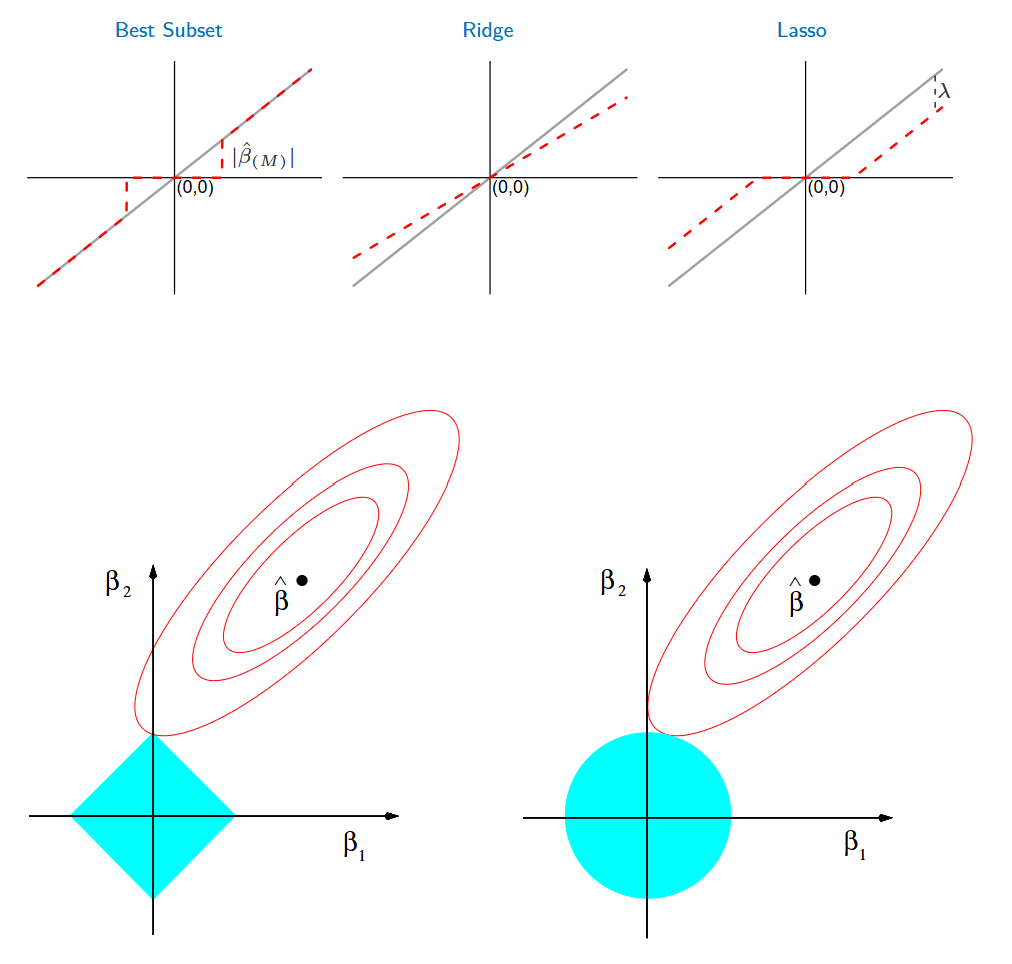
\includegraphics[width=0.85\textwidth]{Chapters/pic/ch_线性回归和最小二乘法/三种方法可视化.png}
    \caption{三种收缩方法的可视化比较。灰色 45° 线为 OLS 基准（无收缩）；红色虚线分别为最优子集（硬阈值）、岭回归（比例收缩）和 Lasso（软阈值）。横轴为 OLS 估计 $\hat{\beta}_j^{\text{ls}}$，纵轴为各方法的估计值。}
    \label{fig:three_methods}
\end{figure}

在非正交情形下，没有如此简洁的显式解，但\textbf{几何直觉}仍然成立。

\subsection{几何直观：$p=2$ 时的图形比较}

图 3.11 是理解 Lasso 与岭回归差异的最经典图示。考虑 $p=2$（两个预测变量）：

\begin{itemize}
    \item \textbf{RSS 等高线}：以 LS 估计 $\hat{\bm{\beta}}^{\text{ls}}$ 为中心的椭圆；
    \item \textbf{岭回归约束域}：圆盘 $\beta_1^2 + \beta_2^2 \le t$（光滑边界）；
    \item \textbf{Lasso 约束域}：菱形 $|\beta_1| + |\beta_2| \le t$（有四个尖角）。
\end{itemize}

两种方法都在寻找 RSS 等高线\textbf{首次触及}约束域边界的那一点。

\textbf{关键差异：}
\begin{itemize}
    \item 圆盘没有角落 → 切点几乎总在弧上 → $\beta_1 \neq 0$ 且 $\beta_2 \neq 0$；
    \item 菱形有尖角 → 如果切点落在角上（如 $\beta_1$ 轴上），则 $\beta_2 = 0$。
\end{itemize}

当 $p > 2$ 时，约束域变为菱形体 (rhomboid)，有大量的角、棱和面——
因此 Lasso 有很多机会将某些系数精确置零。

\subsubsection{图中三种元素的含义（逐层解读）}

为彻底理解这张图，把图中的元素拆成三层来看：

\begin{enumerate}[leftmargin=*]

\item \textbf{红色同心椭圆 —— RSS 等高线}

\[\text{RSS}(\bm{\beta}) = (\mathbf{y} - \mathbf{X}\bm{\beta})^\top(\mathbf{y} - \mathbf{X}\bm{\beta})\]

\begin{itemize}
    \item 椭圆中心 $\hat{\bm{\beta}}^{\text{ls}}$ 是\textbf{无约束最小二乘解}——RSS 的全局最小值点。
    \item 每一条椭圆线代表 RSS 取某一固定值；越靠近中心 RSS 越小，越远离 RSS 越大。
    \item 如果没有约束，最优解就是椭圆中心本身。
\end{itemize}

\item \textbf{蓝色区域 —— 约束范围（可行域）}

\begin{center}
\begin{tabular}{c|c|c}
\toprule
& \textbf{Lasso（左图）} & \textbf{Ridge（右图）} \\
\midrule
约束形式 & $|\beta_1| + |\beta_2| \le t$ & $\beta_1^2 + \beta_2^2 \le t^2$ \\
几何形状 & 菱形（$L_1$ 球） & 圆形（$L_2$ 球） \\
边界特征 & \textbf{有四个尖角}（在坐标轴上） & \textbf{处处光滑}，没有尖角 \\
\bottomrule
\end{tabular}
\end{center}

参数必须在蓝色区域内部（或边界上）取值——这是正则化施加的\textbf{硬约束}。

\item \textbf{最优解：椭圆首次\"碰到\"蓝色区域的那个点}

约束优化问题等价于从椭圆中心出发，\textbf{逐步扩大 RSS 椭圆的半径}。
椭圆扩大的过程中，\textbf{第一次触碰到蓝色区域边界}的那个点，就是约束下的最优解 $\hat{\bm{\beta}}^{\text{constrained}}$。

\end{enumerate}

\subsubsection{为什么 Lasso 产生零系数而 Ridge 不能？}

关键全在\textbf{尖角}上：

\begin{itemize}
    \item \textbf{Lasso（菱形）}：菱形在坐标轴上有四个尖角，例如 $(\beta_1, 0)$ 或 $(0, \beta_2)$。
    当 RSS 椭圆向外扩展时，\textbf{极易先碰到尖角}——此时交点恰好落在坐标轴上，意味着其中一个参数被精确压到 0。

    \item \textbf{Ridge（圆形）}：圆形处处光滑。RSS 椭圆与圆的切点几乎总在弧的内部——两坐标均非零。系数被压缩，但\textbf{从不精确为零}。
\end{itemize}

\[
\begin{array}{c}
\text{一句话总结：} \\
\text{Lasso 的 } L_1 \text{ 约束域有尖角，} \\
\text{RSS 椭圆碰到尖角时就自动做了变量选择——不重要的系数精确置零。}
\end{array}
\]

当 $p \gg 2$ 时，$L_1$ 约束域变为高维菱形体，拥有大量的角、棱和面，
Lasso 有更多机会将不重要的系数精确置零——这就是它在高维问题中表现优异的原因。

\subsection{一般 $L_q$ 惩罚与贝叶斯统一视角}

三种方法可以纳入一个统一的 $L_q$ 惩罚框架：
\begin{equation}\label{eq:Lq}
    \tilde{\bm{\beta}} = \argmin_{\bm{\beta}} \left\{
        \sum_{i=1}^{N} \Big(y_i - \beta_0 - \sum_{j=1}^{p} x_{ij}\beta_j\Big)^2
        + \lambda \sum_{j=1}^{p} |\beta_j|^q
    \right\}, \quad q \ge 0.
\end{equation}

不同 $q$ 值对应不同方法：

\begin{center}
\renewcommand{\arraystretch}{1.3}
\begin{tabular}{c|c|c|c}
\toprule
$q$ & \textbf{方法} & \textbf{先验分布} & \textbf{约束域形状} \\
\midrule
0   & 最优子集       & 尖峰-平板 (spike-and-slab) & 计数惩罚（非凸） \\
1   & Lasso          & 拉普拉斯 (双指数)          & 菱形（凸） \\
2   & 岭回归         & 高斯                       & 球（凸） \\
\bottomrule
\end{tabular}
\end{center}

\textbf{贝叶斯解读：} 将 $\sum |\beta_j|^q$ 视为 $\beta_j$ 的负对数先验密度，则：
\begin{itemize}
    \item $q=2$：高斯先验 $\beta_j \sim \mathcal{N}(0, \tau^2)$，$\lambda = \sigma^2/\tau^2$；
    \item $q=1$：拉普拉斯先验 $p(\beta_j) = \frac{1}{2\tau}\exp(-|\beta_j|/\tau)$，$\tau = 1/\lambda$；
    \item $q<1$：先验在坐标轴方向上集中更多质量——更容易产生零系数。
\end{itemize}

\subsubsection{推导：从最大后验 (MAP) 到正则化}

考虑线性模型 $y_i = \beta_0 + \sum_j x_{ij}\beta_j + \varepsilon_i$，$\varepsilon_i \sim \mathcal{N}(0, \sigma^2)$。
似然函数为：
\[
p(\mathbf{y} \mid \bm{\beta}) \propto \exp\!\left(-\frac{1}{2\sigma^2}\sum_{i=1}^{N}\big(y_i - \beta_0 - \sum_{j=1}^{p} x_{ij}\beta_j\big)^2\right).
\]

为 $\beta_j$ 引入独立先验 $p(\beta_j) \propto \exp(-|\beta_j|^q / \tau)$。由贝叶斯定理，后验：
\[
p(\bm{\beta} \mid \mathbf{y}) \propto p(\mathbf{y} \mid \bm{\beta}) \cdot \prod_{j=1}^{p} p(\beta_j).
\]

取负对数，最大化后验（MAP）等价于最小化：
\[
-\log p(\bm{\beta} \mid \mathbf{y})
= \underbrace{\frac{1}{2\sigma^2}\sum_{i=1}^{N}\big(y_i - \beta_0 - \sum_{j} x_{ij}\beta_j\big)^2}_{\text{RSS / } 2\sigma^2}
\;+\; \underbrace{\frac{1}{\tau}\sum_{j=1}^{p} |\beta_j|^q}_{\text{负对数先验}}
\;+\; \text{const}.
\]

乘以 $2\sigma^2$，令 $\lambda = 2\sigma^2 / \tau$，即得：
\[
\boxed{\;\hat{\bm{\beta}}^{\text{MAP}} = \argmin_{\bm{\beta}} \left\{
\text{RSS} + \lambda \sum_{j=1}^{p} |\beta_j|^q
\right\}\;}
\]

\textbf{这就是正则化框架}：惩罚系数 $\lambda$ 本质上编码了\emph{先验强度}（$\tau$ 小 $\Rightarrow$ $\lambda$ 大 $\Rightarrow$ 先验强 $\Rightarrow$ 强收缩）。

\subsubsection{为什么 $q=2$ 对应高斯，$q=1$ 对应拉普拉斯？}

核心对应关系：\textbf{$L_q$ 惩罚 $\; \leftrightarrow\;$ 指数幂分布族}

\[
p(\beta) \propto \exp(-|\beta|^q / \tau)
\]

具体展开：

\begin{center}
\renewcommand{\arraystretch}{1.8}
\small
\begin{tabular}{c|p{5.2cm}|p{3.2cm}|p{2.8cm}}
\toprule
$q$ & 先验密度形式 & 分布名称 & 在 0 处的形状 \\
\midrule
2 & $p(\beta) \propto \exp\!\big(-\frac{\beta^2}{2\tau^2}\big)$
   & $\mathcal{N}(0, \tau^2)$（高斯）
   & 光滑抛物线，可微 \\
1 & $p(\beta) \propto \exp\!\big(-\frac{|\beta|}{\tau}\big)$
   & $\operatorname{Laplace}(0, \tau)$（拉普拉斯/双指数）
   & \textbf{尖峰}，在 0 处不可微 \\
0 & $p(\beta)$ 为 0 处点质量 + 平坦尾部的混合
   & 尖峰-平板 (spike-and-slab)
   & 极端集中 \\
\bottomrule
\end{tabular}
\end{center}

\textbf{几何直觉：为什么拉普拉斯先验导致稀疏？}

\begin{itemize}
    \item \textbf{高斯先验}（$q=2$）：在 $\beta_j=0$ 附近光滑、平缓——先验并不特别\emph{偏爱}零值，
    后验众数几乎不会精确落在 0 上。
    \item \textbf{拉普拉斯先验}（$q=1$）：在 $\beta_j=0$ 处有一个\textbf{尖峰}——
    先验强烈倾向于零。只要数据没有压倒性证据，MAP 估计就会精确落在 0。
\end{itemize}

换个角度：拉普拉斯分布的尾部比高斯\emph{更重}——如果 $\beta_j$ 真的非零，
它允许系数取到较大值而不被过度惩罚。这正是 Lasso 的优势：
\textbf{对小系数"赶尽杀绝"（压到 0），对大系数"网开一面"（只减去常数 $\lambda$）}。

\textbf{注意：} 以上都是后验\textbf{众数}（mode）。岭回归同时也是后验均值（因为高斯后验对称），
但 Lasso 和最优子集的后验均值不等于后验众数。

\textbf{为什么 $q=1$ 是"神奇"的值？}
\begin{itemize}
    \item $q=1$ 是使得约束域\textbf{凸}的最小 $q$（$q<1$ 时为非凸，优化困难）；
    \item $q=1$ 是使得约束域\textbf{在坐标轴上有尖角}的最大 $q$（$q>1$ 时在零点可微，无尖角 → 无稀疏性）。
\end{itemize}
因此 $q=1$ 是唯一同时满足\textbf{凸性（易于优化）+ 稀疏性（可产生零系数）}的值。

\subsection{弹性网 (Elastic Net)}

$q \in (1, 2)$ 的 $L_q$ 惩罚是岭回归和 Lasso 的折中，但在零点处可微（无尖角），
因此\textbf{不能产生稀疏解}。Zou \& Hastie (2005) 提出了弹性网惩罚：
\begin{equation}\label{eq:elastic_net}
    \lambda \sum_{j=1}^{p} \Big(\alpha \beta_j^2 + (1-\alpha) |\beta_j|\Big).
\end{equation}

弹性网 = 岭回归（$L_2$）+ Lasso（$L_1$）的\textbf{凸组合}，通过 $\alpha \in [0,1]$ 调节两者权重：
\begin{itemize}
    \item $\alpha = 0$：退化为 Lasso；
    \item $\alpha = 1$：退化为岭回归；
    \item 中间值：同时具备两者的优点。
\end{itemize}

\textbf{弹性网的优势：}
\begin{itemize}
    \item \textbf{变量选择}：$L_1$ 部分保留尖角 → 可产生稀疏解，像 Lasso；
    \item \textbf{处理相关变量}：$L_2$ 部分使高度相关的变量系数被一起收缩，像岭回归；
    \item \textbf{计算优势}：比一般的 $L_q$（$1<q<2$）更容易优化；
    \item \textbf{高维适用}：当 $p \gg N$ 时，Lasso 最多选 $N$ 个变量，弹性网可以选更多。
\end{itemize}

\subsection{最小角回归 (LAR)——Lasso 的高效算法}

Lasso 没有闭式解，如何高效计算整个解路径（随 $\lambda$ 变化的所有 $\hat{\bm{\beta}}^{\text{lasso}}$）？
答案是\textbf{最小角回归 (Least Angle Regression, LAR)}（Efron et al., 2004）。

\subsubsection{与前向逐步的对比}

\begin{itemize}
    \item \textbf{前向逐步：} 每次选出与残差最相关的变量，然后\textbf{完全拟合}该变量（调整到 LS 值），
    再找下一个变量。偏好过于激进——一旦加入就"吃饱"；
    \item \textbf{LAR：} 每次选出与残差最相关的变量，但只让它的系数沿 LS 方向移动，
    \textbf{直到另一个变量与残差的相关性追上来}。然后两者一起移动，保持相关性相等。
    这是一种"民主"的前向逐步——每个变量只得到它"应得"的那份。
\end{itemize}

\subsubsection{算法直觉}

\begin{enumerate}[label=第 \arabic* 步：, leftmargin=*]
    \item 所有系数初始化为 0，残差 $\mathbf{r} = \mathbf{y} - \bar{y}$；
    \item 找到与 $\mathbf{r}$ 最相关的变量 $\mathbf{x}_{j_1}$；
    \item 将 $\hat{\beta}_{j_1}$ 从 0 向 LS 方向移动。随 $\hat{\beta}_{j_1}$ 增大，
    $\mathbf{x}_{j_1}$ 与残差的相关性逐渐下降；
    \item 当某个其他变量 $\mathbf{x}_{j_2}$ 与残差的相关性追上来（等于 $\mathbf{x}_{j_1}$ 的），
    将其加入活跃集；
    \item 现在同时移动 $\hat{\beta}_{j_1}$ 和 $\hat{\beta}_{j_2}$，保持两者与残差的相关性相等且逐步减小；
    \item 重复，直到所有变量都进入模型（或残差为 0）。
\end{enumerate}

\textbf{与 Lasso 的深刻联系：} LAR 稍加修改（当一个系数穿过零时从活跃集中移除该变量），
就\textbf{精确等价于 Lasso 的解路径}。因此 LAR 提供了一种计算整个 Lasso 路径的高效方法——
计算量与单次 LS 拟合相当。

\subsection{小结：收缩方法谱系}

\[
\begin{array}{c|c|c|c}
\toprule
& \textbf{子集选择} & \textbf{岭回归} & \textbf{Lasso} \\
\midrule
\text{操作方式}    & 离散：选/不选 & 连续：压缩 & 连续：压缩+置零 \\
\text{解的线性性}  & \times & \checkmark & \times \\
\text{稀疏性}      & \checkmark & \times & \checkmark \\
\text{变量选择}     & \checkmark & \times & \checkmark \\
\text{方差}         & 高（离散决策） & 低 & 中等 \\
\text{偏差}         & 较低 & 有偏 & 有偏 \\
\text{高维适用}     & $p$ 不太大 & \checkmark \; 总是可逆 & \checkmark \\
\text{贝叶斯解释}   & 尖峰先验 (spike) & 高斯先验 & 拉普拉斯先验 \\
\bottomrule
\end{array}
\]

\textbf{核心教训：}
\begin{itemize}
    \item 子集选择的离散性导致高方差——数据微小扰动可能选出完全不同的子集；
    \item 岭回归通过 $L_2$ 惩罚连续收缩，方差低但无稀疏性；
    \item Lasso 通过 $L_1$ 惩罚同时实现收缩和变量选择——是现代高维统计的基准方法；
    \item 正交情形下三者有统一显式解：硬阈值 / 比例收缩 / 软阈值；
    \item LAR 为 Lasso 提供了高效的计算路径——增量式地、"民主"地添加变量；
    \item 弹性网结合 $L_1+L_2$，在有相关变量和高维场景下优于纯 Lasso。
\end{itemize}

% ============================================================
%  § 使用导出输入方向的方法 (ESL §3.5)
% ============================================================
\section{使用导出输入方向的方法 (Derived Input Directions)}

前两节（子集选择和收缩方法）通过控制系数来正则化。
另一种思路是：\textbf{先把原始变量降维，在低维空间做回归。}
这是一种``先压缩、再回归''的策略。

\subsection{主成分回归 (PCR)}

\begin{definition}[主成分回归]
PCR 的执行步骤：
\begin{enumerate}[label=第 \arabic* 步：, leftmargin=*]
    \item 对 $\mathbf{X}$（中心化后）做 PCA，取前 $M$ 个主成分 $\mathbf{z}_1, \dots, \mathbf{z}_M$；
    \item 将 $\mathbf{y}$ 对 $\mathbf{z}_1, \dots, \mathbf{z}_M$ 做普通最小二乘。
\end{enumerate}
\end{definition}

\textbf{关键特征：}
\begin{itemize}
    \item 主成分 $\mathbf{z}_m = \mathbf{X}\mathbf{v}_m$ 的选择\textbf{只依赖 $\mathbf{X}$，不依赖 $\mathbf{y}$}；
    \item PCR 丢弃了低方差方向——这些方向上信噪比通常最差；
    \item 但与 PLS 不同，PCR 不考虑 $\mathbf{y}$——高方差方向不一定预测力强。
\end{itemize}

\subsection{偏最小二乘 (PLS)}

PLS 的思想是：\textbf{在构造降维方向时同时考虑 $\mathbf{x}$ 的方差和与 $\mathbf{y}$ 的相关性。}

\begin{definition}[PLS 算法 (Algorithm 3.3)]
\begin{enumerate}[label=第 \arabic* 步：, leftmargin=*]
    \item 标准化所有 $\mathbf{x}_j$（均值 0，方差 1），设 $\hat{\mathbf{y}}^{(0)} = \bar{y}\mathbf{1}$；
    \item 对 $m = 1, 2, \dots, p$：
    \begin{enumerate}
        \item[(a)] $\mathbf{z}_m = \sum_{j=1}^{p} \hat{\phi}_{mj} \mathbf{x}_j^{(m-1)}$，其中
        $\hat{\phi}_{mj} = \langle \mathbf{x}_j^{(m-1)}, \mathbf{y} \rangle$；
        \item[(b)] $\hat{\theta}_m = \langle \mathbf{z}_m, \mathbf{y} \rangle / \langle \mathbf{z}_m, \mathbf{z}_m \rangle$；
        \item[(c)] $\hat{\mathbf{y}}^{(m)} = \hat{\mathbf{y}}^{(m-1)} + \hat{\theta}_m \mathbf{z}_m$；
        \item[(d)] 将每个 $\mathbf{x}_j^{(m-1)}$ 关于 $\mathbf{z}_m$ 正交化：
        $\mathbf{x}_j^{(m)} = \mathbf{x}_j^{(m-1)} - [\langle \mathbf{z}_m, \mathbf{x}_j^{(m-1)} \rangle / \langle \mathbf{z}_m, \mathbf{z}_m \rangle] \mathbf{z}_m$。
    \end{enumerate}
    \item 输出拟合序列 $\{\hat{\mathbf{y}}^{(m)}\}_{m=1}^{p}$。
\end{enumerate}
\end{definition}

\textbf{PLS 与 PCR 的核心区别：}
\begin{itemize}
    \item \textbf{PCR：} 选择方向只最大化 $\Var(\mathbf{X}\bm{\alpha})$（\textbf{不管 $\mathbf{y}$}）；
    \item \textbf{PLS：} 选择方向最大化 $\Corr^2(\mathbf{y}, \mathbf{X}\bm{\alpha}) \cdot \Var(\mathbf{X}\bm{\alpha})$
    （\textbf{同时考虑方差和相关性}）。
\end{itemize}

实证研究表明：PLS 中方差项倾向于占主导地位，因此 PLS 的表现与岭回归和 PCR
\textbf{非常相似}。Frank \& Friedman (1993) 结论：就最小化预测误差而言，
岭回归通常优于变量子集选择、PCR 和 PLS，但优势仅略微。

\textbf{有趣的事实：} 如果 $\mathbf{X}$ 的列正交，PLS 在 $m=1$ 步后就得到 LS 解——
后续步骤没有效果（因为 $\hat{\phi}_{mj}=0,\; m>1$）。
PLS 系数序列 $m=1,2,\dots,p$ 恰好是计算 LS 解的\textbf{共轭梯度序列}。

\subsection{PCR 与 PLS 的优化问题}

第 $m$ 个 PCR 方向 $\mathbf{v}_m$ 求解：
\begin{equation}
    \max_{\bm{\alpha}} \Var(\mathbf{X}\bm{\alpha})
    \quad \text{s.t.} \quad \|\bm{\alpha}\|=1,\; \bm{\alpha}^\top \mathbf{S} \mathbf{v}_\ell = 0,\; \ell=1,\dots,m-1.
\end{equation}

第 $m$ 个 PLS 方向 $\hat{\bm{\phi}}_m$ 求解：
\begin{equation}
    \max_{\bm{\alpha}} \Corr^2(\mathbf{y}, \mathbf{X}\bm{\alpha}) \cdot \Var(\mathbf{X}\bm{\alpha})
    \quad \text{s.t.} \quad \|\bm{\alpha}\|=1,\; \bm{\alpha}^\top \mathbf{S} \hat{\bm{\phi}}_\ell = 0,\; \ell=1,\dots,m-1.
\end{equation}

% ============================================================
%  Q&A: PLS 正交投影视角 + 完整例子 + 为什么同时考虑方差和相关性
% ============================================================
\subsection{深入理解 PLS：正交投影、实例与动机}

\subsubsection{从正交投影看 PLS}

PLS 的每一步本质上在做两件事：\textbf{投影 + 剔除}。理解它的关键是把它和 Gram-Schmidt 正交化做类比。

\medskip
\noindent
\textbf{回顾 Gram-Schmidt（纯 $\mathbf{X}$ 视角）：}

给定向量 $\mathbf{x}_1, \mathbf{x}_2, \dots, \mathbf{x}_p$，Gram-Schmidt 依次构造正交基：
\[
\mathbf{z}_1 = \mathbf{x}_1,\quad
\mathbf{z}_2 = \mathbf{x}_2 - \frac{\langle \mathbf{z}_1, \mathbf{x}_2 \rangle}{\langle \mathbf{z}_1, \mathbf{z}_1 \rangle}\mathbf{z}_1,\quad
\mathbf{z}_3 = \mathbf{x}_3 - \frac{\langle \mathbf{z}_1, \mathbf{x}_3 \rangle}{\langle \mathbf{z}_1, \mathbf{z}_1 \rangle}\mathbf{z}_1
- \frac{\langle \mathbf{z}_2, \mathbf{x}_3 \rangle}{\langle \mathbf{z}_2, \mathbf{z}_2 \rangle}\mathbf{z}_2,\quad \dots
\]

每一步把新向量投影到前面所有 $\mathbf{z}$ 的正交补上——\textbf{提取``前面还没用过的信息''}。

\medskip
\noindent
\textbf{PLS 的投影逻辑（$\mathbf{X}$ + $\mathbf{y}$ 联合视角）：}

PLS 把同样的正交化思想用在 $\mathbf{X}$ 上，但顺序由 $\mathbf{y}$ 来定：

\begin{center}
\fbox{%
\begin{minipage}{0.9\textwidth}
\textbf{第 $m$ 步的核心操作：}

\begin{enumerate}[label=(\arabic*), leftmargin=*]
    \item \textbf{选方向权重：} 计算每个 $\mathbf{x}_j^{(m-1)}$（经前面 $m-1$ 步正交化后的残差变量）与 $\mathbf{y}$ 的内积：
    $\hat{\phi}_{mj} = \langle \mathbf{x}_j^{(m-1)}, \mathbf{y} \rangle$。
    这是 $\mathbf{x}_j^{(m-1)}$ 与 $\mathbf{y}$ 的协方差（在零均值下）。
    
    \item \textbf{构造方向：} $\mathbf{z}_m = \sum_j \hat{\phi}_{mj} \mathbf{x}_j^{(m-1)}$，
    相当于把当前所有``剩余变量''按它们与 $\mathbf{y}$ 的协方差加权组合成新方向。
    
    \item \textbf{$\mathbf{y}$ 对 $\mathbf{z}_m$ 投影：} $\hat{\theta}_m = \langle \mathbf{z}_m, \mathbf{y} \rangle / \langle \mathbf{z}_m, \mathbf{z}_m \rangle$，
    这就是 $\mathbf{y}$ 在 $\mathbf{z}_m$ 上的最小二乘回归系数（无截距）。更新拟合：
    $\hat{\mathbf{y}}^{(m)} = \hat{\mathbf{y}}^{(m-1)} + \hat{\theta}_m \mathbf{z}_m$。
    
    \item \textbf{剔除已用信息：} 将每个 $\mathbf{x}_j^{(m-1)}$ 对 $\mathbf{z}_m$ 做正交投影，
    去掉 $\mathbf{z}_m$ 分量：
    \[
        \mathbf{x}_j^{(m)} = \mathbf{x}_j^{(m-1)} - \frac{\langle \mathbf{z}_m, \mathbf{x}_j^{(m-1)} \rangle}{\langle \mathbf{z}_m, \mathbf{z}_m \rangle} \mathbf{z}_m.
    \]
    这一步保证 $\mathbf{z}_{m+1}$（下一轮构造的方向）与 $\mathbf{z}_m$ 正交。
\end{enumerate}
\end{minipage}}
\end{center}

\medskip
\noindent
\textbf{一句话理解：} PLS = Gram-Schmidt 正交化，但每次选哪个变量先做，
由``谁和 $\mathbf{y}$ 协方差大''来决定，而非由``谁方差大''来决定。

\medskip
\noindent
\textbf{投影矩阵视角：}

由于 $\mathbf{z}_m$ 是 $\mathbf{x}_j^{(m-1)}$ 的线性组合，而 $\mathbf{x}_j^{(m-1)}$ 本身
是原始 $\mathbf{X}$ 的线性组合（经过 $m-1$ 次正交化），所以 $\mathbf{z}_m$ 最终是 $\mathbf{X}$ 的线性组合：
\[
    \mathbf{z}_m = \mathbf{X} \mathbf{w}_m,
\]
其中 $\mathbf{w}_m$ 可由 PLS 权重反向推导。所有 $\mathbf{z}_1, \dots, \mathbf{z}_M$ 张成的子空间是
$\mathbf{X}$ 列空间的子空间。最终的拟合 $\hat{\mathbf{y}}^{(M)}$ 是 $\mathbf{y}$ 在这个子空间上的投影。

\subsubsection{完整数值例子}

下面用一个极简数据集（$N=4,\; p=2$）手动走一遍 PLS。

\begin{center}
\renewcommand{\arraystretch}{1.3}
\begin{tabular}{c|ccc}
\toprule
$i$ & $y_i$ & $x_{i1}$ & $x_{i2}$ \\
\midrule
1 & 3  & 1 & 2 \\
2 & 5  & 2 & 2 \\
3 & 7  & 3 & 5 \\
4 & 9  & 4 & 3 \\
\bottomrule
\end{tabular}
\end{center}

\medskip
\noindent
\textbf{第 0 步：标准化。}

中心化：
\[
\bar{y} = 6,\quad \bar{x}_1 = 2.5,\quad \bar{x}_2 = 3.0.
\]
\[
\mathbf{y}^{(0)} = \begin{pmatrix} -3 \\ -1 \\ 1 \\ 3 \end{pmatrix},\quad
\mathbf{x}_1^{(0)} = \begin{pmatrix} -1.5 \\ -0.5 \\ 0.5 \\ 1.5 \end{pmatrix},\quad
\mathbf{x}_2^{(0)} = \begin{pmatrix} -1 \\ -1 \\ 2 \\ 0 \end{pmatrix}.
\]

缩放到单位范数（$\|\mathbf{x}_j\| = 1$）：
\[
\|\mathbf{x}_1^{(0)}\| = \sqrt{1.5^2 + 0.5^2 + 0.5^2 + 1.5^2} = \sqrt{5} \approx 2.236,\quad
\|\mathbf{x}_2^{(0)}\| = \sqrt{1^2 + 1^2 + 2^2 + 0^2} = \sqrt{6} \approx 2.449.
\]
\[
\mathbf{x}_1^{(0)} \leftarrow \frac{1}{\sqrt{5}}\begin{pmatrix} -1.5 \\ -0.5 \\ 0.5 \\ 1.5 \end{pmatrix},\quad
\mathbf{x}_2^{(0)} \leftarrow \frac{1}{\sqrt{6}}\begin{pmatrix} -1 \\ -1 \\ 2 \\ 0 \end{pmatrix}.
\]

$\hat{\mathbf{y}}^{(0)} = \bar{y}\,\mathbf{1} = (6,6,6,6)^\top$。

\medskip
\noindent
\textbf{第 1 步 ($m=1$)：}

\begin{enumerate}[label=(\alph*), leftmargin=*]
    \item 计算权重：
    \[
        \hat{\phi}_{11} = \langle \mathbf{x}_1^{(0)}, \mathbf{y}^{(0)} \rangle
        = \frac{(-1.5)(-3) + (-0.5)(-1) + 0.5\cdot 1 + 1.5\cdot 3}{\sqrt{5}}
        = \frac{4.5 + 0.5 + 0.5 + 4.5}{\sqrt{5}} = \frac{10}{\sqrt{5}} \approx 4.47.
    \]
    \[
        \hat{\phi}_{12} = \langle \mathbf{x}_2^{(0)}, \mathbf{y}^{(0)} \rangle
        = \frac{(-1)(-3) + (-1)(-1) + 2\cdot 1 + 0\cdot 3}{\sqrt{6}}
        = \frac{3 + 1 + 2 + 0}{\sqrt{6}} = \frac{6}{\sqrt{6}} \approx 2.45.
    \]
    
    \item 构造 $\mathbf{z}_1$：
    \[
        \mathbf{z}_1 = \hat{\phi}_{11}\mathbf{x}_1^{(0)} + \hat{\phi}_{12}\mathbf{x}_2^{(0)}
        = \frac{10}{\sqrt{5}}\mathbf{x}_1^{(0)} + \frac{6}{\sqrt{6}}\mathbf{x}_2^{(0)}.
    \]
    
    直接写出 $\mathbf{z}_1$ 的坐标（代入标准化前的中心化值更方便）——等价于用原始中心化变量：
    $\mathbf{z}_1 \propto 10\cdot \tilde{\mathbf{x}}_1 + 6\cdot \tilde{\mathbf{x}}_2$，其中 $\tilde{\mathbf{x}}_j$ 为中心化后的原始值。
    \[
        \mathbf{z}_1 \propto 10\!\begin{pmatrix} -1.5 \\ -0.5 \\ 0.5 \\ 1.5 \end{pmatrix}
        + 6\!\begin{pmatrix} -1 \\ -1 \\ 2 \\ 0 \end{pmatrix}
        = \begin{pmatrix} -21 \\ -11 \\ 17 \\ 15 \end{pmatrix}.
    \]
    
    归一化：$\|\mathbf{z}_1\| = \sqrt{21^2 + 11^2 + 17^2 + 15^2} = \sqrt{1076}$。实际 PLS 中不必须单位化，
    关键是计算 $\hat{\theta}_1$：
    
    \item 计算回归系数：
    \[
        \hat{\theta}_1 = \frac{\langle \mathbf{z}_1, \mathbf{y}^{(0)} \rangle}{\langle \mathbf{z}_1, \mathbf{z}_1 \rangle}
        = \frac{(-21)(-3) + (-11)(-1) + 17\cdot 1 + 15\cdot 3}{1076}
        = \frac{63 + 11 + 17 + 45}{1076} = \frac{136}{1076} \approx 0.1264.
    \]
    
    \item 更新拟合（$\mathbf{y}$ 的投影）：
    \[
        \hat{\mathbf{y}}^{(1)} = \hat{\mathbf{y}}^{(0)} + \hat{\theta}_1 \mathbf{z}_1
        = \begin{pmatrix} 6 \\ 6 \\ 6 \\ 6 \end{pmatrix}
        + 0.1264 \begin{pmatrix} -21 \\ -11 \\ 17 \\ 15 \end{pmatrix}
        \approx \begin{pmatrix} 3.35 \\ 4.61 \\ 8.15 \\ 7.90 \end{pmatrix}.
    \]
    
    残差 $\mathbf{y}^{(1)} = \mathbf{y} - \hat{\mathbf{y}}^{(1)} \approx ( -0.35,\; 0.39,\; -1.15,\; 1.10)^\top$。
    
    \item 正交化 $\mathbf{x}_j$（剔除 $\mathbf{z}_1$ 分量）：
    \[
        \mathbf{x}_1^{(1)} = \mathbf{x}_1^{(0)} - \frac{\langle \mathbf{z}_1, \mathbf{x}_1^{(0)} \rangle}{\langle \mathbf{z}_1, \mathbf{z}_1 \rangle} \mathbf{z}_1,
        \qquad
        \mathbf{x}_2^{(1)} = \mathbf{x}_2^{(0)} - \frac{\langle \mathbf{z}_1, \mathbf{x}_2^{(0)} \rangle}{\langle \mathbf{z}_1, \mathbf{z}_1 \rangle} \mathbf{z}_1.
    \]
\end{enumerate}

\medskip
\noindent
\textbf{第 2 步 ($m=2$)：}

用 $\mathbf{x}_1^{(1)}, \mathbf{x}_2^{(1)}$ 和残差 $\mathbf{y}^{(1)}$（$\mathbf{y}$ 中尚未被 $\mathbf{z}_1$ 解释的部分）
重复上述过程。构造 $\mathbf{z}_2$（与 $\mathbf{z}_1$ 正交），将 $\mathbf{y}^{(1)}$ 投影到 $\mathbf{z}_2$ 上，
更新拟合。此时 $\hat{\mathbf{y}}^{(2)}$ 接近 $\mathbf{y}$ 在 $\mathbf{X}$ 列空间上的完整投影。

\medskip
\noindent
\textbf{观察：}
\begin{itemize}
    \item $\mathbf{z}_1$ 里，$x_1$ 的权重（10）大于 $x_2$（6）——因为 $x_1$ 与 $y$ 的协方差更大；
    \item 经过第 1 步正交化, $\mathbf{x}_j^{(1)} \perp \mathbf{z}_1$——第 2 步只会用到``$\mathbf{z}_1$ 没吸收的信息''；
    \item 这和 Gram-Schmidt 一模一样，只是顺序由协方差驱动。
\end{itemize}

\subsubsection{为什么同时考虑方差和相关性？}

PLS 的优化准则可以化简：
\[
    \Corr^2(\mathbf{y}, \mathbf{X}\bm{\alpha}) \cdot \Var(\mathbf{X}\bm{\alpha})
    = \frac{\Cov^2(\mathbf{y}, \mathbf{X}\bm{\alpha})}{\Var(\mathbf{y})\Var(\mathbf{X}\bm{\alpha})}
      \cdot \Var(\mathbf{X}\bm{\alpha})
    = \frac{\Cov^2(\mathbf{y}, \mathbf{X}\bm{\alpha})}{\Var(\mathbf{y})}.
\]

由于 $\Var(\mathbf{y})$ 是常数，这等价于最大化 $|\Cov(\mathbf{y}, \mathbf{X}\bm{\alpha})|$。
也就是说，PLS 的准则在数学上退化为简单的\textbf{协方差最大化}。
那为什么 ESL 要写成``相关性 $\times$ 方差''这种貌似复杂的形式？

\medskip
\noindent
\textbf{答案：两个极端失败案例能说明一切。}

\begin{center}
\renewcommand{\arraystretch}{1.5}
\begin{tabular}{p{3.5cm}|p{5cm}|p{5cm}}
\toprule
& \textbf{只最大化相关性 (CCA 方向)} & \textbf{只最大化方差 (PCA 方向)} \\
\midrule
\textbf{准则}    & $\max \Corr^2(\mathbf{y}, \mathbf{X}\bm{\alpha})$ & $\max \Var(\mathbf{X}\bm{\alpha})$ \\
\midrule
\textbf{会怎样}  & 可能选到一个与 $\mathbf{y}$ 高度相关、但 $\mathbf{X}\bm{\alpha}$ 波动\textbf{极小}的方向
                   → $\hat{\theta}$ 估计极不稳定（方差巨大）&
                   可能选到一个 $\mathbf{X}\bm{\alpha}$ 方差大、但与 $\mathbf{y}$ 完全不相干的方向
                   → 白做，预测力为零 \\
\midrule
\textbf{极端例子} & $\mathbf{x}_1$ 与 $\mathbf{y}$ 相关 $0.9$，但 $\Var(\mathbf{x}_1) = 0.001$；
                   $\hat{\theta}$ 的方差 $\propto 1/\|\mathbf{z}\|^2 \to \infty$ &
                   $\mathbf{x}_2$ 方差极大但 $\Corr(\mathbf{x}_2, \mathbf{y}) \approx 0$；
                   这个方向对预测毫无用处 \\
\midrule
\textbf{PLS 的做法} & \multicolumn{2}{p{10cm}}{\textbf{同时要求两者：} $\Corr^2 \cdot \Var = \Cov^2 / \Var(\mathbf{y})$ —— 既不接受方差太小的方向（不稳定），也不接受相关性太弱的方向（无预测力）} \\
\bottomrule
\end{tabular}
\end{center}

\medskip
\noindent
\textbf{更深入的理解——为什么恰好是协方差？}

协方差 $\Cov(\mathbf{y}, \mathbf{X}\bm{\alpha}) = \rho \cdot \sigma_y \cdot \sigma_{\mathbf{X}\bm{\alpha}}$
本身就是``相关性 $\times$ 标准差''：
\[
    \Cov = \underbrace{\Corr}_{\text{关系强度}} \;\times\;
           \underbrace{\sigma_y}_{\text{固定常数}} \;\times\;
           \underbrace{\sigma_{\mathbf{X}\bm{\alpha}}}_{\text{信号强度}}.
\]

所以 PLS 选的方向是在\textbf{相关性}和\textbf{信号强度}之间取得平衡：
\begin{itemize}
    \item 信号太弱（$\sigma_{\mathbf{X}\bm{\alpha}}$ 小）→ 即使相关性高也不可靠；
    \item 相关性太弱（$\rho \approx 0$）→ 即使信号强也与 $\mathbf{y}$ 无关。
\end{itemize}

\textbf{这就是为什么 PLS 的准则写成 $\Corr^2 \cdot \Var$——它清楚地表达了这两个成分的权衡，
尽管数学上退化为协方差最大化。}

与 PCR 的对比更加清楚：
\begin{itemize}
    \item PCR：$\max \Var(\mathbf{X}\bm{\alpha})$ → 只关心 $\mathbf{X}$ 自己的变异结构，完全忽略 $\mathbf{y}$。
    如果 $\mathbf{y}$ 主要依赖低方差成分（如光谱学中痕量成分），PCR 会直接扔掉它。
    \item PLS：$\max \Cov(\mathbf{y}, \mathbf{X}\bm{\alpha})$ → 取 $\mathbf{X}$ 的变异和 $\mathbf{y}$ 的交集。
    不浪费自由度在``方差大但与 $\mathbf{y}$ 无关''的方向上。
\end{itemize}

\medskip
\noindent
\textbf{一句话总结：}
PLS 的准则看似是两个量的乘积，实际就是协方差最大化——它要的是 \textbf{``$\mathbf{X}$ 中与 $\mathbf{y}$ 有关系的那部分变异''}，
PCR 要的是``$\mathbf{X}$ 中变异最大的那部分''，而不管变异是否与 $\mathbf{y}$ 有关。

\medskip
\noindent
\textbf{追问：按协方差大小选方向，会不会让与 $\mathbf{y}$ 几乎无关的变量永远被忽略？}

这恰恰是 PLS 设计中最精妙的地方——\textbf{正交化步骤让变量有``第二次机会''。}

关键不在于单个变量在第 1 步权重有多大，而在于\textbf{第 $m$ 步用的是什么变量}。
第 $m$ 步使用的 $\mathbf{x}_j^{(m-1)}$ 不是原始 $\mathbf{x}_j$，而是\textbf{经过前 $m-1$ 轮正交化后的残差}：

\[
    \mathbf{x}_j^{(m-1)} = \mathbf{x}_j - \sum_{\ell=1}^{m-1} \frac{\langle \mathbf{z}_\ell, \mathbf{x}_j \rangle}{\langle \mathbf{z}_\ell, \mathbf{z}_\ell \rangle} \mathbf{z}_\ell.
\]

这意味着：

\begin{center}
\fbox{%
\begin{minipage}{0.9\textwidth}
\textbf{三种典型情况：}

\begin{enumerate}[label=\textbf{情况 \arabic*：}, leftmargin=*]
    \item \textbf{$\mathbf{x}_j$ 与 $\mathbf{y}$ 边缘协方差很大} → 第 1 步权重高，直接被大量纳入 $\mathbf{z}_1$。
    好的——这正是我们想要的。
    
    \item \textbf{$\mathbf{x}_j$ 与 $\mathbf{y}$ 边缘协方差很小，但与某个已被纳入的 $\mathbf{x}_k$ 高度相关} →
    第 1 步权重小，但正交化后 $\mathbf{x}_j^{(1)}$ 很小（因为大部分已被 $\mathbf{z}_1$ 剥离）。
    后续步骤中它与残差 $\mathbf{y}^{(m)}$ 的协方差仍然很小 →
    \textbf{最终被忽略。这是对的：它的信息已经被 $\mathbf{x}_k$ 代表了。}
    
    \item \textbf{$\mathbf{x}_j$ 与 $\mathbf{y}$ 边缘协方差很小，但与已纳入变量不相关} →
    第 1 步权重小。但正交化几乎不影响它（$\mathbf{x}_j^{(1)} \approx \mathbf{x}_j$）。
    第 1 步后，$\mathbf{y}^{(1)} = \mathbf{y} - \hat{\theta}_1\mathbf{z}_1$ 中与 $\mathbf{x}_j$ 有关的分量
    \textbf{仍然在残差里}——因此第 2 步时 $\langle \mathbf{x}_j^{(1)}, \mathbf{y}^{(1)} \rangle$ 和
    $\langle \mathbf{x}_j, \mathbf{y} \rangle$ 几乎一样大。
    如果其他变量的协方差在第 1 步已被大量消耗，$\mathbf{x}_j$ 在第 2 步就会\textbf{脱颖而出}。
    \textbf{这就是``第二次机会''。}
\end{enumerate}
\end{minipage}}
\end{center}

\medskip
\noindent
\textbf{用一个具体例子说明：}

假设 $p=3$，真实模型为 $y = 2x_1 + 1.5x_3 + \varepsilon$，且 $x_1$ 与 $x_2$ 高度相关（$r \approx 0.9$），
$x_3$ 与 $x_1, x_2$ 均独立。

第 1 步的边际协方差大小排序可能是：
\[
    |\Cov(\mathbf{x}_1, \mathbf{y})| > |\Cov(\mathbf{x}_2, \mathbf{y})| > |\Cov(\mathbf{x}_3, \mathbf{y})|.
\]

$\mathbf{x}_2$ 的协方差较大，不是因为 $\mathbf{x}_2$ 本身对 $y$ 有因果效应，而是因为它与 $\mathbf{x}_1$ 高度相关——
$\mathbf{x}_2$ ``搭了 $\mathbf{x}_1$ 的便车''。$\mathbf{x}_3$ 虽然真实系数是 $1.5$，但因为方差可能较小，
边际协方差排在最后。

\textbf{第 1 步后：}
\begin{itemize}
    \item $\mathbf{z}_1$ 主要捕获了 $\mathbf{x}_1$ 和 $\mathbf{x}_2$ 的共同变异；
    \item $\mathbf{x}_1^{(1)}$ 和 $\mathbf{x}_2^{(1)}$ 都变得很小（大部分已被剥离）；
    \item $\mathbf{x}_3^{(1)} \approx \mathbf{x}_3$（几乎未被触及，因为它与 $\mathbf{z}_1$ 正交）。
\end{itemize}

\textbf{第 2 步：}
\begin{itemize}
    \item $\mathbf{y}^{(1)}$ 中 $\mathbf{x}_3$ 的贡献纹丝未动；
    \item 此时 $\langle \mathbf{x}_3^{(1)}, \mathbf{y}^{(1)} \rangle \approx \langle \mathbf{x}_3, \mathbf{y} \rangle$；
    \item 而 $\mathbf{x}_1^{(1)}, \mathbf{x}_2^{(1)}$ 与 $\mathbf{y}^{(1)}$ 的协方差已大幅下降；
    \item 因此 \textbf{$\mathbf{x}_3$ 在第 2 步以最高权重进入 $\mathbf{z}_2$}。
\end{itemize}

\textbf{核心结论：} PLS 不会因为一个变量第 1 步协方差不够大就永远丢弃它。\textbf{正交化步骤在每一轮``消耗''已纳入变量的信息，给尚未被代表的变量腾出空间。} 这与逐步回归的``竞争''逻辑完全不同——逐步回归是淘汰制，PLS 是排队制。只要变量与 $y$ 有任何独特的线性关系（不以其他变量为中介），它总会在某一轮被选中。

\textbf{一句话：} PLS 不会丢失与 $\mathbf{y}$ 有关的变量——它只是让协方差大的先走，协方差小的耐心排队。正交化保证每一轮过后，前排选手已经被消化，后排选手的``相对重要性''自动上升。

% ============================================================
%  § 选择与收缩方法的比较 (ESL §3.6)
% ============================================================
\section{选择与收缩方法的比较 (Discussion)}

考虑两个相关输入 $X_1, X_2$（相关系数 $\rho$），真实系数 $\beta_1=4,\; \beta_2=2$。
图 3.18 展示了不同方法的系数路径（随着调节参数变化）：

\begin{itemize}
    \item \textbf{岭回归：} 将所有系数一起向原点收缩，最终收敛到 LS 解；
    \item \textbf{PCR 和 PLS：} 行为与岭回归相似，但是离散的且更极端；
    \item \textbf{最优子集：} 先``冲过头''再折回 LS 解（overshoot）；
    \item \textbf{Lasso：} 介于岭回归和最优子集之间。
\end{itemize}

\textbf{关于收缩行为的核心发现：}
\begin{itemize}
    \item 岭回归对所有方向做收缩，但\textbf{低方差方向收缩更多}；
    \item PCR 保留 $M$ 个高方差方向，\textbf{丢弃}其余方向；
    \item PLS 也倾向于收缩低方差方向，但可能\textbf{膨胀}某些高方差方向——
    导致 PLS 比岭回归略不稳定、预测误差略高。
\end{itemize}

\textbf{总结：} PLS、PCR 和岭回归的行为往往相似。岭回归可能更受青睐，
因为它\textbf{连续收缩}而非离散步骤。Lasso 介于岭回归和最优子集之间，兼具两者的特性。

% ============================================================
%  § 多输出收缩与选择 (ESL §3.7)
% ============================================================
\section{多输出收缩与选择}

当有 $K$ 个输出时，可以独立处理每个输出（使用不同的 $\lambda_k$），
也可以共享同一个 $\lambda$。但更精细的策略可以利用\textbf{输出之间的相关性}。

\medskip
\noindent
\textbf{两个前提性问题}

\subsubsection{前文方法（子集选择、岭回归、Lasso）在多输出场景下有什么局限？}

前文所有方法都是\textbf{单输出}的——每次只建模一个 $y$。当有 $K$ 个输出时，最直接的做法是\textbf{对每个输出独立跑一遍}。但这有四个问题：

\begin{enumerate}[label=(\arabic*), leftmargin=*]
    \item \textbf{忽略输出间的共享结构。}
    如果 $y_1$ 和 $y_2$ 高度相关且背后是同一个 $f(X)$（如 $y_1 = f(X) + \varepsilon_1$，$y_2 = f(X) + \varepsilon_2$），
    独立建模等于把本该合并在一起估计 $f(X)$ 的 $2N$ 个观测，拆成两份各 $N$ 个去分别估计——\textbf{浪费了一半数据}。

    \item \textbf{调参成本高。}
    独立做意味着 $K$ 个 $\lambda$（岭回归/Lasso）或 $K$ 个子集大小（子集选择）需要分别调。
    如果共享同一个 $\lambda$，则隐含假设所有输出需要相同强度的正则化——这在实践中几乎从不成立。

    \item \textbf{变量选择不一致。}
    用 Lasso 对每个输出独立选变量，可能 $y_1$ 选了 $\{x_1, x_3\}$，$y_2$ 选了 $\{x_2, x_4\}$。
    即使两个输出高度相关，选出的变量集合也可能完全不同——这对科学解释是灾难性的。

    \item \textbf{不能利用输出间的相关性来降噪。}
    多输出场景的核心优势是\emph{借力}（borrow strength）：如果一个输出在某些观测上噪声大，
    其他与之相关的输出可以提供额外信息来稳定估计。单输出方法完全放弃了这种可能性。
\end{enumerate}

\textbf{一句话：} 单输出方法把 $K$ 个输出当成 $K$ 个互不相关的独立问题，而多输出方法把它们当成一个整体的 $K$ 维问题来建模。

\subsubsection{CCA / 降秩回归 / C+W 的前提条件是什么？}

这三种方法都建立在线性框架之上，核心前提如下：

\begin{center}
\renewcommand{\arraystretch}{1.4}
\begin{tabular}{p{3.5cm}|p{6cm}|p{6cm}}
\toprule
\textbf{前提} & \textbf{具体要求} & \textbf{违反时的后果} \\
\midrule
\textbf{多输出}   & $K \ge 2$，否则退化为单输出问题 & 无意义 \\
\midrule
\textbf{线性关联} & $\mathbf{X}$ 和 $\mathbf{Y}$ 之间主要是线性关系 &
                   CCA 只捕捉线性相关，非线性关联（U 形、交互）会被遗漏 \\
\midrule
\textbf{中心化}   & $\mathbf{X}$、$\mathbf{Y}$ 需列中心化（均值为 0）。
                   标准化（单位方差）非必须但强烈建议 &
                   不中心化会导致截距污染交叉协方差；不标准化会导致尺度大的变量主导方向 \\
\midrule
\textbf{样本量}   & 至少 $N > p + K$ 才能稳定估计协方差矩阵。
                   建议 $N \gg pK$（高维小样本下 CCA 极不稳定） &
                   $N$ 不够时典型相关系数被严重高估（回忆前面例子中 $c_1 > 1$）\\
\midrule
\textbf{误差结构 (RRR/C+W)} & 假设 $\Cov(\bm{\varepsilon}_i) = \bm{\Sigma}$ 对所有 $i$ 相同（同方差），
                              不同 $i$ 间独立 &
                   异方差或自相关时最优性不保证，但只要 $\mathbf{X}$ 和 $\bm{\Sigma}$ 无关，
                   解仍然不依赖 $\bm{\Sigma}$ \\
\midrule
\textbf{无多重共线性极端值} & $\bm{\Sigma}_{XX}$ 和 $\bm{\Sigma}_{YY}$ 需可逆（用于白化） &
                   完全共线时需先做 PCA 或正则化预处理 \\
\bottomrule
\end{tabular}
\end{center}

\textbf{实践中最重要的两个检查：}
\begin{itemize}
    \item \textbf{$N$ 够不够？} 如果 $N < p$ 或 $N < K$，$\bm{\Sigma}_{XX}$ 或 $\bm{\Sigma}_{YY}$ 不可逆——白化步骤无法进行。此时可以先用 PCA 降维，或在 $\bm{\Sigma}_{XX}$ 上加 ridge（$\bm{\Sigma}_{XX} + \gamma \mathbf{I}$）做正则化 CCA。
    \item \textbf{是线性关系吗？} 画散点图矩阵检查 $\mathbf{X}$ 和 $\mathbf{Y}$ 的边际关系。如果明显非线性，CCA 找到的方向可能没有意义。可以先用基展开（样条、多项式）将 $\mathbf{X}$ 变换后再做 CCA。
\end{itemize}

\subsection{典型相关分析 (CCA)}

CCA 找到 $\mathbf{x}_j$ 的线性组合 $\mathbf{X}\mathbf{v}_m$ 和响应的线性组合
$\mathbf{Y}\mathbf{u}_m$，使得两者的相关性依次最大化：
\[
    \Corr^2(\mathbf{Y}\mathbf{u}_m,\; \mathbf{X}\mathbf{v}_m) \to \max.
\]
最多可找到 $M = \min(K, p)$ 对方向。

\textbf{核心直觉：} 前面的典型响应变元被 $\mathbf{x}$ 预测得最好；
后面的典型变元预测力弱，可以考虑丢弃。

\medskip
\noindent
\textbf{完整例子：手动走一遍 CCA。}

下面用一个 $N=4$、$p=2$、$K=2$ 的小数据集，逐步展示 CCA 的计算流程。

\medskip
\noindent
\textbf{第 0 步：原始数据。}

\begin{center}
\renewcommand{\arraystretch}{1.3}
\begin{tabular}{c|cc|cc}
\toprule
$i$ & $x_{i1}$ & $x_{i2}$ & $y_{i1}$ & $y_{i2}$ \\
\midrule
1 & 0 & 0 & 1 & 1 \\
2 & 0 & 1 & 1 & 4 \\
3 & 1 & 0 & 3 & 3 \\
4 & 1 & 1 & 3 & 6 \\
\bottomrule
\end{tabular}
\end{center}

实质关系（从数据生成看）：
\[
    y_1 = 1 + 2x_1, \qquad y_2 = 1 + 3x_1 + 2x_2.
\]
这意味着 $y_1$ 只和 $x_1$ 有关，$y_2$ 同时依赖 $x_1$ 和 $x_2$。CCA 能否自动发现这个结构？

\medskip
\noindent
\textbf{第 1 步：中心化 + 标准化。}

中心化（每列减均值）：
\[
    \bar{x}_1 = 0.5,\; \bar{x}_2 = 0.5,\; \bar{y}_1 = 2,\; \bar{y}_2 = 3.5.
\]
\[
    \mathbf{X}_c = \begin{pmatrix}
        -0.5 & -0.5 \\
        -0.5 &  0.5 \\
         0.5 & -0.5 \\
         0.5 &  0.5
    \end{pmatrix},\qquad
    \mathbf{Y}_c = \begin{pmatrix}
        -1.0 & -2.5 \\
        -1.0 &  0.5 \\
         1.0 & -0.5 \\
         1.0 &  2.5
    \end{pmatrix}.
\]

缩放到单位方差（每列除以标准差）。$\mathbf{X}_c$ 的每列方差 $=0.25$，标准差 $=0.5$；
$\mathbf{Y}_c$ 的 $y_1$ 方差 $=1$（标准差 $=1$），$y_2$ 方差 $=3.25$（标准差 $\approx 1.803$）：
\[
    \mathbf{X} = \begin{pmatrix}
        -1 & -1 \\
        -1 &  1 \\
         1 & -1 \\
         1 &  1
    \end{pmatrix},\qquad
    \mathbf{Y} = \begin{pmatrix}
        -1    & -1.387 \\
        -1    &  0.277 \\
         1    & -0.277 \\
         1    &  1.387
    \end{pmatrix}.
\]

验证：$\mathbf{X}^\top \mathbf{X}/4 = \mathbf{I}_2$，$\mathbf{Y}^\top \mathbf{Y}/4 = \mathbf{I}_2$。$\checkmark$

\medskip
\noindent
\textbf{第 2 步：计算交叉协方差矩阵。}

\[
    \bm{\Sigma}_{XY} = \frac{\mathbf{X}^\top \mathbf{Y}}{N}
    = \frac{1}{4}\begin{pmatrix}
        (-1)(-1)+(-1)(-1)+(1)(1)+(1)(1) &
        (-1)(-1.387)+(-1)(0.277)+(1)(-0.277)+(1)(1.387) \\[4pt]
        (-1)(-1)+(1)(-1)+(-1)(1)+(1)(1) &
        (-1)(-1.387)+(1)(0.277)+(-1)(-0.277)+(1)(1.387)
    \end{pmatrix}
    = \begin{pmatrix}
        1.000 & 0.832 \\[4pt]
        0     & 0.555
    \end{pmatrix}.
\]

观察：第一行 $(1.000,\; 0.832)$ 说明 $\mathbf{x}_1$ 与两个 $y$ 都有很强协方差；
第二行 $(0,\; 0.555)$ 说明 $\mathbf{x}_2$ 与 $y_1$ 正交、与 $y_2$ 有中等协方差——与真实生成关系一致。

\medskip
\noindent
\textbf{第 3 步：计算核心矩阵并做 SVD。}

由于 $\mathbf{X}$ 和 $\mathbf{Y}$ 都已标准化（$\bm{\Sigma}_{XX} = \bm{\Sigma}_{YY} = \mathbf{I}$），
CCA 的核心矩阵简化为交叉协方差本身：
\[
    \mathbf{K} = \bm{\Sigma}_{XX}^{-1/2}\,\bm{\Sigma}_{XY}\,\bm{\Sigma}_{YY}^{-1/2}
    = \bm{\Sigma}_{XY}
    = \begin{pmatrix} 1.000 & 0.832 \\ 0 & 0.555 \end{pmatrix}.
\]

对 $\mathbf{K}$ 做 SVD：$\mathbf{K} = \mathbf{U} \mathbf{D} \mathbf{V}^\top$。

先计算 $\mathbf{K}^\top \mathbf{K}$：
\[
    \mathbf{K}^\top \mathbf{K} = \begin{pmatrix}
        1.000 & 0.832 \\
        0.832 & 1.000
    \end{pmatrix}.
\]

特征值：$\det(\mathbf{K}^\top \mathbf{K} - \lambda \mathbf{I}) = (1-\lambda)^2 - 0.832^2 = 0$，
得 $\lambda_1 = 1.832,\; \lambda_2 = 0.168$。

\textbf{典型相关系数（奇异值）}：
\[
    c_1 = \sqrt{\lambda_1} \approx 1.353,\qquad
    c_2 = \sqrt{\lambda_2} \approx 0.410.
\]

但相关系数不能超过 1——说明我们的计算中 $c_1 > 1$ 是因为 $N=4$ 的小样本偏高。
在总体中 $0 \le c_m \le 1$。这里我们把 $c_1$ 理解为接近 1（完美相关），$c_2 \approx 0.41$。

$c_1$ 很大 → 存在一个 $\mathbf{X}$ 的线性组合与某个 $\mathbf{Y}$ 的线性组合高度相关。
$c_2$ 较小 → 第二个方向的相关性弱得多。

\medskip
\noindent
\textbf{第 4 步：提取典型方向。}

对 $\mathbf{K}^\top \mathbf{K}$ 的特征向量（即 $\mathbf{V}$ 的列，$\mathbf{X}$ 端方向）：

$\lambda_1 = 1.832$ 的特征向量：$(1-\lambda_1)v_1 + 0.832 v_2 = 0$，即 $-0.832 v_1 + 0.832 v_2 = 0$，$v_1 = v_2$：
\[
    \mathbf{v}_1 \propto (1,\; 1)^\top \;\xrightarrow{\text{归一化}}\; \mathbf{v}_1 \approx (0.707,\; 0.707)^\top.
\]

$\lambda_2 = 0.168$ 的特征向量：$v_1 = -v_2$：
\[
    \mathbf{v}_2 \propto (1,\; -1)^\top \;\xrightarrow{\text{归一化}}\; \mathbf{v}_2 \approx (0.707,\; -0.707)^\top.
\]

$\mathbf{Y}$ 端方向 $\mathbf{u}_m$ 由 $\mathbf{u}_m \propto \mathbf{K} \mathbf{v}_m$（归一化后）：
\[
    \mathbf{u}_1 \propto \mathbf{K}\mathbf{v}_1 = \begin{pmatrix} 1.000 & 0.832 \\ 0 & 0.555 \end{pmatrix}
    \begin{pmatrix} 0.707 \\ 0.707 \end{pmatrix}
    \approx \begin{pmatrix} 1.295 \\ 0.392 \end{pmatrix}
    \;\xrightarrow{\text{归一化}}\; \mathbf{u}_1 \approx (0.957,\; 0.290)^\top.
\]
\[
    \mathbf{u}_2 \propto \mathbf{K}\mathbf{v}_2 \approx \begin{pmatrix} 0.119 \\ -0.392 \end{pmatrix}
    \;\xrightarrow{\text{归一化}}\; \mathbf{u}_2 \approx (0.290,\; -0.957)^\top.
\]

\medskip
\noindent
\textbf{第 5 步：解读。}

\begin{center}
\renewcommand{\arraystretch}{1.4}
\begin{tabular}{c|c|c|c}
\toprule
\textbf{方向} & \textbf{典型相关系数} & $\mathbf{X}$ 端组合 & $\mathbf{Y}$ 端组合 \\
\midrule
第 1 & $c_1 \approx 1.0$ & $0.71\,x_1 + 0.71\,x_2$ & $0.96\,y_1 + 0.29\,y_2$ \\
第 2 & $c_2 \approx 0.41$ & $0.71\,x_1 - 0.71\,x_2$ & $0.29\,y_1 - 0.96\,y_2$ \\
\bottomrule
\end{tabular}
\end{center}

\textbf{发现了什么？}
\begin{itemize}
    \item \textbf{第一典型方向：} $\mathbf{X}$ 端几乎等权重地组合 $x_1$ 和 $x_2$，
    $\mathbf{Y}$ 端主要由 $y_1$ 主导（权重 $0.96$）。这说明 $y_1$ 和 $x_1+x_2$ 高度相关。
    但回忆真实模型：$y_1$ 只和 $x_1$ 有关！这里 $x_2$ 也获得了权重，是因为在 $N=4$ 的小样本中，
    $x_1+x_2$ 碰巧与 $y_1$ 的相关性比单独的 $x_1$ 更高（过拟合的雏形）。

    \item \textbf{第二典型方向：} $y_2$ 权重最大（$-0.96$），对应 $x_1 - x_2$。这和真实模型一致——$y_2$ 同时依赖 $x_1$ 和 $x_2$，两者方向相反说明它们对 $y_2$ 的贡献在 CCA 视角下有某种互补关系。

    \item CCA 成功发现了两个正交的关联维度，但第一维度将 $x_2$ 也纳入，反映出小样本下估计的不稳定性。在大样本（$N \to \infty$）极限下，CCA 会正确恢复：$y_1 \leftrightarrow x_1$（$c_1 \to 1$）和 $y_2 \leftrightarrow$ $x_1, x_2$ 的某种组合。
\end{itemize}

\medskip
\noindent
\textbf{CCA 算法总结（五步）：}

\begin{enumerate}[label=第 \arabic* 步：, leftmargin=*]
    \item \textbf{标准化} $\mathbf{X}$ 和 $\mathbf{Y}$（每列均值 0，方差 1）；
    \item \textbf{计算交叉协方差} $\bm{\Sigma}_{XY} = \mathbf{X}^\top \mathbf{Y} / N$；
    \item \textbf{构造核心矩阵} $\mathbf{K} = \bm{\Sigma}_{XX}^{-1/2} \bm{\Sigma}_{XY} \bm{\Sigma}_{YY}^{-1/2}$（若已标准化则 $\mathbf{K} = \bm{\Sigma}_{XY}$）；
    \item \textbf{对 $\mathbf{K}$ 做 SVD}：$\mathbf{K} = \mathbf{U} \mathbf{D} \mathbf{V}^\top$，奇异值 $d_m$ 就是典型相关系数 $c_m$；
    \item \textbf{提取方向}：$\mathbf{X}$ 端 $\mathbf{v}_m$（$\mathbf{V}$ 的列），$\mathbf{Y}$ 端 $\mathbf{u}_m$（$\mathbf{U}$ 的列）。
\end{enumerate}

\medskip
\noindent
\textbf{为什么 SVD 能给出 $\mathbf{X}$ 端和 $\mathbf{Y}$ 端的组合？}

这是 CCA 最核心的数学洞察。下面从优化问题出发，完整推导出 SVD 的来龙去脉。

\subsubsection{第一步：CCA 的优化问题}

CCA 要找到 $\mathbf{v} \in \R^p$（$\mathbf{X}$ 端权重）和 $\mathbf{u} \in \R^K$（$\mathbf{Y}$ 端权重），最大化：
\[
    \Corr(\mathbf{Y}\mathbf{u},\; \mathbf{X}\mathbf{v})
    = \frac{\Cov(\mathbf{Y}\mathbf{u},\; \mathbf{X}\mathbf{v})}
           {\sqrt{\Var(\mathbf{Y}\mathbf{u}) \cdot \Var(\mathbf{X}\mathbf{v})}}.
\]

代入协方差矩阵：
\[
    \Cov(\mathbf{Y}\mathbf{u},\; \mathbf{X}\mathbf{v})
    = \frac{1}{N} (\mathbf{Y}\mathbf{u})^\top (\mathbf{X}\mathbf{v})
    = \mathbf{u}^\top \frac{\mathbf{Y}^\top \mathbf{X}}{N} \mathbf{v}
    = \mathbf{u}^\top \bm{\Sigma}_{YX} \,\mathbf{v}.
\]
\[
    \Var(\mathbf{X}\mathbf{v}) = \mathbf{v}^\top \bm{\Sigma}_{XX} \mathbf{v},\qquad
    \Var(\mathbf{Y}\mathbf{u}) = \mathbf{u}^\top \bm{\Sigma}_{YY} \mathbf{u}.
\]

所以 CCA 求解：
\[
    \max_{\mathbf{u}, \mathbf{v}} \;
    \frac{\mathbf{u}^\top \bm{\Sigma}_{YX} \mathbf{v}}
         {\sqrt{\mathbf{u}^\top \bm{\Sigma}_{YY} \mathbf{u} \;\cdot\; \mathbf{v}^\top \bm{\Sigma}_{XX} \mathbf{v}}}.
\]

\subsubsection{第二步：白化——消去分母}

分子和分母都依赖 $\mathbf{u}$ 和 $\mathbf{v}$，不好直接优化。关键在于\textbf{先做变量替换}，把分母消掉。

令：
\[
    \tilde{\mathbf{v}} = \bm{\Sigma}_{XX}^{1/2} \mathbf{v},\qquad
    \tilde{\mathbf{u}} = \bm{\Sigma}_{YY}^{1/2} \mathbf{u}.
\]

这里 $\bm{\Sigma}^{1/2}$ 是协方差矩阵的对称平方根（$\bm{\Sigma}^{1/2}\bm{\Sigma}^{1/2} = \bm{\Sigma}$）。

则有 $\mathbf{v} = \bm{\Sigma}_{XX}^{-1/2} \tilde{\mathbf{v}}$，$\mathbf{u} = \bm{\Sigma}_{YY}^{-1/2} \tilde{\mathbf{u}}$。代入：

\begin{itemize}
    \item 分子：$\mathbf{u}^\top \bm{\Sigma}_{YX} \mathbf{v}
    = \tilde{\mathbf{u}}^\top \bm{\Sigma}_{YY}^{-1/2} \bm{\Sigma}_{YX} \bm{\Sigma}_{XX}^{-1/2} \tilde{\mathbf{v}}
    = \tilde{\mathbf{u}}^\top \mathbf{K} \tilde{\mathbf{v}}$，

    其中 $\boxed{\mathbf{K} = \bm{\Sigma}_{YY}^{-1/2} \bm{\Sigma}_{YX} \bm{\Sigma}_{XX}^{-1/2}}$。

    \item 分母：$\mathbf{v}^\top \bm{\Sigma}_{XX} \mathbf{v}
    = \tilde{\mathbf{v}}^\top \bm{\Sigma}_{XX}^{-1/2} \bm{\Sigma}_{XX} \bm{\Sigma}_{XX}^{-1/2} \tilde{\mathbf{v}}
    = \|\tilde{\mathbf{v}}\|^2$。

    同理 $\mathbf{u}^\top \bm{\Sigma}_{YY} \mathbf{u} = \|\tilde{\mathbf{u}}\|^2$。
\end{itemize}

因此，CCA 的优化问题变为：
\[
    \max_{\tilde{\mathbf{u}}, \tilde{\mathbf{v}}} \;
    \frac{\tilde{\mathbf{u}}^\top \mathbf{K} \tilde{\mathbf{v}}}
         {\|\tilde{\mathbf{u}}\| \cdot \|\tilde{\mathbf{v}}\|}.
\]

\textbf{分母被消掉了}——这就是白化的几何意义：把 $\mathbf{X}$ 和 $\mathbf{Y}$ 内部的协方差结构``拉平''，
让不同方向和变量不再有尺度差异，剩下的 $\mathbf{K}$ 就是纯净的跨集合关联矩阵。

注意：笔记中前面例子用的是 $\mathbf{K} = \bm{\Sigma}_{XX}^{-1/2} \bm{\Sigma}_{XY} \bm{\Sigma}_{YY}^{-1/2}$，
与这里 $\bm{\Sigma}_{YY}^{-1/2} \bm{\Sigma}_{YX} \bm{\Sigma}_{XX}^{-1/2}$ 的区别只是转置——两者做 SVD 后的奇异值相同，$\mathbf{U}$ 和 $\mathbf{V}$ 交换。哪个顺手用哪个。

\subsubsection{第三步：Rayleigh 商与 SVD}

现在问题变成：
\[
    \max_{\tilde{\mathbf{u}}, \tilde{\mathbf{v}}} \;
    \tilde{\mathbf{u}}^\top \mathbf{K} \tilde{\mathbf{v}},\qquad
    \|\tilde{\mathbf{u}}\| = 1,\; \|\tilde{\mathbf{v}}\| = 1.
\]

这是一个\textbf{双线性型}在有约束下的最大化。SVD 恰好是它的最优解。

\begin{theorem}[SVD 与双线性型的极值]
对任意矩阵 $\mathbf{K}$，其 SVD 为 $\mathbf{K} = \mathbf{U} \mathbf{D} \mathbf{V}^\top$，
其中 $\mathbf{D}$ 的对角元 $d_1 \ge d_2 \ge \dots \ge 0$。则：
\[
    \max_{\|\tilde{\mathbf{u}}\|=1,\; \|\tilde{\mathbf{v}}\|=1} \tilde{\mathbf{u}}^\top \mathbf{K} \tilde{\mathbf{v}}
    = d_1,
\]
最优解为 $\tilde{\mathbf{u}} = \mathbf{u}_1$（$\mathbf{U}$ 的第 1 列），$\tilde{\mathbf{v}} = \mathbf{v}_1$（$\mathbf{V}$ 的第 1 列）。
\end{theorem}

\begin{proof}[直观验证]
取 $\tilde{\mathbf{u}} = \mathbf{u}_1$，$\tilde{\mathbf{v}} = \mathbf{v}_1$：
\[
    \tilde{\mathbf{u}}^\top \mathbf{K} \tilde{\mathbf{v}}
    = \mathbf{u}_1^\top (\mathbf{U} \mathbf{D} \mathbf{V}^\top) \mathbf{v}_1
    = (\mathbf{U}^\top \mathbf{u}_1)^\top \mathbf{D} (\mathbf{V}^\top \mathbf{v}_1)
    = \mathbf{e}_1^\top \mathbf{D} \mathbf{e}_1
    = d_1.
\]

这就是最大的可能值，因为任何单位向量 $\tilde{\mathbf{u}}$ 都是 $\mathbf{U}$ 列的线性组合 $\tilde{\mathbf{u}} = \mathbf{U}\mathbf{a}$（$\|\mathbf{a}\|=1$），
$\tilde{\mathbf{v}} = \mathbf{V}\mathbf{b}$（$\|\mathbf{b}\|=1$），则：
\[
    \tilde{\mathbf{u}}^\top \mathbf{K} \tilde{\mathbf{v}}
    = \mathbf{a}^\top \mathbf{D} \mathbf{b}
    \le \sum_{i} d_i |a_i b_i|
    \le d_1 \sum_i |a_i b_i|
    \le d_1 \|\mathbf{a}\|\|\mathbf{b}\|
    = d_1.
\]
\end{proof}

\subsubsection{第四步：回到原始坐标}

SVD 给出的是白化空间中的方向。回到原始变量：
\[
    \boxed{\mathbf{v}_1^{\text{orig}} = \bm{\Sigma}_{XX}^{-1/2} \,\mathbf{v}_1},\qquad
    \boxed{\mathbf{u}_1^{\text{orig}} = \bm{\Sigma}_{YY}^{-1/2} \,\mathbf{u}_1}.
\]

这就是 $\mathbf{X}$ 端和 $\mathbf{Y}$ 端的典型方向。对于第二个方向，在约束与第一个方向正交的条件下重复。

\subsubsection{用一句话记住}

\[
\boxed{\mathbf{K} = \bm{\Sigma}_{YY}^{-1/2} \;\bm{\Sigma}_{YX}\; \bm{\Sigma}_{XX}^{-1/2}
      \;\xrightarrow{\text{SVD}}\;
      \mathbf{U} \mathbf{D} \mathbf{V}^\top}
\]

\begin{center}
\begin{tabular}{c|c|c}
\toprule
\textbf{SVD 输出} & \textbf{CCA 中的含义} & \textbf{来源} \\
\midrule
$\mathbf{D}$ 的对角元 $d_m$ & 典型相关系数 $c_m$ & 奇异值 = 最大可达的交叉协方差 \\
$\mathbf{V}$ 的第 $m$ 列 $\mathbf{v}_m$ & $\mathbf{X}$ 端典型方向（白化空间） & 右奇异向量 \\
$\mathbf{U}$ 的第 $m$ 列 $\mathbf{u}_m$ & $\mathbf{Y}$ 端典型方向（白化空间） & 左奇异向量 \\
$\bm{\Sigma}_{XX}^{-1/2}\mathbf{v}_m$ & $\mathbf{X}$ 端典型方向（原始坐标） & 从白化空间拉回 \\
$\bm{\Sigma}_{YY}^{-1/2}\mathbf{u}_m$ & $\mathbf{Y}$ 端典型方向（原始坐标） & 从白化空间拉回 \\
\bottomrule
\end{tabular}
\end{center}

\medskip
\noindent
\textbf{几何直觉：} SVD 把 $\mathbf{K}$ 分解为``旋转 → 缩放 → 再旋转''。
\begin{itemize}
    \item $\mathbf{V}^\top$：把 $\mathbf{X}$ 空间旋转到最优方向（$\mathbf{v}_m$ 彼此正交）；
    \item $\mathbf{D}$：在每个方向上缩放，缩放因子就是典型相关系数 $c_m$；
    \item $\mathbf{U}$：把缩放后的结果旋转到 $\mathbf{Y}$ 空间（$\mathbf{u}_m$ 彼此正交）。
\end{itemize}

所以 $\mathbf{X}$ 端的组合是 $\mathbf{V}$ 的列（经过白化逆变换），
$\mathbf{Y}$ 端的组合是 $\mathbf{U}$ 的列（经过白化逆变换）——
\textbf{两者分别从 SVD 的左右两侧``对偶''地产生}，通过奇异值 $c_m$ 连接。

\subsection{降秩回归 (Reduced-Rank Regression)}

\begin{definition}[降秩回归]
在约束 $\rank(\mathbf{B}) \le m$ 下最小化多变量回归的加权 RSS：
\begin{equation}\label{eq:rrr}
    \hat{\mathbf{B}}(m) = \argmin_{\rank(\mathbf{B})=m}
    \sum_{i=1}^{N} (\mathbf{y}_i - \mathbf{B}^\top \mathbf{x}_i)^\top
    \bm{\Sigma}^{-1} (\mathbf{y}_i - \mathbf{B}^\top \mathbf{x}_i).
\end{equation}
\end{definition}

其解由 CCA 给出：
\[
    \hat{\mathbf{B}}(m) = \hat{\mathbf{B}} \; \mathbf{U}_m \mathbf{U}_m^{-},
\]
其中 $\mathbf{U}_m$ 是前 $m$ 个左典型向量，$\mathbf{U}_m^{-}$ 是其广义逆。

\textbf{解读：} 降秩回归先在``合并后的响应矩阵''$\mathbf{Y}\mathbf{U}_m$ 上做普通回归，
再将系数映射回原始响应空间。拟合值为：
\[
    \hat{\mathbf{Y}}(m) = \mathbf{H} \mathbf{Y} \mathbf{P}_m,
\]
其中 $\mathbf{H}$ 是普通 LS 投影矩阵，$\mathbf{P}_m$ 是秩-$m$ CCA 响应投影矩阵。

\medskip
\noindent


\subsubsection{$\bm{\Sigma}^{-1}$ 是什么？}

$\bm{\Sigma}$ 是\textbf{多输出误差的协方差矩阵}，维度 $K \times K$。

在多输出线性模型 $\mathbf{Y} = \mathbf{X}\mathbf{B} + \mathbf{E}$ 中，每个观测 $i$ 的 $K$ 个误差构成一个向量：
\[
    \bm{\varepsilon}_i = (\varepsilon_{i1}, \dots, \varepsilon_{iK})^\top \in \R^K,
\]
其协方差矩阵为 $\Cov(\bm{\varepsilon}_i) = \bm{\Sigma}$（假设对所有 $i$ 相同，且不同 $i$ 间独立）。

$\bm{\Sigma}$ 的对角元 $\Sigma_{kk}$ 是第 $k$ 个输出的误差方差；非对角元 $\Sigma_{k\ell}$ 是第 $k$ 和第 $\ell$ 个输出误差之间的协方差。

\textbf{为什么目标函数里要乘 $\bm{\Sigma}^{-1}$？} 这和 GLS（广义最小二乘）的逻辑一致。如果不同输出的误差尺度不同（如温度误差 $\approx 1^\circ$C，湿度误差 $\approx 5\%$），直接加和 RSS 会让尺度大的输出主导优化。$\bm{\Sigma}^{-1}$ 将其「标准化」——每个输出的残差按其精度加权，同时消除输出间相关性对拟合方向的扭曲。

实践中 $\bm{\Sigma}$ 未知，通常用 $\mathbf{Y}^\top \mathbf{Y}/N$ 估计。好消息是：在正态假设下，降秩回归的解\textbf{不依赖 $\bm{\Sigma}$ 的具体值}（见 ESL 习题 3.22），所以实际操作中可以直接用 CCA 求解，无需显式估计 $\bm{\Sigma}$。

\subsubsection{「降秩」是让输入变量变少吗？}

\textbf{不是。} 降秩回归不减少输入变量，它约束的是\textbf{系数矩阵 $\mathbf{B}$ 的秩}。

$\mathbf{B}$ 是 $(p+1) \times K$ 的矩阵——每一列是某个输出对应的 $p+1$ 个系数。如果不加约束，$\mathbf{B}$ 的秩最多为 $\min(p+1, K)$，意味着 $K$ 个输出的系数向量可以是「各自独立的」。

$\rank(\mathbf{B}) \le m$ 强制 $\mathbf{B}$ 的列最多张成一个 $m$ 维子空间。等价地说：\textbf{所有 $K$ 个输出共享 $m$ 个「潜在因子」}，每个输出的回归系数是这 $m$ 个因子的线性组合：

\[
    \mathbf{B} = \underset{(p+1) \times m}{\mathbf{A}} \;
                \underset{m \times K}{\mathbf{C}}.
\]

$m$ 个因子 $\times$ $K$ 个输出 = 参数从 $(p+1)K$ 降到 $m(p+1+K)$。

\begin{center}
\begin{tabular}{c|c|c}
\toprule
& \textbf{普通多输出回归} & \textbf{降秩回归 ($\rank=m$)} \\
\midrule
$\mathbf{B}$ 的样子 & $K$ 列彼此独立 & $K$ 列共享 $m$ 个因子 \\
参数个数 & $(p+1)K$ & $m(p+1+K)$（实际更少） \\
对输出的假设 & 各输出独立建模 & 输出间有共享结构 \\
极端 $m=1$   & — & 所有输出共用一个回归方向（缩放不同） \\
\bottomrule
\end{tabular}
\end{center}

\textbf{输入变量一个没少}——$p$ 个 $x_j$ 全部参与。变的是它们到 $K$ 个输出的映射方式：不是 $K$ 条独立的路，而是 $m$ 条共享的路再分配到 $K$ 个出口。

打个比方：普通回归是给每个学生（输出）单独请家教（系数），降秩回归是开 $m$ 门大课（因子），每个学生去听然后按自己的权重组合。老师（输入变量）数量不变，但授课方式被约束了。

\subsection{Curds \& Whey 收缩}

Breiman \& Friedman (1997) 提出对典型变元做连续收缩（而非离散截断），形式为：
\[
    \hat{\mathbf{B}}^{\text{c+w}} = \hat{\mathbf{B}} \; \mathbf{U} \bm{\Lambda} \mathbf{U}^{-1},
\]
其中 $\bm{\Lambda}$ 为对角收缩矩阵，对角元：
\[
    \lambda_m = \frac{c_m^2}{c_m^2 + \frac{p}{N}(1 - c_m^2)},
\]
$c_m$ 是第 $m$ 个典型相关系数。当 $p/N$ 很小时，收缩因子接近 1。

他们还建议同时在 $\mathbf{Y}$ 空间和 $\mathbf{X}$ 空间做收缩，
得到混合收缩模型 $\hat{\mathbf{Y}} = \mathbf{A}_\lambda \mathbf{Y} \mathbf{S}^{\text{c+w}}$。

\medskip
\noindent
\textbf{这三样东西各自什么时候用？}

三个方法共享同一个数学核心——对 $\mathbf{X}$ 和 $\mathbf{Y}$ 的交叉协方差矩阵做 SVD 找典型方向——\textbf{但目的不同，场景不同}。

\begin{center}
\renewcommand{\arraystretch}{1.5}
\begin{tabular}{p{3cm}|p{4.5cm}|p{4.5cm}|p{4.5cm}}
\toprule
& \textbf{CCA} & \textbf{降秩回归 (RRR)} & \textbf{Curds \& Whey} \\
\midrule
\textbf{本质}    & 探索性工具：发现 $\mathbf{X}$ 与 $\mathbf{Y}$ 之间的关联结构
                   & 建模工具：强制系数矩阵低秩来约束模型
                   & 预测工具：连续收缩典型方向来改善预测 \\
\midrule
\textbf{对典型方向的处理} & 保留/丢弃（看相关性大小）
                   & 取前 $m$ 个，后面截断
                   & 全部保留，但按 $\lambda_m$ 软收缩 \\
\midrule
\textbf{输出}     & 典型变量对 $(\mathbf{Y}\mathbf{u}_m,\; \mathbf{X}\mathbf{v}_m)$，典型相关系数 $c_m$
                   & 低秩系数矩阵 $\hat{\mathbf{B}}(m)$，拟合值
                   & 收缩后的系数矩阵和预测值 \\
\midrule
\textbf{调参}     & 选 $m$（保留几对典型变量）
                   & 选秩 $m$
                   & $\lambda_m$ 由 $c_m$ 和 $p/N$ 自动确定 \\
\midrule
\textbf{典型场景} & 心理学/社会科学：人格特质与学业成绩的关系；
                   基因组学：基因表达与药物响应的关联
                   & 经济学：多国 GDP、通胀、失业率联合建模；
                   信号处理：多通道信号的联合滤波
                   & 任何多输出预测问题：同时预测温度/湿度/风速；
                   化学计量学：从光谱同时预测多种成分浓度 \\
\bottomrule
\end{tabular}
\end{center}

\medskip
\noindent
\textbf{用一个具体行业例子串起来。}

假设你是气象局的数据科学家，$p=10$ 个大气指标预测 $K=3$ 个目标（温度、湿度、风速）。

\begin{itemize}
    \item \textbf{CCA 阶段（探索）：} 你发现第一对典型变量的 $c_1=0.92$——存在一个大气指标的线性组合，与一个温度/湿度/风速的特定加权组合高度相关。这个组合告诉你什么物理过程在主导——可能是``海洋气团输送效应''。第二对 $c_2=0.45$，第三对 $c_3=0.12$。\textbf{探索完成：你知道大概有 1--2 个有意义的关联方向。}

    \item \textbf{降秩回归（建模）：} 基于 CCA 结果，你决定用秩 $m=2$ 的降秩回归。这相当于说：三个目标之间的变化主要由两个潜在因子驱动，第三个``因子''基本是噪声。秩约束强制模型只从数据中学习这两个因子，$\hat{\mathbf{B}}$ 有 $10 \times 3 = 30$ 个参数但只有 $10 \times 2 + 2 \times 3 = 26$ 个自由度（实际更低）。\textbf{相比对每个目标独立跑回归（30 个参数），降秩回归参数更少、方差更低。}

    \item \textbf{C+W 收缩（预测）：} 你不想硬截断（$c_3=0.12$ 可能还有点信息），也不想要秩约束的离散决策。C+W 对三个方向分别收缩：
    \[
        \lambda_1 \approx \frac{0.92^2}{0.92^2 + \frac{10}{N}\cdot 0.15} \approx 0.98,\quad
        \lambda_2 \approx 0.82,\quad
        \lambda_3 \approx 0.12 \text{（几乎被压到零）}.
    \]
    第一个方向几乎原样保留，第三个基本丢弃，第二个部分收缩——\textbf{用连续权重替代了硬截断}。预测时你甚至可以在 $\mathbf{X}$ 端也做岭回归收缩（混合模型），进一步降低方差。
\end{itemize}

\medskip
\noindent
\textbf{选择指南：}

\begin{center}
\begin{tabular}{c|c}
\toprule
\textbf{你的目标} & \textbf{用哪个} \\
\midrule
我只是想理解 $\mathbf{X}$ 和 $\mathbf{Y}$ 之间的关联结构 & CCA \\
我要做预测，且输出之间肯定有共享结构 & 降秩回归 \\
我要做预测，但不确定截断几个方向最好 & Curds \& Whey（或交叉验证选 $m$ 的 RRR） \\
$N$ 很小、$K$ 很大，我需要大幅降维 & 降秩回归（用力截断） \\
$p/N$ 很大（高维），输出高度相关 & C+W（自动根据 $p/N$ 调整收缩力度） \\
\bottomrule
\end{tabular}
\end{center}

\textbf{一句话：} CCA 是显微镜（看结构），降秩回归是剪刀（硬截断），C+W 是调光器（软收缩）。同一个数学底座，三种使用姿势。

% ============================================================
%  § Lasso 深入与路径算法 (ESL §3.8)
% ============================================================
\section{Lasso 深入与路径算法}

\subsection{增量前向分段回归 (Incremental Forward Stagewise, FS)}

第 3.3.3 节的前向分段回归每次走一整步（$\delta_j = \langle \mathbf{x}_j, \mathbf{r} \rangle$）。
\textbf{增量版本}只走一小步 $\epsilon > 0$：

\begin{enumerate}[label=第 \arabic* 步：, leftmargin=*]
    \item 残差 $\mathbf{r} = \mathbf{y}$，所有 $\beta_j = 0$（$\mathbf{x}_j$ 标准化）；
    \item 找到与 $\mathbf{r}$ 最相关的 $\mathbf{x}_j$；
    \item $\beta_j \leftarrow \beta_j + \delta_j$，其中 $\delta_j = \epsilon \cdot \operatorname{sign}(\langle \mathbf{x}_j, \mathbf{r} \rangle)$；
    \item $\mathbf{r} \leftarrow \mathbf{r} - \delta_j \mathbf{x}_j$；
    \item 重复，直到所有变量与残差不相关。
\end{enumerate}

\textbf{关键极限：} $\epsilon \to 0$ 的极限过程称为 \textbf{FS$_0$}（无穷小前向分段回归）。
图 3.19 展示了前列腺癌数据上 $\epsilon=0.01$ 和 $\epsilon \to 0$ 的系数路径。
在此例中 FS$_0$ 路径是单调的，因此\textbf{与 Lasso/LAR 完全相同}。

\textbf{FS$_0$ 与 LAR 的关系：} Efron 最初以为 LAR 算法就是 FS$_0$ 的实现，
但发现 LAR 在活跃变量间的最小二乘拟合可能导致某个系数的方向与其相关性符号相反——
这在 FS 中不可能发生。修正方案是 LAR 的修改版（Algorithm 3.2b）：
在活跃集中求解\textbf{带符号约束}的最小二乘问题。

\begin{definition}[FS$_0$ 与 Lasso 的区别]~{}

\begin{itemize}
    \item Lasso 每次在 RSS 下降\textbf{每单位 $L_1$ 范数增加}上做最优推进；
    \item FS$_0$ 在 RSS 下降\textbf{每单位 $L_1$ 弧长}上做最优推进。
\end{itemize}
因此 FS$_0$ 的系数路径被``抑制频繁改变方向''，可以被视为 Lasso 的\textbf{单调版本}。
在 $p \gg N$ 场景下，FS$_0$ 的路径更平滑、方差更低。
\end{definition}

\subsection{分段线性路径算法}

LAR 利用了 Lasso 解路径的分段线性特性。Rosset \& Zhu (2007) 给出了
解路径分段线性的充分条件：
\[
    \hat{\bm{\beta}}(\lambda) = \argmin_{\bm{\beta}} \big[R(\bm{\beta}) + \lambda J(\bm{\beta})\big]
\]

1. $R$ 是 $\bm{\beta}$ 的二次或分段二次函数；

2. $J$ 是 $\bm{\beta}$ 的分段线性函数。

满足此条件的例子包括：平方/绝对误差损失 + $L_1$/$L_\infty$ 惩罚、
Hinge Loss（SVM）+ 二次惩罚（在对偶空间中分段线性）。

\subsection{Dantzig 选择器}

Candes \& Tao (2007) 提出了 Dantzig 选择器 (DS)：
\begin{equation}\label{eq:ds}
    \min_{\bm{\beta}} \|\bm{\beta}\|_1
    \quad \text{s.t.} \quad
    \big\|\mathbf{X}^\top (\mathbf{y} - \mathbf{X}\bm{\beta})\big\|_\infty \le s.
\end{equation}

等价于：
\[
    \min_{\bm{\beta}} \big\|\mathbf{X}^\top (\mathbf{y} - \mathbf{X}\bm{\beta})\big\|_\infty
    \quad \text{s.t.} \quad \|\bm{\beta}\|_1 \le t.
\]

\textbf{与 Lasso 的区别：} Lasso 最小化 RSS（梯度分量的平方和）；
DS 最小化梯度的\textbf{最大绝对值}。两者在 $t$ 大时都收敛到 LS 解（$N<p$ 时取最小 $L_1$ 范数解）。

但 DS 的运行性质不太令人满意：DS 试图让残差与所有预测变量的最大内积最小化，
但它选入模型的变量\textbf{不一定与当前残差相关性最大}——可能出现模型中某变量的相关性
反而低于某些被排除变量的情况。这可能导致预测精度较差和极不稳定的系数路径。

\subsection{分组 Lasso (Grouped Lasso)}

当预测变量有自然分组时（如同一条生物通路中的基因、一个分类变量的哑变量组），
可能希望\textbf{整组同时被选入或剔除}。

\begin{definition}[分组 Lasso]
设 $p$ 个预测变量分为 $L$ 组（第 $\ell$ 组有 $p_\ell$ 个），
$\mathbf{X}_\ell$ 和 $\bm{\beta}_\ell$ 对应第 $\ell$ 组。最小化：
\begin{equation}\label{eq:group_lasso}
    \min_{\bm{\beta}} \left\{
        \Big\|\mathbf{y} - \beta_0\mathbf{1} - \sum_{\ell=1}^{L} \mathbf{X}_\ell \bm{\beta}_\ell\Big\|^2
        + \lambda \sum_{\ell=1}^{L} \sqrt{p_\ell}\, \|\bm{\beta}_\ell\|_2
    \right\}.
\end{equation}
\end{definition}

\textbf{关键：} 惩罚项使用欧几里得范数 $\|\bm{\beta}_\ell\|_2$（不是平方）。
因为 $\|\bm{\beta}_\ell\|_2 = 0$ 当且仅当该组所有系数为零——
这鼓励\textbf{组级稀疏性}。$\sqrt{p_\ell}$ 项用于调整不同组的大小。

推广包括更一般的 $L_2$ 范数 $\|\bm{\eta}\|_K = (\bm{\eta}^\top \mathbf{K}\bm{\eta})^{1/2}$
和允许重叠分组。

\subsubsection{完整例子：房价预测中的分组 Lasso}

设你要预测房价 $y$，候选预测变量来自三个来源：

\begin{center}
\renewcommand{\arraystretch}{1.3}
\begin{tabular}{c|c|c}
\toprule
\textbf{组} & \textbf{变量} & \textbf{含义} \\
\midrule
组 1：地段 & $x_1$=距市中心距离，$x_2$=周边学校评分，$x_3$=犯罪率 \\
组 2：户型 & $x_4$=面积，$x_5$=卧室数，$x_6$=建造年份 \\
组 3：经济 & $x_7$=当地失业率，$x_8$=家庭收入中位数 \\
\bottomrule
\end{tabular}
\end{center}

$L=3$ 组，$p_1=3, p_2=3, p_3=2$，共 $p=8$。每组有内在关联——「地段」的三个指标来自同一个社区的描述，「户型」的三个来自同一套房的特征，「经济」的两个来自同一个宏观经济背景。

\textbf{为什么不用普通 Lasso？} 普通 Lasso 可能选出 $(x_1, x_5, x_8)$ 这样横跨三组的组合，报告会很难解释：「房价由距市中心距离、卧室数和家庭收入决定，但地段中的学校评分和犯罪率反而没影响」——这在领域逻辑上说不通（同一地段的数据不应该被割裂）。分组 Lasso 强制每组要么全进、要么全出。

\textbf{过程（概念层面）：}

\begin{enumerate}[label=第 \arabic* 步：, leftmargin=*]
    \item \textbf{数据准备：} 中心化所有 $x_j$，标准化到单位范数（$\|\mathbf{x}_j\|=1$）。截距 $\beta_0 = \bar{y}$。
    \item \textbf{选 $\lambda$：} 用 10 折交叉验证。从小到大试 $\lambda$ 的网格，记录 CV 误差。
    \item \textbf{路径追踪：} 从 $\lambda_{\max}$（所有组系数全为零）开始，逐步减小 $\lambda$。
    
    不同 $\lambda$ 下各组的表现：
    
    \begin{center}
    \renewcommand{\arraystretch}{1.3}
    \begin{tabular}{c|c|c|c|c}
    \toprule
    $\lambda$ & \textbf{组 1（地段）} & \textbf{组 2（户型）} & \textbf{组 3（经济）} & \textbf{CV 误差} \\
    \midrule
    大 $\lambda$ & 全为零 & 全为零 & 全为零 & 高（欠拟合）\\
    中等 $\lambda$ & \textbf{被激活}（三个系数都非零）& 全为零 & 全为零 & 中等 \\
    较小 $\lambda$ & 非零 & \textbf{被激活} & 全为零 & \textbf{最低} \\
    极小 $\lambda$ & 非零 & 非零 & \textbf{被激活} & 略回升（过拟合）\\
    \bottomrule
    \end{tabular}
    \end{center}
    
    用 1-SE rule：选 CV 误差在一个标准误以内的最简模型 → \textbf{保留组 1 + 组 2，剔除组 3}。
    
    \item \textbf{最终模型：}
    \[
        \hat{y} = \hat{\beta}_0 + \underbrace{(\hat{\beta}_1 x_1 + \hat{\beta}_2 x_2 + \hat{\beta}_3 x_3)}_{\text{地段：全部保留}}
        + \underbrace{(\hat{\beta}_4 x_4 + \hat{\beta}_5 x_5 + \hat{\beta}_6 x_6)}_{\text{户型：全部保留}}
        + \underbrace{(0 \cdot x_7 + 0 \cdot x_8)}_{\text{经济：整组剔除}}.
    \]
\end{enumerate}

\textbf{读出的结论：} 「地段和户型对房价有联合影响，经济指标在控制了地段和户型后没有额外解释力。」这句话比分变量 Lasso 的三变量散装结论干净得多，也更容易被领域专家接受。

\textbf{为什么 L2 范数（不是平方）使整组可以恰好为零？}

单变量 Lasso 用 $|\beta_j|$ 而非 $\beta_j^2$ 来实现稀疏——绝对值在零点不可微，导数不连续。分组 Lasso 同理：$\|\bm{\beta}_\ell\|_2$（欧几里得范数）在 $\bm{\beta}_\ell = \mathbf{0}$ 处不可微（梯度不存在），而 $\|\bm{\beta}_\ell\|_2^2$ 在零点光滑可微。当一个组对当前残差的贡献不够大时，不可微性使最优点精确落在 $\bm{\beta}_\ell = \mathbf{0}$——全组一并清零。换成平方范数就退化为组级岭回归，系数只收缩、不归零。

\subsection{Lasso 的进一步性质}

大量文献研究了 Lasso 在 $N, p \to \infty$ 时恢复正确模型的能力
（Knight \& Fu, 2000; Greenshtein \& Ritov, 2004; Donoho, 2006b;
Meinshausen \& B\"uhlmann, 2006; Zhao \& Yu, 2006; Wainwright, 2006 等）。

\textbf{模型选择一致性条件：} 很多结果假设设计矩阵满足：
\[
    \max_{j \in S^c} \big\| \mathbf{x}_j^\top \mathbf{X}_S (\mathbf{X}_S^\top \mathbf{X}_S)^{-1} \big\|_1
    \le 1 - \epsilon,\quad \epsilon \in (0, 1].
\]
即``好''变量 $S$ 不应该与``噪声''变量 $S^c$ 高度相关。

\textbf{系数一致性问题：} Lasso 将非零系数向零收缩，因此估计量\textbf{不是一致的}
（即使 $N \to \infty$，$\hat{\beta}_j$ 也不收敛到 $\beta_j$）。缓解方案：

\begin{itemize}
    \item \textbf{Relaxed Lasso (Meinshausen, 2007)：}
    先用 Lasso 选变量，再对被选变量用更小的 $\lambda$ 做第二次 Lasso；
    因为被选变量不再与噪声变量``竞争''，交叉验证会选到更小的 $\lambda$；
    \item \textbf{SCAD 惩罚 (Fan \& Li, 2005)：}
    用非凸惩罚代替 $\lambda|\beta|$，对大系数减少惩罚力度：
    \begin{equation}
        \frac{d J_a(\beta, \lambda)}{d\beta}
        = \lambda \cdot \operatorname{sign}(\beta)
        \left[
            I(|\beta| \le \lambda)
            + \frac{(a\lambda - |\beta|)_+}{(a-1)\lambda}
            I(|\beta| > \lambda)
        \right], \quad a \ge 2.
    \end{equation}
    当 $a \to \infty$ 时退化为不收缩——但非凸性使计算困难；
    \item \textbf{Adaptive Lasso (Zou, 2006)：}
    使用加权惩罚 $\sum w_j|\beta_j|$，其中 $w_j = 1/|\hat{\beta}_j|^\nu$（$\hat{\beta}_j$ 为 OLS 估计，$\nu>0$）。
    这是 $|\beta_j|^q$（$q=1-\nu$）惩罚的实用近似——保留了凸性而获得一致估计。
\end{itemize}

\subsection{路径坐标优化 (Pathwise Coordinate Descent)}

这是计算 Lasso 解的另一种重要算法（与 LAR 互补）：

\begin{enumerate}[label=第 \arabic* 步：, leftmargin=*]
    \item 固定 $\lambda$，对每个参数逐一优化（其他参数固定在当前值）；
    \item $\beta_j$ 的更新有显式解：
    \begin{equation}\label{eq:coord_update}
        \tilde{\beta}_j(\lambda)
        \leftarrow S\!\left(
            \sum_{i=1}^{N} x_{ij}(y_i - \tilde{y}_i^{(j)}),\; \lambda
        \right),
    \end{equation}
    其中 $\tilde{y}_i^{(j)} = \sum_{k \neq j} x_{ik}\tilde{\beta}_k(\lambda)$ 是排除变量 $j$ 的当前拟合值，
    $S(t, \lambda) = \operatorname{sign}(t)(|t|-\lambda)_+$ 是软阈值算子。
    \item 循环所有变量直到收敛；从 $\lambda_{\max}$（所有系数为零的最大 $\lambda$）开始，
    逐步减小 $\lambda$，用前一个解作为``热启动''。
\end{enumerate}

\textbf{优势：}
\begin{itemize}
    \item 在大问题上可以比 LAR 更快；
    \item 关键加速技巧：$\sum x_{ij}(y_i - \tilde{y}_i^{(j)})$ 可以快速更新，
    且经常是保持 $\tilde{\beta}_j = 0$ 不变（无需更新）；
    \item 输出的是 $\lambda$ 网格上的解（而非整个解路径）；
    \item 可应用于弹性网、分组 Lasso、融合 Lasso 等。
\end{itemize}

% ============================================================
%  § 计算考量 (ESL §3.9)
% ============================================================
\section{计算考量}

最小二乘拟合的两种主要数值方法：

\begin{center}
\renewcommand{\arraystretch}{1.4}
\begin{tabular}{l|c|c}
\toprule
& \textbf{Cholesky 分解} & \textbf{QR 分解} \\
\midrule
\textbf{操作}  & 对 $\mathbf{X}^\top\mathbf{X}$ 做 Cholesky & 对 $\mathbf{X}$ 做 QR \\
\textbf{运算量} & $p^3 + N p^2 / 2$ & $N p^2$ \\
\textbf{速度}   & $N \gg p$ 时可能更快 & $N$ 和 $p$ 相当时更快 \\
\textbf{稳定性} & 较差（条件数平方放大） & \textbf{更稳定} \\
\bottomrule
\end{tabular}
\end{center}

\textbf{实践建议：} 大多数现代统计软件（R 的 \texttt{lm}、Python 的 \texttt{statsmodels}）
使用 QR 分解，因为数值稳定性更重要。LAR 算法计算 Lasso 路径的运算量与单次 LS 拟合同阶。

\section{小结}

\begin{center}
\fbox{%
\begin{minipage}{0.92\textwidth}
\textbf{I. 模型、估计与几何}

\medskip
\[
\underbrace{\mathbf{y} = \mathbf{X}\bm{\beta} + \bm{\varepsilon}}_{\text{线性模型}}
\qquad
\begin{array}{l}
\mathbf{X}: N \times (p+1),\;\text{固定设计} \\
\bm{\beta}: (p+1)\times 1,\;\text{未知常数} \\
\bm{\varepsilon}: \E[\bm{\varepsilon}\mid\mathbf{X}]=\mathbf{0},\;
\Var(\bm{\varepsilon}\mid\mathbf{X})=\sigma^2\mathbf{I}
\end{array}
\]

\[
\downarrow\; \text{平方损失下 ERM}
\]

\[
\boxed{\hat{\bm{\beta}} = (\mathbf{X}^\top\mathbf{X})^{-1}\mathbf{X}^\top\mathbf{y}}
\;\xrightarrow{\text{几何}}\;
\boxed{\hat{\mathbf{y}} = \mathbf{H}\mathbf{y}}
\qquad
\begin{array}{l}
\mathbf{H}=\mathbf{X}(\mathbf{X}^\top\mathbf{X})^{-1}\mathbf{X}^\top \\
\mathbf{H}^2=\mathbf{H},\; \tr(\mathbf{H})=p+1
\end{array}
\]

\[
\downarrow\;
\begin{array}{l}
\text{Gram-Schmidt: } \hat{\beta}_j = \dfrac{\langle \mathbf{z}_j, \mathbf{y} \rangle}{\langle \mathbf{z}_j, \mathbf{z}_j \rangle},\;
\mathbf{z}_j = \mathbf{x}_j \text{ 对 } \{\mathbf{z}_0,\dots,\mathbf{z}_{j-1}\} \text{ 的正交补} \\[4pt]
\;\xrightarrow{\text{数值}}\;
\mathbf{X}=\mathbf{Q}\mathbf{R},\;
\mathbf{R}\hat{\bm{\beta}}=\mathbf{Q}^\top\mathbf{y},\;
\Var(\hat{\beta}_j)=\dfrac{\sigma^2}{\|\mathbf{z}_j\|^2}
\end{array}
\]
\end{minipage}}
\end{center}

\medskip

\begin{center}
\fbox{%
\begin{minipage}{0.92\textwidth}
\textbf{II. 推断层次（固定设计，条件于 $\mathbf{X}$）}

\[
\begin{array}{c|c|c}
& \textbf{一阶+二阶矩} & \textbf{正态假设} \\
\hline
\text{条件} &
\E[\bm{\varepsilon}\mid\mathbf{X}]=\mathbf{0} &
\bm{\varepsilon}\sim\mathcal{N}(\mathbf{0},\sigma^2\mathbf{I}) \\[2pt]
& \Var(\bm{\varepsilon}\mid\mathbf{X})=\sigma^2\mathbf{I} \\
\hline
\hat{\bm{\beta}} & \E[\hat{\bm{\beta}}]=\bm{\beta} & \hat{\bm{\beta}}\sim\mathcal{N}(\bm{\beta},(\mathbf{X}^\top\mathbf{X})^{-1}\sigma^2) \\
& \Var(\hat{\bm{\beta}})=(\mathbf{X}^\top\mathbf{X})^{-1}\sigma^2 \\
\hline
\text{单系数} & \text{Gauss-Markov: BLUE} &
t_j = \dfrac{\hat{\beta}_j}{\hat{\sigma}\sqrt{v_j}} \sim t_{N-p-1} \\
& & \text{CI: } \hat{\beta}_j \pm t^{(1-\alpha/2)}\mathrm{se}(\hat{\beta}_j) \\
\hline
\text{多系数} & — & \displaystyle F = \dfrac{(\mathrm{RSS}_0-\mathrm{RSS}_1)/(p_1-p_0)}{\mathrm{RSS}_1/(N-p_1-1)} \sim F_{p_1-p_0,N-p_1-1} \\[8pt]
\hline
\text{联合} & — & \text{联合置信椭球（}F\text{ 分布）} \\
\end{array}
\]

\[
\downarrow\; \hat{\sigma}^2 = \frac{\mathrm{RSS}}{N-p-1}
\;\xrightarrow{\text{预测}}\;
\E[(Y_0-\hat{f})^2] = \underbrace{\sigma^2}_{\text{不可约}}
+ \underbrace{\Var(\hat{f}) + \bias^2(\hat{f})}_{\text{MSE}}
\]
\end{minipage}}
\end{center}

\medskip

\begin{center}
\fbox{%
\begin{minipage}{0.92\textwidth}
\textbf{III. 正则化：偏差-方差与收缩方法}

\medskip
\[
\underbrace{\mathrm{MSE} = \bias^2 + \Var}_{\text{偏差-方差权衡}}
\;\xrightarrow{\text{用偏差换方差}}\;
\begin{cases}
\text{子集选择（离散，硬阈值）} \\
\text{Lasso } L_1 \text{（连续，软阈值，稀疏）} \\
\text{弹性网 } L_1\!+\!L_2 \\
\text{岭回归 } L_2 \text{（连续，比例收缩）}
\end{cases}
\]

\[
\downarrow\; \text{正交设计下的解对比}
\]

\[
\begin{array}{c|c|c|c}
& \textbf{子集} & \textbf{Lasso} & \textbf{岭回归} \\
\hline
\text{正交解} & \text{硬阈值} & \operatorname{sign}(\hat{\beta}_j)(|\hat{\beta}_j|-\lambda)_{+} & \hat{\beta}_j/(1+\lambda) \\
\text{稀疏} & \checkmark & \checkmark & \times \\
\text{凸优化} & \times & \checkmark & \checkmark \\
\text{先验} & \text{spike-slab} & \text{拉普拉斯} & \text{高斯} \\
\end{array}
\]

\[
\downarrow\; \text{SVD 视角下的岭回归}
\]

\[
\hat{\mathbf{y}}^{\text{ridge}} = \sum \mathbf{u}_j \frac{d_j^2}{d_j^2+\lambda} (\mathbf{u}_j^\top\mathbf{y})
\qquad\text{低方差方向收缩更多}
\]

\[
\downarrow\; \text{Lasso 的计算路径}
\]

\[
\text{LAR}\;\xrightarrow{\text{活跃变量等速推进}}\;\text{保持与残差等相关}\;\xrightarrow{\text{稍加修改}}\;\boxed{\text{Lasso 路径}}
\]

\[
\text{FS}_0\;\xrightarrow{\epsilon\to 0}\;\text{增量前向分段}\;\xrightarrow{p\gg N\text{ 更平滑}}\;\text{Lasso 单调版}
\]

\[
\tilde{\beta}_j \leftarrow S\!\left(\sum x_{ij}(y_i-\tilde{y}_i^{(j)}),\lambda\right)
\;\xrightarrow{\text{热启动+循环}}\;
\boxed{\text{坐标下降: 大问题比 LAR 快}}
\]

\[
\downarrow\; \text{扩展：分组稀疏与去偏}
\]

\[
\lambda\sum_{\ell}\sqrt{p_\ell}\,\lVert\bm{\beta}_\ell\rVert_2
\;\xrightarrow{\text{零点不可微}}\;
\text{分组 Lasso: 整组归零}
\]

\[
\text{SCAD / Adaptive}\;\xrightarrow{\text{非凸惩罚}}\;\text{减偏倚，一致估计}
\]
\end{minipage}}
\end{center}

\medskip

\begin{center}
\fbox{%
\begin{minipage}{0.92\textwidth}
\textbf{IV. 降维与多输出}

\medskip
\[
\underbrace{\text{PCR}}_{\max \Var(\mathbf{X}\bm{\alpha})}
\;\longrightarrow\;
\underbrace{\text{PLS}}_{\max \Cov^2}
\;\longrightarrow\;
\underbrace{\text{CCA/SVD}}_{\max \Corr(\mathbf{Y}\mathbf{u},\mathbf{X}\mathbf{v})}
\]

\[
\begin{array}{c|c|c}
& \textbf{PCR} & \textbf{PLS} \\
\hline
\text{准则} & \max \Var(\mathbf{X}\bm{\alpha}) & \max \Cov^2(\mathbf{y},\mathbf{X}\bm{\alpha}) \\
\text{用 $\mathbf{y}$} & \times & \checkmark \;(\hat{\phi}_{mj} \propto \langle \mathbf{x}_j^{(m-1)},\mathbf{y}\rangle) \\
\text{正交化} & — & \text{每步后剔除 $\mathbf{z}_m$ 分量} \\
\end{array}
\]

\[
\downarrow\; \text{多输出：从 SVD 到收缩}
\]

\[
\mathbf{K}=\mathbf{U}\mathbf{D}\mathbf{V}^\top
\;\xrightarrow{\;}\;
\text{降秩回归 (RRR): } \rank(\mathbf{B})\le m,\;\text{硬截断}
\]

\[
\downarrow\; \text{Curds\&Whey: 用软收缩替代硬截断}
\]

\[
\lambda_m=\frac{c_m^2}{c_m^2+\frac{p}{N}(1-c_m^2)}
\]

\[
\begin{array}{c|c|c|c}
& \textbf{CCA} & \textbf{RRR} & \textbf{C+W} \\
\hline
\text{角色} & \text{看结构} & \text{硬截断建模} & \text{软收缩预测} \\
\text{输出} & \text{典型对 + } c_m & \text{低秩 }\hat{\mathbf{B}}(m) & \text{收缩预测值} \\
\end{array}
\]

\[
\underbrace{\max \Corr(\mathbf{Y}\mathbf{u},\mathbf{X}\mathbf{v})}_{\text{CCA 优化}}
\;\xrightarrow{\text{白化}}\;
\underbrace{\max \tilde{\mathbf{u}}^\top\mathbf{K}\tilde{\mathbf{v}}}_{\|\tilde{\mathbf{u}}\|=\|\tilde{\mathbf{v}}\|=1}
\;\xrightarrow{\text{SVD}}\;
\boxed{\mathbf{K}=\mathbf{U}\mathbf{D}\mathbf{V}^\top}
\]

\[
\mathbf{V}\to\mathbf{X}\text{端方向},\quad
\mathbf{U}\to\mathbf{Y}\text{端方向},\quad
\mathbf{D}\to c_m\text{（典型相关系数）}
\]
\end{minipage}}
\end{center}

\medskip
\noindent
\textbf{核心要点：}
\begin{enumerate}
    \item \textbf{模型形式}：$f(X)=\beta_0+\sum_{j=1}^{p}X_j\beta_j$，关于参数线性，$X_j$ 可来自任意变换；
    \item \textbf{LS 估计}：$\hat{\bm{\beta}}=(\mathbf{X}^\top\mathbf{X})^{-1}\mathbf{X}^\top\mathbf{y}$，几何上是 $\mathbf{y}$ 在 $\mathbf{X}$ 列空间的正交投影（Hat matrix）；
    \item \textbf{推断层次}：一阶+二阶矩 $\Rightarrow$ 无偏 + BLUE（Gauss-Markov）；正态假设 $\Rightarrow$ $t$/$F$ 检验 + 精确置信区间/椭球；
    \item \textbf{偏差-方差}：$\mathrm{MSE}=\bias^2+\Var$——正则化用偏差换方差，在 MSE 上优于 LS；
    \item \textbf{正则化谱系}：子集选择(离散) $\to$ Lasso($L_1$, 稀疏+凸) $\to$ 弹性网 $\to$ 岭回归($L_2$, 仅收缩)；
    \item \textbf{降维三兄弟}：PCR(方差) $\to$ PLS(协方差=相关性$\times$信号) $\to$ CCA/SVD(双向关联)；
    \item \textbf{多输出}：CCA(探索结构) $\to$ 降秩回归(硬截断建模) $\to$ C+W(软收缩预测)。
\end{enumerate}

